% !Mode:: "TeX:UTF-8"

\def\usewhat{xelatex} % 定义编译方式 pdflatex, dvipdfmx, or xelatex

\def \xuewei{Doctor} % 定义学位 Doctor or Master

\def\xueke{Engineering} % 定义学科 Engineering, Science, Management, Arts, Philosophy, Economics, Laws, Education, or History

\documentclass[cs4size,openany,twoside,UTF8,normalindentfirst,nofonts]{ctexbook}

% !Mode:: "TeX:UTF-8" 

\makeatletter
\@tempcnta=128
\loop \catcode\@tempcnta=13 \ifnum\@tempcnta<255 \advance \@tempcnta \@ne
\repeat
\makeatother

\newif\ifxueweidoctor %判断论文类型
\newif\ifxueweimaster
\def\temp{Doctor}
\ifx\temp\xuewei
  \xueweidoctortrue  \xueweimasterfalse
\fi
\def\temp{Master}
\ifx\temp\xuewei
  \xueweidoctorfalse  \xueweimastertrue
\fi

\ifxueweidoctor
  \newcommand{\cxuewei}{博士}
  \newcommand{\exuewei}{Doctor}
  \newcommand{\exueweier}{Doctoral}
  \newcommand{\xueweishort}{博}
\fi

\ifxueweimaster
  \newcommand{\cxuewei}{硕士}
  \newcommand{\exuewei}{Master}
  \newcommand{\exueweier}{Master's}
  \newcommand{\xueweishort}{硕}
\fi    % 硕博类型
% !Mode:: "TeX:UTF-8"
\usepackage{xeCJK}
\usepackage{tabularx}
\usepackage{graphicx}
\usepackage[a4paper,text={150true mm,224true mm},top=35.5true mm,left=30true mm,head=5true mm,headsep=2.5true mm,foot=8.5true mm]{geometry}
\usepackage{titlesec}               % 控制标题的宏包
\usepackage{titletoc}                   % 控制目录的宏包
\usepackage{fancyhdr}                   % fancyhdr宏包 页眉和页脚的相关定义
\usepackage{color}          % 支持彩色
\usepackage{amsmath}        % AMSLaTeX宏包 用来排出更加漂亮的公式
\usepackage{amssymb}
\usepackage[below]{placeins}%允许上一个section的浮动图形出现在下一个section的开始部分,还提供\FloatBarrier命令,使所有未处理的浮动图形立即被处理
\usepackage{flafter}       % 使得所有浮动体不能被放置在其浮动环境之前,以免浮动体在引述它的文本之前出现.
\usepackage{multirow,multicol}       %使用Multirow宏包,使得表格可以合并多个row格
\usepackage{booktabs}       % 表格,横的粗线;\specialrule{1pt}{0pt}{0pt}
\usepackage{longtable}      %支持跨页的表格。
\usepackage[hang]{subfigure}%支持子图 %centerlast 设置最后一行是否居中
\usepackage[subfigure]{ccaption} %支持双语标题
\usepackage[sort&compress,numbers]{natbib}% 支持引用缩写的宏包
\usepackage{enumitem}       %使用enumitem宏包,改变列表项的格式
\usepackage{calc}           %长度可以用+ - * / 进行计算
%\usepackage{txfonts}
\usepackage{fontspec}
\usepackage[amsmath,thmmarks,hyperref]{ntheorem}% 定理类环境宏包,其中 amsmath 选项用来兼容 AMS LaTeX 的宏包
\usepackage{etoolbox}
\AtBeginDocument{%
  \apptocmd\thebibliography{\interlinepenalty=-5000 }{}{}%
}

% 生成有书签的pdf及其开关, 该宏包应放在所有宏包的最后, 宏包之间有冲突
\def\atemp{dvipdfmx}\ifx\atemp\usewhat
\usepackage[dvipdfmx,unicode,           %dvi-->pdf 生成书签
            bookmarksnumbered=true,
            bookmarksopen=true,
            colorlinks=false,
            pdfborder={0 0 1},
            citecolor=blue,
            linkcolor=red,
            anchorcolor=green,
            urlcolor=blue,
            breaklinks=true
            ]{hyperref}
\fi

\def\atempxetex{xelatex}\ifx\atempxetex\usewhat %\def\atempxetex{xelatex} main.tex中已定义;
\usepackage[xetex,
            bookmarksnumbered=true,
            bookmarksopen=true,
            colorlinks=false,
            pdfborder={0 0 1},
            citecolor=blue,
            linkcolor=red,
            anchorcolor=green,
            urlcolor=blue,
            breaklinks=true,
            naturalnames  %与algorithm2e宏包协调
            ]{hyperref}

\defaultfontfeatures{Mapping=tex-text}
\xeCJKsetemboldenfactor{1}%只对随后定义的CJK字体有效
\setCJKfamilyfont{hei}{SimHei}
\xeCJKsetemboldenfactor{4}
\setCJKfamilyfont{song}{SimSun}
\xeCJKsetemboldenfactor{1}
\setCJKfamilyfont{fs}{FangSong}
\setCJKfamilyfont{kai}{KaiTi}
\setCJKfamilyfont{li}{LiSu}
\setCJKfamilyfont{xw}{STXinwei}
\setCJKmainfont{SimSun}
\setCJKsansfont{SimHei}
\setmainfont{Times New Roman}
\setsansfont{Arial}
\newcommand{\hei}{\CJKfamily{hei}}% 黑体   (Windows自带simhei.ttf)
\newcommand{\song}{\CJKfamily{song}}    % 宋体   (Windows自带simsun.ttf)
\newcommand{\fs}{\CJKfamily{fs}}        % 仿宋体 (Windows自带simfs.ttf)
\newcommand{\kaishu}{\CJKfamily{kai}}      % 楷体   (Windows自带simkai.ttf)
\newcommand{\li}{\CJKfamily{li}}        % 隶书   (Windows自带simli.ttf)
\newcommand{\xw}{\CJKfamily{xw}}        % 隶书   (Windows自带simli.ttf)
\newfontfamily\arial{Arial}
\newfontfamily\timesnewroman{Times New Roman}
\fi

\usepackage[plainruled,linesnumbered,algochapter]{algorithm2e}  % 算法的宏包,注意宏包兼容性,先后顺序为float、hyperref、algorithm(2e),否则无法生成算法列表
\usepackage{xltxtra}
\usepackage{listings}
\lstset{
%basicstyle=\small\ttfamily,
columns=flexible,
breaklines=true
}
\newcommand{\emultiline}[2][c]{\renewcommand{\arraystretch}{1}\begin{tabular}[#1]{@{}l@{}}#2\end{tabular} \renewcommand{\arraystretch}{1.3} }
\newcommand{\citeayu}[1]{\citeauthor{#1}~(\citeyear{#1})\citeup{#1}}

 % 引用的宏包

\graphicspath{{figures/}} %定义所有的eps文件在 figures 子目录下

\begin{document}

% !Mode:: "TeX:UTF-8" 

%\newcommand{\song}{\CJKfamily{song}}    % 宋体   (Windows自带simsun.ttf)
%\newcommand{\hei}{\CJKfamily{hei}}      % 黑体   (Windows自带simhei.ttf)
%\newcommand{\kaishu}{\CJKfamily{kai}}      % 黑体   (Windows自带simhei.ttf)

\newcommand{\yihao}{\fontsize{26pt}{26pt}\selectfont}       % 一号, 1.倍行距
\newcommand{\xiaoyi}{\fontsize{24pt}{24pt}\selectfont}      % 小一, 1.倍行距
\newcommand{\erhao}{\fontsize{22pt}{1.25\baselineskip}\selectfont}       % 二号, 1.倍行距
\newcommand{\xiaoer}{\fontsize{18pt}{18pt}\selectfont}      % 小二, 单倍行距
\newcommand{\sanhao}{\fontsize{16pt}{16pt}\selectfont}      % 三号, 1.倍行距
\newcommand{\xiaosan}{\fontsize{15pt}{15pt}\selectfont}     % 小三, 1.倍行距
\newcommand{\sihao}{\fontsize{14pt}{14pt}\selectfont}       % 四号, 1.0倍行距
\newcommand{\xiaosi}{\fontsize{12pt}{12pt}\selectfont}      % 小四, 1.倍行距
\newcommand{\wuhao}{\fontsize{10.5pt}{10.5pt}\selectfont}   % 五号, 单倍行距
\newcommand{\xiaowu}{\fontsize{9pt}{9pt}\selectfont}        % 小五, 单倍行距


%避免宏包 hyperref 和 arydshln 不兼容带来的目录链接失效的问题。
\def\temp{\relax}
\let\temp\addcontentsline
\gdef\addcontentsline{\phantomsection\temp}

\makeatletter
\gdef\hitempty{}

%重新定义BiChapter命令,可实现标题手动换行,但不影响目录
\def\BiChapter{\relax\@ifnextchar [{\@BiChapter}{\@@BiChapter}}
\def\@BiChapter[#1]#2#3{\chapter[#1]{#2}
    \addcontentsline{toe}{chapter}{\bfseries \xiaosi Chapter \thechapter\hspace{0.5em} #3}}
\def\@@BiChapter#1#2{\chapter{#1}
    \addcontentsline{toe}{chapter}{\bfseries \xiaosi Chapter \thechapter\hspace{0.5em}{\boldmath #2}}}

\newcommand{\BiSection}[2]
{   \section{#1}
    \addcontentsline{toe}{section}{\protect\numberline{\csname thesection\endcsname}#2}
}

\newcommand{\BiSubsection}[2]
{    \subsection{#1}
    \addcontentsline{toe}{subsection}{\protect\numberline{\csname thesubsection\endcsname}#2}
}

\newcommand{\BiSubsubsection}[2]
{    \subsubsection{#1}
    \addcontentsline{toe}{subsubsection}{\protect\numberline{\csname thesubsubsection\endcsname}#2}
}

\newcommand{\BiAppendixChapter}[2] % 该附录命令适用于发表文章,简历等
{\phantomsection
\markboth{#1}{#1}
\addcontentsline{toc}{chapter}{\xiaosi #1}
\addcontentsline{toe}{chapter}{\bfseries \xiaosi #2}  \chapter*{#1}
}

\newcommand{\BiAppChapter}[2]    % 该附录命令适用于有章节的完整附录
{\phantomsection 
 \chapter{#1}
 \addcontentsline{toe}{chapter}{\bfseries \xiaosi Appendix \thechapter~~#2}
}

\renewcommand{\thefigure}{\arabic{chapter}-\arabic{figure}}%使图编号为 7-1 的格式 %\protect{~}
\renewcommand{\thesubfigure}{\alph{subfigure})}%使子图编号为 a)的格式
\renewcommand{\p@subfigure}{\thefigure~} %使子图引用为 7-1 a) 的格式,母图编号和子图编号之间用~加一个空格
\renewcommand{\thetable}{\arabic{chapter}-\arabic{table}}%使表编号为 7-1 的格式
\renewcommand{\theequation}{\arabic{chapter}-\arabic{equation}}%使公式编号为 7-1 的格式

\newcommand{\algoenname}{Algo.} %算法英文标题
\newfloatlist[chapter]{algoen}{aen}{\listalgoenname}{\algoenname}
\newfixedcaption{\algoencaption}{algoen}
\renewcommand{\thealgoen}{\thechapter-\arabic{algocf}}
\renewcommand{\@cftmakeaentitle}{\chapter*{\listalgoenname\@mkboth{\bfseries\listalgoenname}{\bfseries\listalgoenname}}}

\renewcommand{\algorithmcfname}{算法}
\setlength\AlCapSkip{1.2ex}
\SetAlgoSkip{1pt}
\renewcommand{\algocf@captiontext}[2]{\wuhao#1\algocf@typo ~ \AlCapFnt{}#2} % text of caption
\expandafter\ifx\csname algocf@within\endcsname\relax% if \algocf@within doesn't exist
\renewcommand\thealgocf{\@arabic\c@algocf} % and the way it is printed
\else%                                    else
\renewcommand\thealgocf{\csname the\algocf@within\endcsname-\@arabic\c@algocf}
\fi
\renewcommand{\algocf@makecaption}[2]{%中英文双标题一定多于一行,因此去掉单行时的判断,并将\parbox中标题设置为居中
  \addtolength{\hsize}{\algomargin}%
  \sbox\@tempboxa{\algocf@captiontext{#1}{#2}}%
    \hskip .5\algomargin%
    \parbox[t]{\hsize}{\centering\algocf@captiontext{#1}{#2}}% 
  \addtolength{\hsize}{-\algomargin}%
}
\newcommand{\AlgoBiCaption}[2]{%直接取出自定义的中英文标题条目加入到真正的\caption 中  
   \caption[#1]{\protect\setlength{\baselineskip}{1.5em}#1 \protect \\ Algo. \thealgocf~~ #2} % \algoencaption{#2}   
   \addcontentsline{aen}{algoen}{\protect\numberline{\thealgoen}{#2}}
   }

\setlength{\algoheightruledefault}{1.5pt}
\newcommand{\foocaption}[1]{ \def\@algocf@pre@plainruled{\hrule height1.5pt depth0pt\kern\interspacetitleruled #1 \kern\interspacealgoruled\hrule height1pt depth0pt\kern\interspacetitleruled} }
\def\@algocf@post@ruled{\kern\interspacealgoruled\hrule height1.5pt\relax}%
\makeatother

%定义 学科 学位
\def \xuekeEngineering {Engineering}
\def \xuekeScience {Science}
\def \xuekeManagement {Management}
\def \xuekeArts {Arts}
\def \xuekePhilosophy {Philosophy}
\def \xuekeEconomics {Economics}
\def \xuekeLaws {Laws}
\def \xuekeEducation {Education}
\def \xuekeHistory {History}


\ifx \xueke \xuekeEngineering
\newcommand{\cxueke}{工学}
\newcommand{\exueke}{Engineering}
\fi

\ifx \xueke \xuekeScience
\newcommand{\cxueke}{理学}
\newcommand{\exueke}{Science}
\fi

\ifx \xueke \xuekeManagement
\newcommand{\cxueke}{管理学}
\newcommand{\exueke}{Management}
\fi

\ifx \xueke \xuekeArts
\newcommand{\cxueke}{文学}
\newcommand{\exueke}{Arts}
\fi 

\ifx \xueke \xuekePhilosophy
\newcommand{\cxueke}{哲学}
\newcommand{\exueke}{Philosophy}
\fi 

\ifx \xueke \xuekeEconomics
\newcommand{\cxueke}{经济学}
\newcommand{\exueke}{Economics}
\fi 

\ifx \xueke \xuekeLaws
\newcommand{\cxueke}{法学}
\newcommand{\exueke}{Laws}
\fi 

\ifx \xueke \xuekeEducation
\newcommand{\cxueke}{教育学}
\newcommand{\exueke}{Education}
\fi 

\ifx \xueke \xuekeHistory
\newcommand{\cxueke}{历史学}
\newcommand{\exueke}{History}
\fi 
 % 文本格式定义
% !Mode:: "TeX:UTF-8" 

\theoremstyle{plain}
\theorembodyfont{\song\rmfamily}
\theoremheaderfont{\hei\rmfamily}
\newtheorem{definition}{\hei 定义}[chapter]
\newtheorem{example}{\hei 例}[chapter]
\newtheorem{algo}{\hei 算法}[chapter]
\newtheorem{theorem}{\hei 定理}[chapter]
\newtheorem{axiom}{\hei 公理}[chapter]
\newtheorem{proposition}{\hei 命题}[chapter]
\newtheorem{lemma}{\hei 引理}[chapter]
\newtheorem{corollary}{\hei 推论}[chapter]
\newtheorem{remark}{\hei 注解}[chapter]
\newenvironment{proof}{\noindent{\hei 证明:}}{\hfill $ \square $ \vskip 4mm}
\theoremsymbol{$\square$}
\setlength{\theorempreskipamount}{0pt}
\setlength{\theorempostskipamount}{-2pt}

\allowdisplaybreaks[4]

%\CJKcaption {gb_452} 
%\CJKtilde
\setlength{\parindent}{2em}

\arraycolsep=1.6pt

\renewcommand\contentsname{\hei 目~~~~录}

\CTEXsetup[number={\arabic{chapter}}]{chapter}
\renewcommand\chaptername{第~\thechapter~章}

%\CTEXsetup[name={第,章}]{chapter}
\setcounter{secnumdepth}{4} \setcounter{tocdepth}{2}


\titleformat{\chapter}{\center\xiaoer\hei}{\chaptertitlename}{0.5em}{}
\titlespacing{\chapter}{0pt}{-5.5mm}{8mm}
\titleformat{\section}{\xiaosan\hei}{\thesection}{0.5em}{}
\titlespacing{\section}{0pt}{4.5mm}{4.5mm}
\titleformat{\subsection}{\sihao\hei}{\thesubsection}{0.5em}{}
\titlespacing{\subsection}{0pt}{4mm}{4mm}
\titleformat{\subsubsection}{\xiaosi\hei}{\thesubsubsection}{0.5em}{}
\titlespacing{\subsubsection}{0pt}{0pt}{0pt}

\titlecontents{chapter}[3.8em]{\hspace{-3.8em}\hei}{\thecontentslabel~~}{}{\titlerule*[4pt]{.}\contentspage}
\dottedcontents{section}[32pt]{}{21pt}{0.3pc}
\dottedcontents{subsection}[53pt]{}{30pt}{0.3pc}


% 按工大标准, 缩小目录中各级标题之间的缩进,使它们相隔一个字符距离,也就是12pt
\makeatletter
\renewcommand*\l@chapter{\@dottedtocline{0}{0em}{5em}}%控制英文目录: 细点\@dottedtocline  粗点\@dottedtoclinebold
\renewcommand*\l@section{\@dottedtocline{1}{1em}{1.8em}}
\renewcommand*\l@subsection{\@dottedtocline{2}{2em}{2.5em}}


% 定义页眉和页脚
\newcommand{\makeheadrule}{
\rule[7pt]{\textwidth}{0.75pt} \\[-23pt]
\rule{\textwidth}{2.25pt}}
\renewcommand{\headrule}{
    {\if@fancyplain\let\headrulewidth\plainheadrulewidth\fi
     \makeheadrule}}
\pagestyle{fancyplain}

%去掉章节标题中的数字
%%不要注销这一行,否则页眉会变成:“第1章1  绪论”样式
\renewcommand{\chaptermark}[1]{\markboth{\chaptertitlename~\ #1}{}}
\fancyhf{}

%在book文件类别下,\leftmark自动存录各章之章名,\rightmark记录节标题
%% 页眉字号 工大要求 小五
%根据单双面打印设置不同的页眉;

\ifxueweidoctor
  \fancyhead[CO]{\song \xiaowu\leftmark}
  \fancyhead[CE]{\song \xiaowu 哈尔滨工业大学\cxueke\cxuewei 学位论文}%
  \fancyfoot[C,C]{\xiaowu -~\thepage~-}
\else
  \fancyhead[CO]{\song \xiaowu 哈尔滨工业大学\cxueke\cxuewei 学位论文}
  \fancyhead[CE]{\song \xiaowu 哈尔滨工业大学\cxueke\cxuewei 学位论文}%
  \fancyfoot[C,C]{\xiaowu -~\thepage~-}
\fi

\renewcommand\frontmatter{\cleardoublepage
  \@mainmatterfalse
  \pagenumbering{Roman}}

% 调整罗列环境的布局
\setitemize{leftmargin=0em,itemsep=0em,partopsep=0em,parsep=0em,topsep=0em,itemindent=3em}
\setenumerate{leftmargin=0em,itemsep=0em,partopsep=0em,parsep=0em,topsep=0em,itemindent=3.5em}

\newcommand{\citeup}[1]{\textsuperscript{\cite{#1}}}

% 定制浮动图形和表格标题样式
\captionnamefont{\wuhao}
\captiontitlefont{\wuhao}
\captiondelim{~~}
%\captionstyle{\hang}
\hangcaption
\renewcommand{\subcapsize}{\wuhao}
\setlength{\abovecaptionskip}{0pt}
\setlength{\belowcaptionskip}{0pt}

% 自定义项目列表标签及格式 \begin{publist} 列表项 \end{publist}
\newcounter{pubctr} %自定义新计数器
\newenvironment{publist}{%%%%%定义新环境
\begin{list}{[\arabic{pubctr}]} %%标签格式
    {
     \usecounter{pubctr}
     \setlength{\leftmargin}{1.7em}     % 左边界 \leftmargin =\itemindent + \labelwidth + \labelsep
     \setlength{\itemindent}{0em}     % 标号缩进量
     \setlength{\labelsep}{0.5em}       % 标号和列表项之间的距离,默认0.5em
     \setlength{\rightmargin}{0em}    % 右边界
     \setlength{\topsep}{0ex}         % 列表到上下文的垂直距离
     \setlength{\parsep}{0ex}         % 段落间距
     \setlength{\itemsep}{0ex}        % 标签间距
     \setlength{\listparindent}{0pt} % 段落缩进量
    }}
{\end{list}}%%%%%

% 默认字体
\renewcommand\normalsize{
  \@setfontsize\normalsize{12pt}{12pt}
  \setlength\abovedisplayskip{4pt}
  \setlength\abovedisplayshortskip{4pt}
  \setlength\belowdisplayskip{\abovedisplayskip}
  \setlength\belowdisplayshortskip{\abovedisplayshortskip}
  \let\@listi\@listI}
  
% 设置行距和段落间垂直距离
\def\defaultfont{\renewcommand{\baselinestretch}{1.62}\normalsize\selectfont}
\renewcommand{\CJKglue}{\hskip 0.56pt plus 0.08\baselineskip} 
%加大字间距,使每行34个字,若要使得每行33个字,则将0.56pt替换为0.96pt。
\predisplaypenalty=0  %公式之前可以换页,公式出现在页面顶部

% 封面、摘要、版权、致谢格式定义
\def\ctitle#1{\def\@ctitle{#1}}\def\@ctitle{}
\def\cdegree#1{\def\@cdegree{#1}}\def\@cdegree{}
\def\caffil#1{\def\@caffil{#1}}\def\@caffil{}
\def\csubject#1{\def\@csubject{#1}}\def\@csubject{}
\def\cauthor#1{\def\@cauthor{#1}}\def\@cauthor{}
\def\csupervisor#1{\def\@csupervisor{#1}}\def\@csupervisor{}
\def\cassosupervisor#1{\def\@cassosupervisor{{\hei 副 \hfill 导 \hfill 师} & #1\\}}\def\@cassosupervisor{}
\def\ccosupervisor#1{\def\@ccosupervisor{{\hei 联 \hfill 合\hfill 导 \hfill 师} & #1\\}}\def\@ccosupervisor{}
\def\cdate#1{\def\@cdate{#1}}\def\@cdate{}
\long\def\cabstract#1{\long\def\@cabstract{#1}}\long\def\@cabstract{}
\def\ckeywords#1{\def\@ckeywords{#1}}\def\@ckeywords{}

\def\etitle#1{\def\@etitle{#1}}\def\@etitle{}
\def\edegree#1{\def\@edegree{#1}}\def\@edegree{}
\def\eaffil#1{\def\@eaffil{#1}}\def\@eaffil{}
\def\esubject#1{\def\@esubject{#1}}\def\@esubject{}
\def\eauthor#1{\def\@eauthor{#1}}\def\@eauthor{}
\def\esupervisor#1{\def\@esupervisor{#1}}\def\@esupervisor{}
\def\eassosupervisor#1{\def\@eassosupervisor{\textbf{Associate Supervisor:} & #1\\}}\def\@eassosupervisor{}
\def\ecosupervisor#1{\def\@ecosupervisor{\textbf{Co Supervisor:} & #1\\}}\def\@ecosupervisor{}
\def\edate#1{\def\@edate{#1}}\def\@edate{}
\long\def\eabstract#1{\long\def\@eabstract{#1}}\long\def\@eabstract{}
\long\def\NotationList#1{\long\def\@NotationList{#1}}\long\def\@NotationList{}
\def\ekeywords#1{\def\@ekeywords{#1}}\def\@ekeywords{}
\def\natclassifiedindex#1{\def\@natclassifiedindex{#1}}\def\@natclassifiedindex{}
\def\internatclassifiedindex#1{\def\@internatclassifiedindex{#1}}\def\@internatclassifiedindex{}
\def\statesecrets#1{\def\@statesecrets{#1}}\def\@statesecrets{}

% 定义封面
\def\makecover{
    \begin{titlepage}
    % 封面一
   \vspace*{0.8cm}
   \begin{center}
    \centerline{\xiaoyi\textbf\song{\cxuewei 学位论文}}

    \vspace{1cm}

    \parbox[t][2.8cm][t]{\textwidth}{
    \begin{center}\erhao\hei\@ctitle\end{center} }

    \parbox[t][5.1cm][t]{\textwidth}{ %英文标题太长时可以采用\xiaoer
    \begin{center}\erhao\textbf{\@etitle}\end{center} }

    \parbox[t][7.4cm][t]{\textwidth}{
    \begin{center}\xiaoer\textbf\song{\@cauthor}\end{center}}

    \parbox[t][1.4cm][t]{\textwidth}{
    \begin{center}\kaishu\xiaoer\textbf{哈尔滨工业大学}\end{center} }
    
    {\textbf\song\xiaoer{\@cdate}}

    \end{center}

    % 封二 空白页
    \ifxueweidoctor
      \newpage
      ~~~\vspace{1em}
      \thispagestyle{empty}
    \fi

    %内封
    \newpage
    \thispagestyle{empty}
    \pdfbookmark[0]{\@ctitle}{ctitlepage}

\begin{center}

			{\song \xiaosi
			\begin{tabular}{@{}r@{:}l@{}}
			国内图书分类号 & \@natclassifiedindex\\
 			国际图书分类号 & \@internatclassifiedindex
			\end{tabular}}\hfill
			{\song \xiaosi
			\begin{tabular}{@{}r@{:}l@{}}
			学校代码 & 10213\\
 			密级 &  公开
			\end{tabular}}
    \parbox[t][3.2cm][t]{\textwidth}{\begin{center} \end{center} }

    \parbox[t][2.4cm][t]{\textwidth}{\xiaoer
    \begin{center} {\textbf\song\@cdegree 学位论文 }\end{center} }

    \parbox[t][5cm][t]{\textwidth}{\erhao
    \begin{center} {\hei  \@ctitle}\end{center} }
	\parbox[t][9.8cm][b]{\textwidth}
     {\sihao
    \begin{center} \renewcommand{\arraystretch}{1.62} \song
    \begin{tabular}{l@{:}l}
    {\hei \xueweishort \hfill 士\hfill 研\hfill 究\hfill 生}           & \@cauthor\\
    {\hei 导\hfill 师}                       & \@csupervisor\\
	\@cassosupervisor
	\@ccosupervisor
    {\hei 申\hfill 请\hfill 学\hfill 位} & \@cdegree\\
    {\hei 学\hfill 科}           & \@csubject\\
    {\hei 所\hfill 在\hfill 单\hfill 位} & \@caffil\\
    {\hei 答\hfill 辩\hfill 日\hfill 期} & \@cdate\\
    {\hei 授予学位单位}                     & 哈尔滨工业大学
    \end{tabular} \renewcommand{\arraystretch}{1}
    \end{center} }
\end{center}

%%%%%%增加一空白页
  \ifxueweidoctor
    \newpage
    ~~~\vspace{1em}
    \thispagestyle{empty}
  \fi

    % 英文封面
    \newpage
    \thispagestyle{empty}
    \pdfbookmark[0]{\uppercase{\@etitle}}{etitlepage}

    {
    \xiaosi\noindent Classified Index: \@natclassifiedindex \\
                  U.D.C:  \@internatclassifiedindex }
    \begin{center}
    \parbox[t][1.6cm][t]{\textwidth}{\begin{center} \end{center} }
    \parbox[t][3.5cm][t]{\textwidth}{\xiaoer
    \begin{center} {  Dissertation for the {\exueweier} Degree in \exueke}\end{center} } %与中文保持一致,删除in {\exueke}

    \parbox[t][7cm][t]{\textwidth}{\erhao
    \begin{center} { \bfseries \@etitle}\end{center} }

%★★★★若信息内容不太长,不会引起信息内容分行时,使用tabular环境,否则使用下面的tabularx环境。
    {\sihao\renewcommand{\arraystretch}{1.3}
    \begin{tabular}{@{}l@{~}l@{}}
    \textbf{Candidate:}                     &  \@eauthor\\
    \textbf{Supervisor:}                    &  \@esupervisor\\
	  \@eassosupervisor
	  \@ecosupervisor
    \textbf{Academic Degree Applied for:}   &  \@edegree\\
    \textbf{Specialty:}                     &  \@esubject\\
    \textbf{Affiliation:}                   &  \@eaffil\\
    \textbf{Date of Defence:}               &  \@edate\\
    \textbf{Degree-Conferring-Institution:} &  Harbin Institute of Technology
    \end{tabular}\renewcommand{\arraystretch}{1}}

    %{\sihao\renewcommand{\arraystretch}{1.3}
    %\begin{tabularx}{\textwidth}{@{}l@{~}X@{}}
    %\textbf{Candidate:}                     &  \@eauthor\\
    %\textbf{Supervisor:}                    &  \@esupervisor\\
		%\@eassosupervisor
	  %\@ecosupervisor
    %\textbf{Academic Degree Applied for:}   &  \@edegree\\
    %\textbf{Specialty:}                     &  \@esubject\\
    %\textbf{Affiliation:}                   &  \@eaffil\\
    %\textbf{Date of Defence:}               &  \@edate\\
    %\textbf{Degree-Conferring-Institution:} &  Harbin Institute of Technology
    %\end{tabularx}\renewcommand{\arraystretch}{1}}

    \end{center}
    \end{titlepage}

%%%%%%增加一空白页
  \ifxueweidoctor
    \newpage
    ~~~\vspace{1em}
    \thispagestyle{empty}
  \fi
%%%%%%%%%%%%%%%%%%%   Abstract and keywords  %%%%%%%%%%%%%%%%%%%%%%%
\clearpage

\BiAppendixChapter{摘\quad 要}{Abstract (In Chinese)}

\setcounter{page}{1}
\song\defaultfont
\@cabstract
\vspace{\baselineskip}

\hangafter=1\hangindent=51pt\noindent
{\hei 关键词}:\@ckeywords

%%%%%%%%%%%%%%%%%%%   English Abstract  %%%%%%%%%%%%%%%%%%%%%%%%%%%%%%
\clearpage

\phantomsection
\markboth{Abstract}{Abstract}
\addcontentsline{toc}{chapter}{\xiaosi ABSTRACT}
\addcontentsline{toe}{chapter}{\bfseries \xiaosi Abstract (In English)}  
\addtocontents{toc}{\vspace{\baselineskip}}
\addtocontents{toe}{\vspace{\baselineskip}}
\chapter*{\bf Abstract}
\@eabstract
\vspace{\baselineskip}

\hangafter=1\hangindent=60pt\noindent
{\textbf{Keywords:}}  \@ekeywords
}

%%%%%%%%%%%%%%%%%%%%%%%%%%%%%%%%%%%%%%%%%%%%%%%%%%%%%%%%%%%%%%%
% 英文目录格式
\def\@dotsep{0.75}           % 定义英文目录的点间距
\setlength\leftmargini {0pt}
\setlength\leftmarginii {0pt}
\setlength\leftmarginiii {0pt}
\setlength\leftmarginiv {0pt}
\setlength\leftmarginv {0pt}
\setlength\leftmarginvi {0pt}

\def\engcontentsname{\bfseries Contents}
\newcommand\tableofengcontents{
   \pdfbookmark[0]{Contents}{econtent}
     \@restonecolfalse
   \chapter*{\engcontentsname  %chapter*上移一行,避免在toc中出现。
       \@mkboth{%
          \engcontentsname}{\engcontentsname}}
   \@starttoc{toe}%
   \if@restonecol\twocolumn\fi
   }

\urlstyle{same}  %论文中引用的网址的字体默认与正文中字体不一致,这里修正为一致的。

\renewcommand\endtable{\vspace{-4mm}\end@float}

\makeatother


\frontmatter
% !Mode:: "TeX:UTF-8" 

\newcommand{\chinesethesistitle}{局部多孔质气体静压轴承关键技术的研究} %授权书用,无需断行
\newcommand{\englishthesistitle}{\uppercase{RESEARCH ON KEY TECHNOLOGIES OF PARTIAL POROUS EXTERNALLY PRESSURIZED GAS BEARING}} %\uppercase作用:将英文标题字母全部大写;
\newcommand{\chinesethesistime}{2010 年~12 月}  %封面底部的日期中文形式
\newcommand{\englishthesistime}{December, 2010}    %封面底部的日期英文形式

\ctitle{局部多孔质气体静压轴承关键技术的研究}  %封面用论文标题,自己可手动断行
\cdegree{\cxueke\cxuewei}
\csubject{机械制造及其自动化}                 %(~按二级学科填写~)
\caffil{机电工程学院} %(在校生填所在系名称,同等学力人员填工作单位)
\cauthor{于冬梅}
\csupervisor{某某某教授} %导师名字
\cassosupervisor{副导名}%若没有,请屏蔽掉此句。
\ccosupervisor{联导名}%若没有,请屏蔽掉此句。


\cdate{\chinesethesistime}

\etitle{\englishthesistitle}
\edegree{\exuewei \ of \exueke}
\esubject{\emultiline[t]{Mechanical\\ and Automation}}  %英文二级学科名
\eaffil{School of Mechatronics Engineering}
\eauthor{Yu Dongmei}                   %作者姓名 (英文)
\esupervisor{Prof. XXX}       % 导师姓名 (英文)
\eassosupervisor{Prof. Assosuper}%若没有,请屏蔽掉此句。
\ecosupervisor{Prof. Cosuper}%若没有,请屏蔽掉此句。
\edate{\englishthesistime}

\natclassifiedindex{TM301.2}  %国内图书分类号
\internatclassifiedindex{62-5}  %国际图书分类号
\statesecrets{公开} %秘密

\iffalse
\BiAppendixChapter{摘~~~~要}{}
\fi
\cabstract{
摘要是论文内容的高度概括,应具有独立性和自含性,即不阅读论文的全文,就能获得必要的信息。
摘要应包括本论文的目的、主要研究内容、研究方法、创造性成果及其理论与实际意义。
摘要中不宜使用公式、化学结构式、图表和非公知公用的符号和术语,不标注引用文献编号。避免将摘要写成目录式的内容介绍。
}

\ckeywords{关键词~1;关键词~2;关键词~3;……;关键词~6(关键词总共~3~—~6~个,最后一个关键词后面没有标点符号)}

\eabstract{
Externally pressurized gas bearing has been widely used in the field of aviation, semiconductor, weave, and measurement apparatus because of its advantage of high accuracy, little friction, low heat distortion, long life-span, and no pollution. In this thesis, based on the domestic and overseas researching……

}

\ekeywords{keyword 1, keyword 2, keyword 3, ……, keyword 6 (no punctuation at the end) 英文摘要与中文摘要的内容应一致,在语法、用词上应准确无误。}

\makecover
\clearpage 
 % 封面

% 中英目录
\pdfbookmark[0]{目~录}{mulu}
\tableofcontents    % 中文目录
\clearpage{\pagestyle{empty}\cleardoublepage}

\ifxueweidoctor
\tableofengcontents % 英文目录
\clearpage{\pagestyle{empty}\cleardoublepage}     % 清除目录后面空页的页眉和页脚
\fi


\mainmatter\defaultfont\sloppy\raggedbottom

% !Mode:: "TeX:UTF-8" 

\BiChapter{绪论}
{Introduction}

\BiSection{课题背景及研究目的和意义}{Background, research objective and significance}

%%本课题来源于国家自然科学基金面上项目“无定型克隆代码的检测与重构方法”(批准号:61173021)。

随着计算机软件广泛应用于经济、军事、商业等各个领域中,软件质量问题日益引起了人们的广泛重视。保证软件高质量,并提高软件可理解性和可维护性已经成为软件系统开发和维护工作的一个不可或缺的重要方面。然而,随着应用需求和应用环境的不断变化,现实世界中的软件系统会随着时间而不断演化,导致了软件规模越来越大、逻辑越来越复杂,致使软件的质量、可理解性和可维护性也会随着时间逐渐的下降。其中一个重要的原因是软件系统中存在的大量的克隆代码。在软件开发和维护的过程中,代码复用作为一种常见的软件开发手段可以大大地提高软件开发效率,但是也往往会向软件系统中引入大量的克隆代码。有研究表明软件工程实践中会产生多种类型的克隆代码\cite{roy2007survey},克隆代码在大型软件系统中会占到代码总量的7-23\%\cite{baker1995finding}\cite{kontogiannis1996pattern}\cite{lague1997assessing},甚至在有的软件系统中占到59\%\cite{ducasse1999language}。

随着时间的推移和软件系统功能的不断添加,软件系统的规模越来越大,其中软件系统中的克隆代码也会越来越多,越来越多的克隆代码会使得软件变得越来越难以理解,降低了软件的可理解性。于此同时,软件中的克隆代码还会随着系统的演化并可能会发生变化,这也对软件的维护工作增加了新的挑战,降低了软件的可维护性。更进一步,克隆代码的变化也更容易导致软件缺陷,会降低软件的质量。因此,Fowler将克隆代码视为一种代码坏味(Bad Smell)\cite{fowler2009refactoring},认为克隆代码的存在会对软件系统造成不可避免的影响,从而引发了研究人员对克隆代码缺陷\cite{juergens2009code}\cite{gauthier2013uncovering}\cite{wagner2016relationship}、克隆代码有害性\cite{kapser2008cloning}\cite{selim2010studying}\cite{wang2012can}等相关研究。
%具体化?
克隆代码是影响软件质量、可理解性和可维护性的一个重要因素,如何分析和理解系统中既有的克隆代码,并对其进行有效的维护是一个值得研究的问题。目前对克隆代码的分析和维护研究已成为软件工程领域中的一个研究热点问题,同时也是亟待解决的一个问题。

为了解决克隆代码问题,研究人员对其展开了大量且深入的研究,也取得了较多的研究成果。当前对克隆代码的研究可以划分为三个主要的研究内容,即克隆代码检测研究、克隆代码分析研究和克隆代码维护研究。其中,克隆代码检测研究是最早也是研究最为充分的一个研究内容,许多克隆检测方法和工具被相继提出。截止到目前为止,研究人员已经提出和开发了许多克隆代码检测的方法和工具\cite{roy2008nicad}\cite{kamiya2002ccfinder}\cite{jiang2007deckard},可以高效且快速的识别系统中存在的多种类型的克隆代码。但由于克隆代码大量存在并且情况复杂,克隆检测结果不是完全令人满意的。目前尚没有一种检测方法能够检测出系统中所有的克隆代码,尤其是语法相似的和语义相似的克隆代码。更重要的是从系统中检测出克隆代码并不是克隆研究的最终目的,还需要对克隆代码进行分析,如克隆代码产生的原因及其对系统产生的不利影响等,从而辅助开发人员理解和维护克隆代码。因此,克隆检测仅仅是克隆代码研究的初级阶段,对克隆代码检测的研究无法消除克隆代码对软件的不利影响,更无法直接帮助提高软件的质量以及可维护性。令人值得注意的是,对克隆代码的分析和维护研究可以更好地弥补这一不足。

因此,本文通过对克隆代码的分析和维护研究,帮助维护人员理解和维护软件系统中的克隆代码,可以提高软件质量、软件可理解性和可维护性。克隆代码分析的主要目的是辅助开发人员理解克隆代码,是目前克隆代码研究中最为活跃的一个分支。经研究发现克隆代码是会随着软件演化而演化\cite{kim2005empirical}\cite{saha2011automatic},在其演化过程中克隆代码会对软件系统产生影响,同时也表现出了不同的特征\cite{gode2011frequency}\cite{mondal2012dispersion}\cite{rahman2014change}。如何深入的分析克隆代码及其演化情况,从而揭示克隆代码所隐含的信息是一个值得研究的问题。通过对克隆代码的演化分析并获取克隆代码的演化特征,对于维护人员理解克隆代码及其演化过程具有积极的意义,并进一步提高软件的可理解性。
于此同时,克隆维护研究也是克隆研究的另一项重要活动,旨在帮助维护系统中的克隆代码,帮助解决克隆代码所引发的各种问题。在克隆代码的演化过程中,往往会有相当数量代码被程序开发人员修改而发生变化\cite{krinke2007study}\cite{aversano2007clones} ,本文称之为一致性变化或者不一致变化。发生一致性变化的克隆代码会对软件系统产生较大的影响:首先确认克隆代码是否需要一致性变化和执行克隆代码的一致性变化会增加软件维护代价;而遗忘克隆代码的一致性变化也会导致克隆缺陷的产生\cite{juergens2009code}\cite{wagner2016relationship},将会进一步导致软件维护代价的增大。因此,如何避免和预测需要一致性维护的克隆代码是另一个值得研究的问题。通过预测克隆代码的一致性维护需求,可以有效的避免一致性缺陷,也可以降低克隆代码所导致的代价,并进一步帮助提高软件质量和可维护性。

基于以上分析,针对大型软件系统对软件可靠性要求较高的实际应用背景和需求,本文研究基于机器学习的克隆代码分析与一致性维护方法,帮助软件开发人员理解和维护软件系统中的克隆代码。具体来说,本文首先结合聚类分析和克隆演化的研究成果,研究并提取了克隆代码演化特征分析,揭示软件系统的克隆代码隐含的信息。然后针对克隆代码一致性变化所导致的缺陷以及额外的维护代价问题,基于贝叶斯网络分别在克隆代码创建之时和克隆代码变化之时预测克隆代码的一致性维护需求帮助维护克隆代码,可以有效地降低克隆代码维护代价和避免克隆一致性缺陷。最后结合软件开发过程,将克隆一致性需求维护预测扩展到其它的机器学习方法上,并帮助软件开发人员在软件开发时选择合适和预测模型和预测时间。因此,本文方法对于提高软件质量,使软件更易于理解和维护,不仅具有重要的科学理论意义,还具有重要的实际应用价值。


\BiSection{国内外研究现状及其分析}
{Related Work}

研究结果表明系统中通常存在着大量的克隆代码,比其例大约在为7-23\%左右,有的甚至高达59\%。克隆代码(简称克隆)是根据某种相似性的定义彼此相似的代码片段\cite{roy2007survey}。%导致克隆代码产生的原因是多种多样的,最常见的形式是通过复制粘贴操作复用已有的代码。长期存在于系统中的克隆代码,不仅影响着系统的可维护性,也影响着系统的可理解性。因此,对克隆代码的维护需求引发了一系列关于克隆代码的研究,包括克隆检测、克隆分析、克隆维护与管理等。
目前,使用最为广泛的一种克隆代码分类方法是按照克隆代码的语法和语义对克隆代码的相似程度进行定义和分类\cite{koschke2007survey},将克隆代码划分为如下四种类型:
\begin{itemize}
\item {Type-1克隆代码:除空格、格式和注释外,是完全相同的代码片段(简称1型克隆)。}
\item {Type-2克隆代码:除标识符、常量、类型外,是语法结构相同的代码片段(简称2型克隆)。}
\item {Type-3克隆代码:拷贝粘贴后修改的代码片段,如改变、增加或删除少量语句的代码,是语法结构相似的代码片段(简称3型克隆)。}
\item {Type-4克隆代码:执行相同的功能,但使用不同的语法结构实现的代码片段,是语义相似的代码(简称4型克隆)。}
\end{itemize}

其中,Type-1克隆也称为精确克隆,Type-2和Type-3克隆也称为近似克隆,前三类克隆代码是属于语法相似的克隆代码。Type-4克隆是语义相似的克隆代码。


\BiSubsection{研究热点与趋势}
{Research Hot-spots and Trends}

克隆代码研究一直以来都是软件工程领域的一个热点问题,迄今为止已有超过20年的研究时间。在此期间,研究人员发表了大量的学术论文,取得了较多的研究成果。为方便研究人员查阅相关研究,截止到2013年阿拉巴马大学一直维护着一个克隆代码领域的文献库\footnote{ http://students.cis.uab.edu/tairasr/clones/literature/ 阿拉巴马大学关于克隆代码研究的文献库。该文献库更新至2013年,目前已停止维护。} 。该文献库收录包括学术论文、技术报告以及学位论文在内的353篇文献,并按照研究内容和目标将克隆代码研究划分为以下四个研究方向:

\begin{itemize}
\item 
克隆检测方向:该方向目录下列出了与克隆代码检测相关的研究内容,旨在使用不同的方法从系统中检测出克隆代码。
\item 
克隆分析方向:该方向目录下列出了与克隆代码分析相关的研究内容,旨在帮助程序开发人员分析系统中存在的克隆代码,从而理解克隆代码。
\item 
克隆维护与管理方向:该方向目录下列出了与克隆代码维护与管理相关的研究内容,旨在通过各种技术手段维护和管理系统中的克隆代码。
\item 
综述和工具评估方向:该方向目录下列出了克隆代码综述和克隆检测工具评估相关的研究内容。
\end{itemize}

\begin{figure}[htbp]
\centering
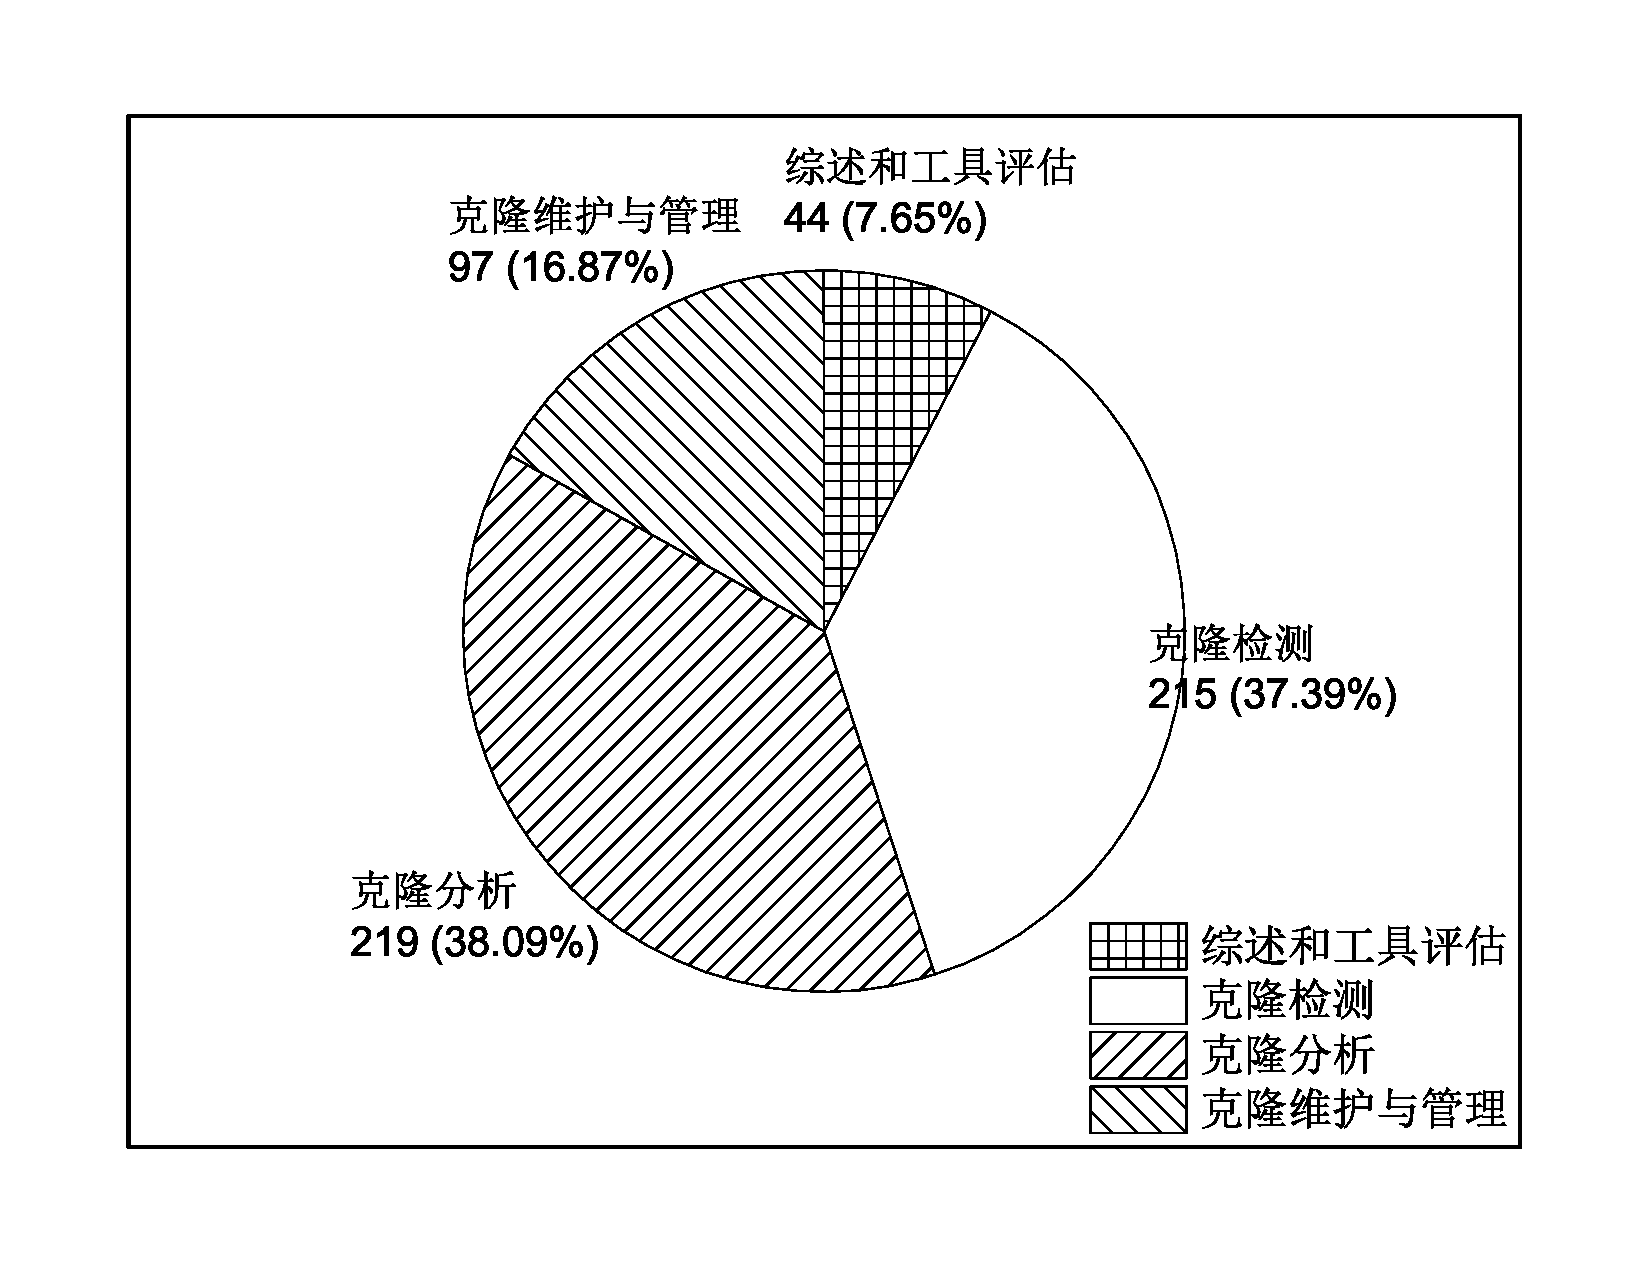
\includegraphics[width = 0.8\textwidth]{literaturedistribution1}
\bicaption[literaturedistribution1]{}{克隆代码研究领域文献分布}
{Fig.$\!$}{Literature distribution of code clone research}
%{Fig.$\!$}{Literature Distribution of Code Clone Research}
\vspace{-1em}
\end{figure}

根据此文献库中所给出的论文,Roy按照其分类进行了统计分析,分析了每个研究方向的论文分布情况和研究进展\cite{roy2014vision}。但是该文献库仅收录了2013年以前的文献,为了分析和反映克隆代码研究的最新进展、研究热点和发展趋势,本文在该文献库的基础上做了进一步的扩展,检索和收集了近几年的克隆代码相关文献,并按该文献库分类方式进行了重新统计和分析。本文统计和收集的文献共分为三类,即软件工程领域的重要国际会议论文、重要国际期刊论文以及相关学位论文。其中,重要国际会议论文为432篇,期刊论文113篇,学位论文30篇,共计575篇\footnote{本文统计的所有文献可分为两个部分:一是来源于阿拉巴马大学的文献库,二是笔者在进行研究期间所阅读整理和收集的文献。在收集的过程中,已经对文献进行了初步筛选,仅选取了领域内权威期刊、会议以及学位论文。} 。

克隆代码研究领域的文献统计分析结果如图~\ref{literaturedistribution1}~所示。从图中可以看出,目前研究中对克隆检测与分析的研究较为充分,是克隆研究领域的研究热点问题,分别占比37.39\%和38.09\%;而克隆维护与管理的研究论文占比较少(占16.87\%),说明目前对该方向的研究还方兴未艾。克隆综述和工具评估方面的研究占比更少,仅为7.65\%,说明目前较为实用的工具还不够充分。

\begin{figure}[htbp]
\centering
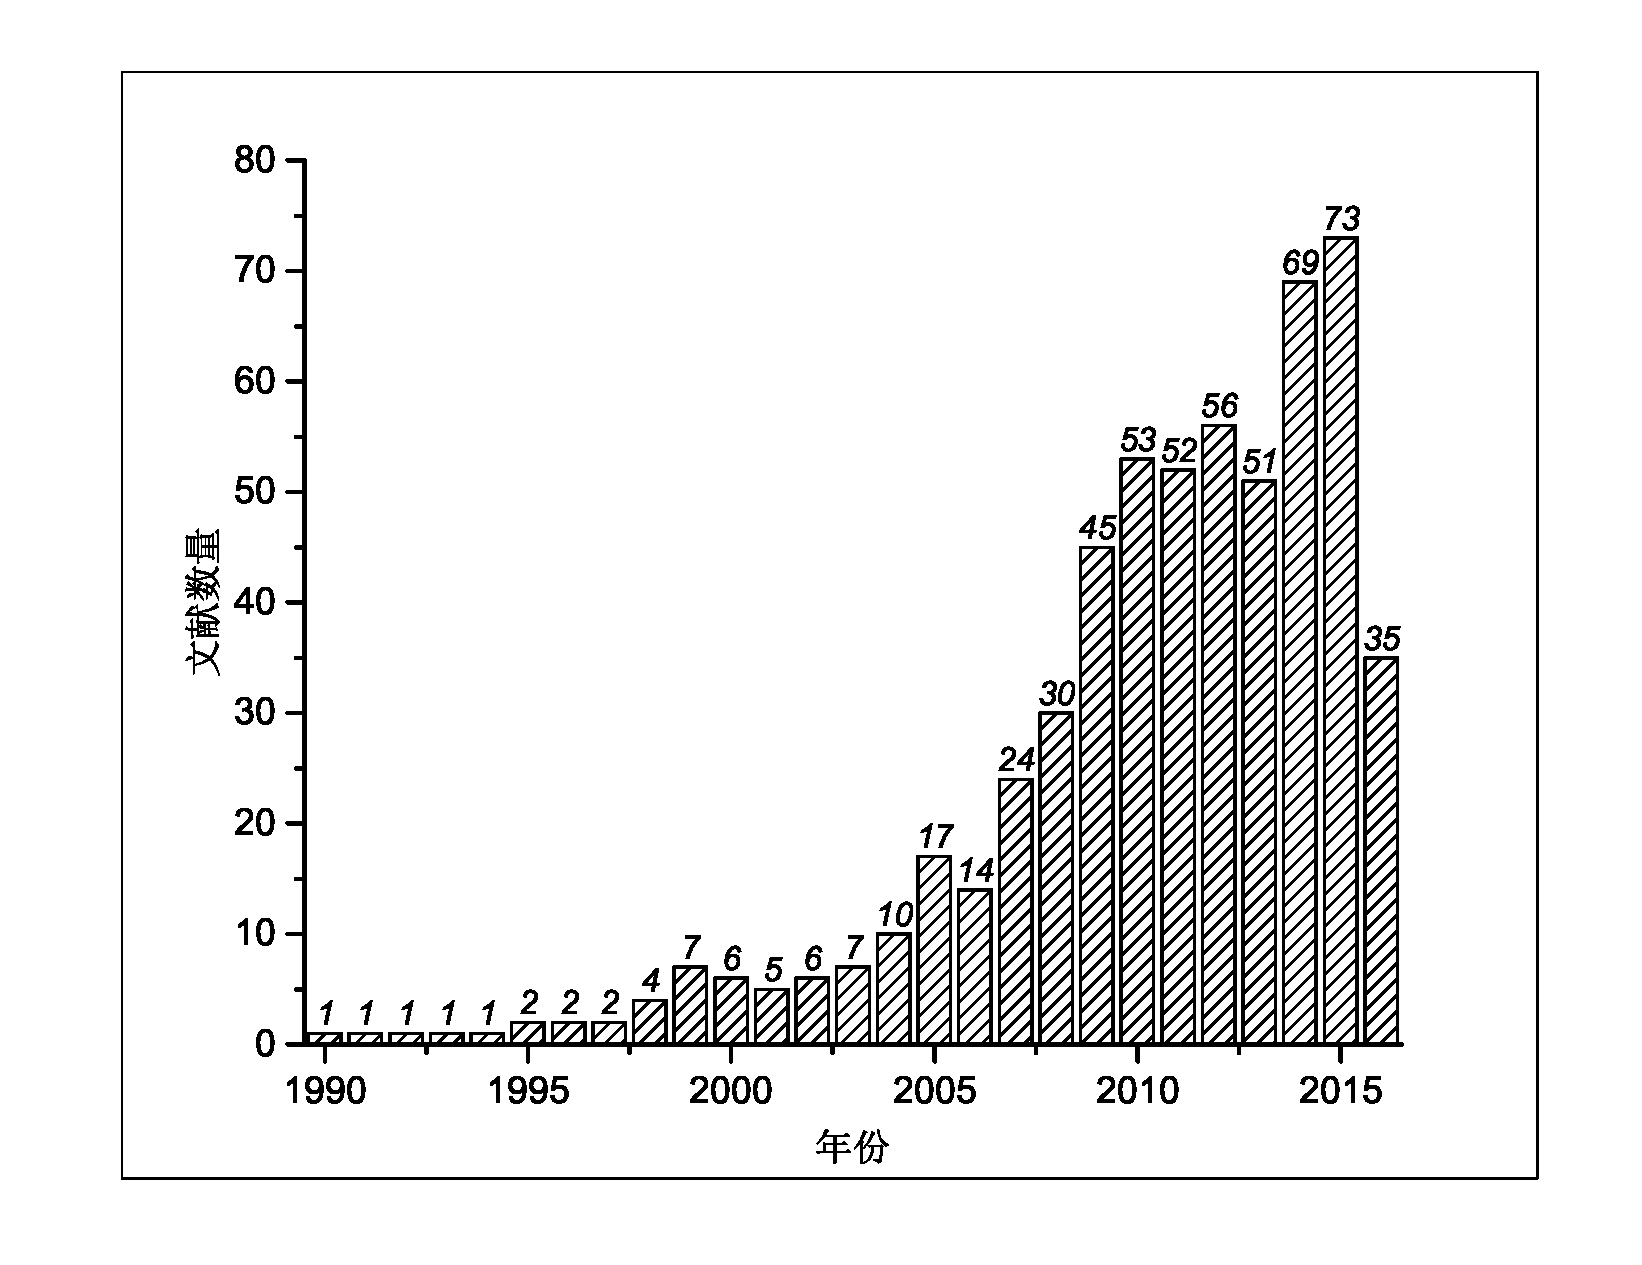
\includegraphics[width = 0.8\textwidth]{literaturedistribution2}
\bicaption[literaturedistribution2]{}{克隆领域每年发表的论文数量}
{Fig.$\!$}{Annual number of published papers of code clone research}
{Fig.$\!$}{Annual Number of Published Papers of Code Clone Research}
\vspace{-1em}
\end{figure}

\begin{figure}[htbp]
\centering
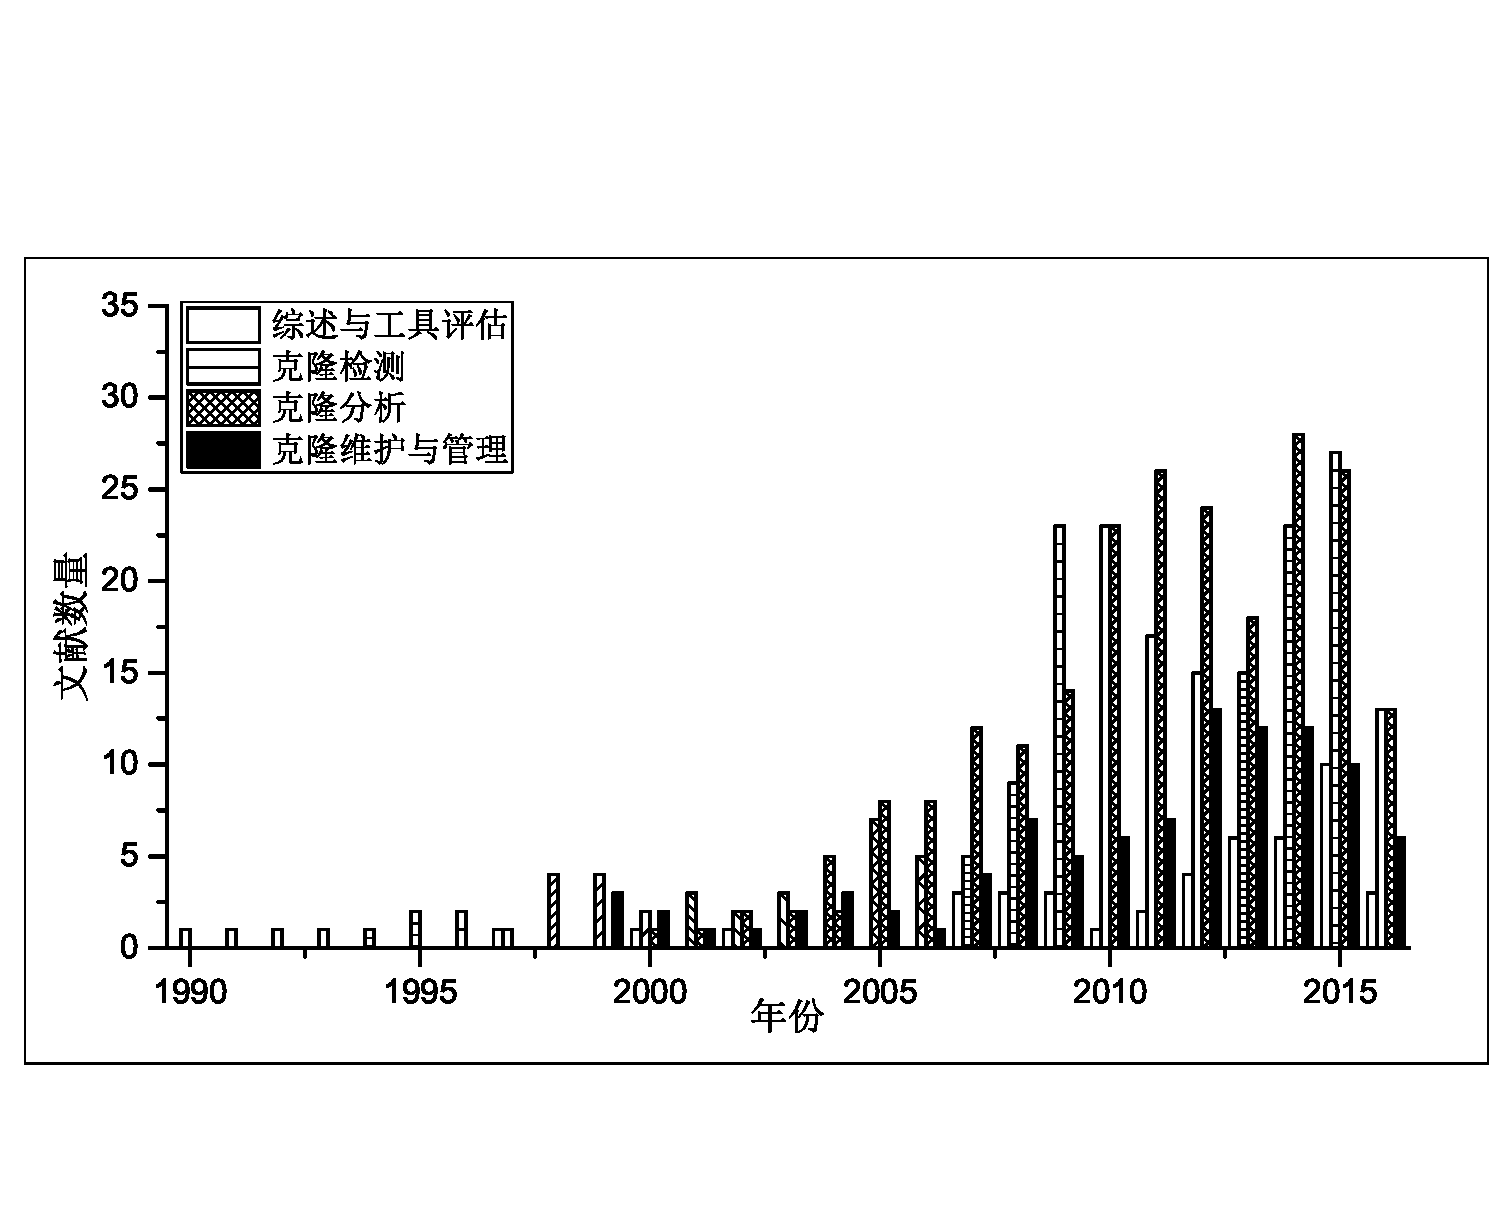
\includegraphics[width = 0.8\textwidth]{literaturedistribution3}
\bicaption[literaturedistribution3]{}{各个克隆研究活动每年发表的文献数量}
{Fig.$\!$}{Annual number of published papers of each clone research activity}
%{Fig.$\!$}{Annual Number of Published Papers of Each Clone Research Activity\vspace{-1em}
\end{figure}


为便于分析克隆代码研究领域的发展趋势,本文又对克隆代码研究领域的文献按照发表年份和研究方向进行了统计。统计分析结果如图~\ref{literaturedistribution2}~和~\ref{literaturedistribution3}~所示,其中图~\ref{literaturedistribution2}~是领域整体上每年发表文献数量的统计情况,图~\ref{literaturedistribution3}~是在不同研究方向上每年发表文献数量的统计情况。

从图~\ref{literaturedistribution2}~可以看出,克隆研究可以划分为两个阶段:1990-2003年和2004-2016年。在2003年以前,克隆代码研究领域的文献数量较少,这一阶段是克隆代码研究的孕育期。而在2004年以后的近10年内,克隆代码研究领域的文献数量快速增长,并且保持在一个较高的水平上,展现出了蓬勃的发展趋势,表明此阶段是克隆代码研究的发展期。与图~\ref{literaturedistribution2}~类似,从图~\ref{literaturedistribution3}~在不同研究方向上每年发表的文献数量来看,其研究趋势也以2003年为界限划分为两个阶段。在2003年以前,克隆代码研究主要集中在克隆检测方向,处于孕育期。在2004年以后,各个研究方向的文献数量都有了快速增长,进入了发展期。其中尤以克隆检测和分析方向的发展最为迅速,发表了大量研究成果,并依然有继续增长的趋势,说明克隆检测和分析事目前研究最为充分和最为活跃的研究方向。相比之下,克隆维护和管理仅在近几年才引起人们的关注,对克隆维护和管理的研究虽然近几年才刚开始起步,文献数量占比相对较少,但已呈现出逐年增长和后来者居上的趋势,说明克隆维护和管理正在逐渐成为克隆代码研究领域的新热点。

%\begin{figure}[htbp]
%\centering
%\subfigure{\label{literaturedistribution21}}\addtocounter{subfigure}{-2}
%\subfigure[Clone number of papers published each year in the field]{\subfigure[克隆领域每年发表的论文数量]{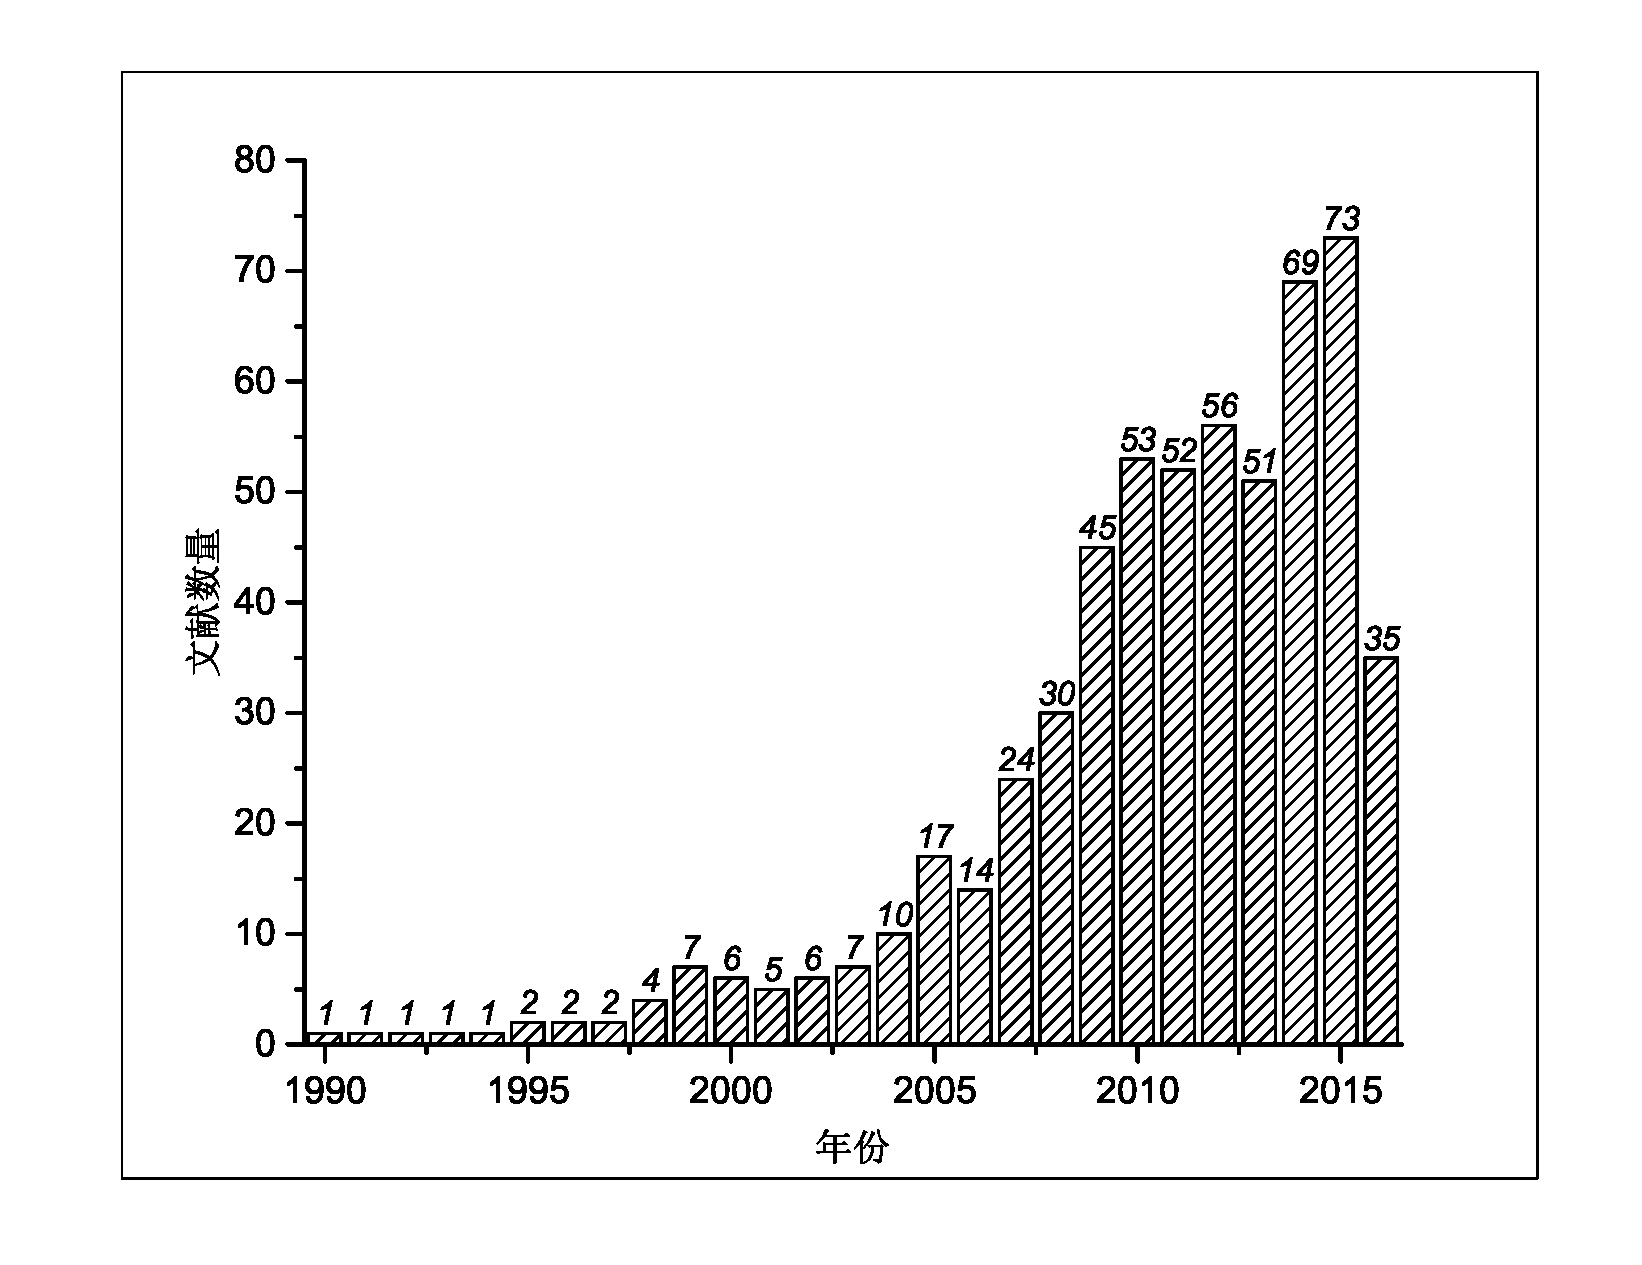
\includegraphics[width=0.8\textwidth]{literaturedistribution21}}}
%\subfigure{\label{literaturedistribution22}}\addtocounter{subfigure}{-2}
%\subfigure[Each clone number of events annually published literature]{\subfigure[各个克隆活动每年发表的文献数量]{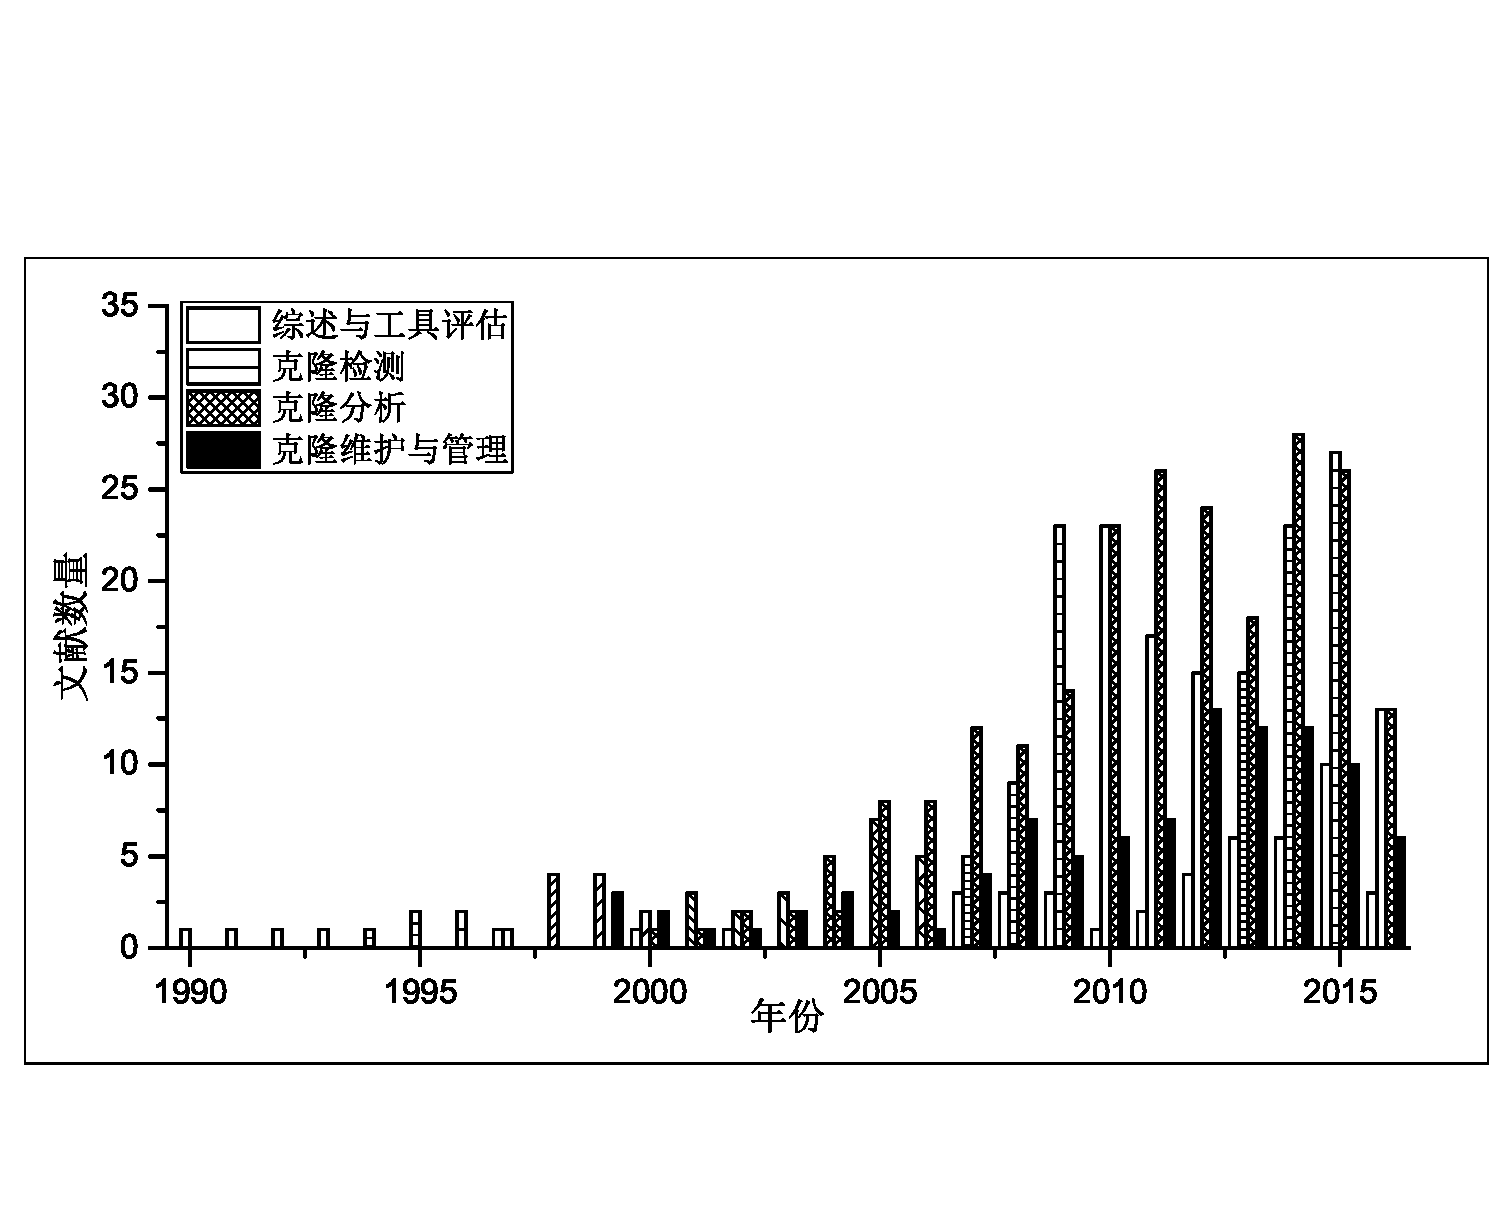
\includegraphics[width=0.8\textwidth]{literaturedistribution22}}}
%\bicaption[literaturedistribution2]{}{克隆代码领域研究趋势}{Fig.$\!$}{Cloning research trends in the code field}\vspace{-1em}
%\end{figure}

%为便于分析克隆代码研究领域的发展趋势,本文又对克隆代码研究领域的文献按照发表年份和研究方向进行了统计。统计分析结果如图~\ref{literaturedistribution2}~所示,其中图~\ref{literaturedistribution21}~是领域整体上每年发表文献数量的统计情况,图~\ref{literaturedistribution22}~是在不同研究方向上每年发表文献数量的统计情况。
%从图~\ref{literaturedistribution21}~可以看出,克隆研究可以划分为两个阶段:1990-2003年和2004-2016年。在2003年以前,克隆代码研究领域的文献数量较少,这一阶段是克隆代码研究的孕育期。而在2004年以后的近10年内,克隆代码研究领域的文献数量快速增长,并且保持在一个较高的水平上,展现出了蓬勃的发展趋势,表明此阶段是克隆代码研究的发展期。与图~\ref{literaturedistribution21}~类似,从图~\ref{literaturedistribution22}~在不同研究方向上每年发表的文献数量来看,其研究趋势也以2003年为界限划分为两个阶段。在2003年以前,克隆代码研究主要集中在克隆检测方向,处于孕育期。在2004年以后,各个研究方向的文献数量都有了快速增长,进入了发展期。其中尤以克隆检测和分析方向的发展最为迅速,发表了大量研究成果,并依然有继续增长的趋势,说明克隆检测和分析事目前研究最为充分和最为活跃的研究方向。相比之下,克隆维护和管理仅在近几年才引起人们的关注,对克隆维护和管理的研究虽然近几年才刚开始起步,文献数量占比相对较少,但已呈现出逐年增长和后来者居上的趋势,说明克隆维护和管理正在逐渐成为克隆代码研究领域的新热点。

\BiSubsection{克隆代码检测}
{Code Clone Detection }
\label{clonedetection}
克隆检测是指从软件中检测并报告克隆代码的位置的研究。相对于克隆代码研究的其他技术而言,克隆检测技术相对成熟。

\BiSubsubsection{克隆检测方法}
{Clone Detection Methods}

%%一般而言,克隆代码检测分为三个步骤:代码的中间表示、相似性匹配和报告检测结果。首先使用不同的方法对源代码进行抽象表示或转换,将其表示为抽象语法树等中间表示形式。然后对代码的中间表示形式进行相似性匹配,寻找相似的代码片段。最后报告检测结果,将彼此相似的克隆代码以克隆组的形式保存在检测结果中。
迄今为止,研究人员已提出许多种克隆检测方法,并开发了相应的检测工具。根据所使用的技术不同,可以将克隆检测划分为基于文本(Text)的方法、基于Token的方法、基于树(如Abstract Syntax Tree,AST)的方法、基于程序依赖图(Program Dependency Graph, PDG)的方法和基于度量值(Metric)的方法。

基于Text的克隆检测方法是通过直接比较源代码文本,使用字符串匹配等算法来检测克隆代码。因其并没有对源程序进行词法分析,大部分仅可以较好地支持Type 1克隆的检测。目前使用较多的基于文本的克隆检测工具主要有duploc\cite{ducasse1999language}、Simian\cite{Simian}、DuDe\cite{wettel2005archeology}、SDD\cite{lee2005sdd}、NiCad\cite{roy2008nicad}等。

基于Token的克隆检测方法是通过对源代码进行词法分析,获得源代码的Token序列,然后通过寻找Token序列中相似的子序列来检测克隆代码。因其对源代码进行了词法分析,所以可以较好地检测Type-2克隆代码的检测。但由于缺乏必要的语法和语义分析,使其无法较好地支持Type-3和Type-4克隆的检测。
目前使用较多的基于Token的克隆检测工具主要有Dup\cite{baker1995finding}、CCFinder\cite{kamiya2002ccfinder}、CP-Miner\cite{li2006cp}、iClone\cite{gode2009incremental}等。

基于Tree的克隆检测方法是将源代码表示为某种树的形式(如抽象语法树、代码解析树等),然后通过使用子树匹配算法从中寻找相似的子树来检测克隆代码。因其对源代码进行了语法分析,所以提高了克隆代码检测的准确率,尤其是可以较好地支持Type-3克隆的检测。但是由于子树匹配算法的时间复杂度高于前两种方法,因此这类算法的检测速度低于前两种方法。
目前使用较多的基于Tree的克隆检测工具有CloneDr\cite{baxter1998clone}、SimScan\cite{SimScan}、Deckard\cite{jiang2007deckard}、CloneDigger\cite{bulychev2008duplicate}等。

前三种克隆检测方法中所使用的中间表示形式较为容易实现,可使用程序静态分析方法或者编译器前端获得源代码的中间表示。大部分的克隆检测方法和检测工具属于前三种方法中的一种,可以检测系统中的大部分克隆代码。

基于PDG的克隆检测方法的主要思路是,将源代码转化成程序依赖图(包括数据依赖图和控制依赖图),然后通过寻找同构的子图来检测克隆代码。因程序依赖图表示了程序的语义信息,所以该方法可以支持语义相似的Type-4克隆代码的检测。但由于程序依赖图生成算法和图匹配算法的时间和空间复杂度极高,因而导致这类检测算法的时空开销过大,使其无法应用于大规模程序的克隆代码检测。
目前基于PDG的克隆检测工具主要有Duplix\cite{krinke2001identifying}等。

基于Metric的克隆检测方法是先将源代码转换为某种中间表示,然后在其基础上提取度量值并抽象为一个特征向量,然后通过计算特征向量的相似度来检测克隆代码。该方法的主要优点是检测速度快。但因基于度量值的方法高度依赖于度量值的提取,在对源码提取度量值的过程中会损失源码的部分语义信息,因此检测效果不够理想,使其应用受限。

此外,还有人使用结合两种或两种以上检测技术的混合方法来检测克隆代码。例如,Deckard在生成抽象语法树的基础上提取结构特征向量表示代码,然后使用聚类的方法寻找克隆代码\cite{jiang2007deckard}。CloneMiner先将源代码表示为Token形式,然后在此基础上通过使用频繁模式挖掘算法寻找相似模式来检测克隆代码\cite{basit2009data}。


\BiSubsubsection{克隆检测方法及工具评估}
{The Evaluation for Code Clone Detection Methods and Tools}

不同的克隆检测方法和检测工具各有其优缺点,分别适合检测不同类型的克隆代码,对同一类型的克隆代码的检测效果也不尽相同。如何针对具体的应用,选择合适的克隆检测方法和工具是困扰开发人员的一个问题。因此,
研究人员对主流的克隆检测方法及其检测工具进行了评估研究,以期为用户选择方法和工具提供指导性的建议\cite{bellon2007comparison}\cite{rattan2013software}\cite{roy2009comparison}\cite{svajlenko2014evaluating}。%%Bellon对6个克隆检测工具进行了评估,分别对比了查准率、查全率以及时间和空间等性能\cite{bellon2007comparison}。Rattan通过使用一种标准的系统文献综述方法,详细分析了克隆检测方面的213篇文献,并对不同的检测方法进行了评估分析,并给出了未来的研究方向\cite{rattan2013software}。此外,Roy重点分析了检测工具的使用技术和适用环境,对克隆检测工具的检测效果进行了详细的对比,对帮助用户选择和使用克隆检测工具有重要的指导意义\cite{roy2009comparison}\cite{svajlenko2014evaluating}。
本文也对目前较为主流的克隆检测工具和方法支持的克隆类型和检测效果等进行了评估,评估结果如表~\ref{detectionevaluation}~所示。其中,检测效果采用“较好”、“一般”和“较差”三种级别来评估:“较好”是指可以较好地支持该类型克隆代码;“一般”是指可以支持检测该类型克隆代码,但效果不佳;“较差”是指可以检测少部分的该类型克隆代码;对未支持的克隆类型未列出。

\begin{table}[htbp]
\bicaption[detectionevaluation]{}{主流克隆检测方法与工具评估}
{Table$\!$}{Evaluation for popular clone detection methods and tools}
\vspace{0.5em}
\centering
\wuhao
\begin{tabular}{cccc}
\toprule[1.5pt]
类型&工具或方法名&支持的克隆类型&检测效果\\
\midrule[1pt]
\multirow{5}{*}{Text} 
& Duploc\cite{ducasse1999language}&1、3&较好1,一般3\\
&Simian\cite{Simian}&1、2	&较好1,一般2\\
&DuDe\cite{wettel2005archeology}&1、3	&较好1,一般3\\
&SDD\cite{lee2005sdd}&1、3	&较好1,一般3\\
&NiCad\cite{roy2008nicad}&	1、2、3	&较好1、2、3\\
\hline
\multirow{4}{*}{Token} 
&Dup\cite{baker1995finding}&	1、2&较好1、2\\
&CCFinder\cite{kamiya2002ccfinder}&1、2&较好1、2\\
&CP-Miner\cite{li2006cp}&1、2、3&较好1、2,一般3\\
&iClone\cite{gode2009incremental}&1、2	&较好1,2\\
\hline
\multirow{4}{*}{Tree} 
&CloneDr\cite{baxter1998clone}&	1、2、3	&较好1、3,一般2\\
&SimScan\cite{SimScan}&	1、2	&较好1、2\\
&Deckard\cite{jiang2007deckard}&	1、2、3	&较好1、2,一般3\\
&CloneDigger\cite{bulychev2008duplicate}&	1、2、3	&较好1、3,一般2\\
\hline
\multirow{2}{*}{PDG} 
&Duplix\cite{krinke2001identifying}&	1、2、3、4	&较好1、2,一般3,较差4\\
&Gabel\cite{gabel2008scalable}&1、2、3、4	&较好1、2、3,一般4\\
\hline
\multirow{2}{*}{Metric} 
&Kontogiannis\cite{kontogiannis1996pattern}&	1、2、3、4	&较好1、2,较差3、4\\
&Mayrand\cite{mayrand1996experiment}&	1、2、3、4	&较好1、2,较差3、4\\
\bottomrule[1.5pt]
\end{tabular}
\end{table}

从表~\ref{clonedetection}~可以看出,基于Text的检测工具不支持Type-4克隆的检测。对Type-1克隆的检测效果最好,对Type-3克隆的检测效果一般。而对Type-2克隆支持较弱,仅有两个工具可以支持。原因是Type-2克隆是标识符重命名的克隆代码,基于Text的方法不能很好地处理标识符重命名问题。基于Token的检测工具同样不支持Type-4克隆的检测,但是可以较好地检测Type-1和Type-2克隆。支持Type-2克隆检测的原因是在将源程序转换成Token序列时进行了词法分析,因此可以解决标识符重命名的问题。但仅有一个工具可以检测Type-3克隆代码,并且检测效果一般。基于Tree的检测工具,同样不支持Type-4克隆的检测,但是对Type-1克隆的检测效果较好,并且几乎都支持Type-2和Type-3克隆的检测。由于采用的匹配算法不同,对Type-3即近似克隆的检测效果不尽相同,有些可以较好地支持Type-2克隆的检测,有些则较好地支持Type 3克隆的检测。基于PDG的检测方法不仅可以较好地检测Type-1和Type-2克隆,还可以以不同的程度支持Type-3和Type-4克隆的检测。但因其复杂度相对较高,使其并没有太多的检测工具可以利用。基于Metric的检测方法目前仅有一些检测方法被提出\cite{kontogiannis1996pattern}\cite{mayrand1996experiment},缺少相应的检测工具。

%可见,目前克隆检测方法对Type-1和Type-2克隆的检测最简单,因此效果最好,检测工具也最多;对Type-3克隆的检测相对于前两种有一定的难度,因此效果一般,但也有少量工具支持;对Type-4克隆的检测难度最大,因此效果最差,工具最少。此外,基于Text、基于Token、基于Tree的克隆检测方法实现容易,是目前较为主流的方法,相应的检测工具也较多。基于PDG的克隆检测方法受到图匹配算法复杂性的影响使得这类方法的实现难度较大,因此实用工具不多。而基于Metric的克隆检测因为检测效果不够理想,所以研究较少,也没有可用的检测工具。其次,目前绝大多数的克隆检测工具仅支持单版本的克隆代码检测,无法同时检测多个版本中的克隆代码。少数的克隆检测工具(如iClone)采用了增量式的克隆代码检测方法,即在旧版本克隆检测的基础上对新版本进行克隆代码检测,从而节约了检测时间,提高了检测效率。此外,目前绝大部分的克隆检测工具也没有集成到软件开发环境中,开发人员无法在开发过程中实时地检测和跟踪克隆代码。因此,研究如何提高Type-3和Type-4克隆的检测效果,以及如何在软件开发过程中增量式地检测克隆代码,这既是一个难点问题,也是未来的一个研究重点问题。

\BiSubsection{克隆代码分析}
{Code Clone Analysis}

克隆分析是指使用各种技术手段分析系统中的克隆代码,并挖掘其隐含的特征,旨在帮助软件开发人员更好地理解和维护克隆代码。目前的克隆分析研究主要集中在克隆演化分析、克隆评价分析上。

\BiSubsubsection{克隆代码演化}
{Code Clone Evolution}

%克隆代码往往存在于软件系统的多个版本中,并随着软件系统进行演化。
克隆代码演化分析就是通过分析克隆代码的演化过程,提取克隆代码的演化特征,识别克隆代码的演化规律,从而辅助人们更好地理解和维护克隆代码。克隆演化研究包括克隆演化过程分析和演化特征分析两个方面。演化过程分析即模型化克隆代码的演化过程。演化特征分析是分析克隆代码在演化过程中表现出来的演化特征或演化模式及其对软件质量的影响。

克隆演化过程分析最早是2001年由Antoniol等人提出的,使用时间序列描述克隆代码的演化模型\cite{antoniol2001modeling},但并未引起人们的重视。2005年,Kim提出了克隆家系模型用于描述克隆代码的演化过程,被认为是迄今为止最好的演化模型\cite{kim2005empirical}。Roy使用函数映射帮助构建克隆家系,并开发了gCad克隆家系提取器,大大提升了构建克隆家系的时间效率\cite{saha2011automatic}。Bakota通过映射不同版本的克隆来分析克隆代码的演化过程,并使用克隆坏味(Clone Smell)帮助分析克隆代码对系统的影响\cite{bakota2011tracking}。Harder对现有的演化模型进行分析\cite{harder2009modeling},指出通过分析克隆演化特征可以帮助程序开发和维护人员理解和维护克隆代码。

究竟哪些演化特征能真实准确地反映克隆代码的规律?这是克隆演化分析的难点问题。因此目前对克隆演化分析的研究主要集中在研究确定提取克隆代码的哪些特征作为演化特征以及如何提取这些特征。目前,常用的克隆演化特征主要包括克隆寿命、克隆稳定性与一致性变化。

%克隆寿命是指克隆代码在系统中的存在时间。Kim研究发现克隆代码要比非克隆代码更加稳定,同时寿命也更长\cite{kim2005empirical};进一步对长寿命的克隆代码进行研究后,发现对克隆代码的修改会使得克隆代码的寿命变短\cite{cai2011empirical}。Krinke通过对比克隆和非克隆代码,也发现克隆代码比非克隆代码的寿命更长\cite{krinke2011cloned}。通过对精确克隆和近似克隆的演化分析,发现其在演化过程中所表现出来的共同特点是:尽管克隆代码比率会随着时间而逐渐降低,但克隆代码的存在时间往往都会超过一年\cite{bazrafshan2012evolution}。因此,克隆代码会长时间的存在于系统中,在其生存期间克隆代码往往会发生变化,其变化规律与具体的软件系统相关\cite{gode2009evolution}。

%克隆稳定性关注的是在克隆代码的生存期内是否发生变化。被研究者普遍认可的观点是寿命较长的克隆代码是稳定的\cite{krinke2008cloned}\cite{gode2011clone}\cite{harder2013cloned},不会对系统造成不利的影响,也不会增加系统的维护成本。但是在克隆代码是否比非克隆代码更稳定这个问题上还存在一定的分歧。例如Gode研究发现大部分克隆是稳定的,不会发生变化\cite{gode2011frequency}。而Rahman的研究却发现克隆代码比非克隆代码更容易发生变化,是不稳定的\cite{rahman2014change}。Mondal给出了更为细致的分析结果,即Type-1、Type-2克隆是不稳定的,Type-3克隆是稳定的;并且发现克隆代码比非克隆代码的变化更分散,Type-3克隆比Type-1和Type-2克隆的变化更分散\cite{mondal2012comparative}\cite{mondal2012dispersion}。%%由此可见,在克隆代码的稳定性特征方面尚未达成共识,仍需要进一步研究。

%克隆代码的变化包括一致性变化和不一致性变化。遗忘一致性变化将会引发相关的软件缺陷,因此一致性变化也是克隆演化分析研究中需要关注的特征。Gode的研究发现发生一致性变化的克隆代码占克隆代码的比例很小\cite{gode2011frequency}。Krinke的研究进一步发现发生一致性变化和不一致性变化的克隆代码比例大约各占一半,并且大部分发生不一致性变化的克隆代码在后续的演化过程中不会继续发生变化\cite{krinke2007study}。Mondal等人的研究发现发生一致性变化的克隆代码可能会导致延迟传播现象。延迟传播是指某一个克隆片段的变化没有立即传播到其所在的克隆组中,而在间隔一定数量的版本后传播,继续发生一致性变化。研究表明延迟传播在Type-3的克隆中出现的更为频繁,软件开发人员应该重点关注Type-3克隆代码的变化,以避免引入克隆代码相关的软件缺陷\cite{mondal2016comparative}。

表~\ref{characteristic}~列出了目前对克隆演化特征的研究情况。由表中可以看出,研究者较为关注的克隆演化特征是克隆寿命、克隆稳定性与一致性变化。上述三个特征并不是相互独立的,克隆寿命会受到稳定性和克隆变化的影响,同时克隆稳定性与克隆变化之间存在对立关系。对克隆演化分析的研究大多属于实证研究,往往会较多地依赖于具体被用于实验分析的软件系统,这就导致了不同的研究可能得出不同的结论。例如对克隆稳定性的研究就出现了截然相反的观点。尽管如此,克隆演化特征分析依然可以给开发人员提供有价值的建议。一个普遍的共识是在维护和管理克隆代码的过程中更应关注那些克隆寿命较短、稳定性较差、发生一致性变化的克隆代码。%%但克隆寿命、克隆稳定性和一致性变化之间究竟存在着怎样的关系,它们对软件质量究竟会产生怎样的影响,还有哪些影响软件质量的克隆代码特征,还有待进一步深入的研究。

\begin{table}[htbp]
\centering
\bicaption[characteristic]{}{克隆演化特征分析}
{Table$\!$}{The analysis of clone evolutionary characteristic}
\vspace{0.5em}
\wuhao
\begin{tabularx}{0.9\textwidth}{llX}
\toprule[1.5pt]
文献&克隆模式、特征&结论\\
\midrule[1pt]
\cite{kim2005empirical}&	克隆寿命/一致性变化	&观察并分析克隆家系寿命与一致性变化规律\\
\cite{cai2011empirical}&	克隆寿命&	克隆寿命与克隆修改次数、新增和减少有关\\
\cite{krinke2011cloned}&	克隆寿命&	克隆代码的寿命比非克隆的寿命更长\\
\cite{bazrafshan2012evolution}\cite{gode2009evolution}&	克隆比率/寿命/变化规律	&克隆比率会随时间降低,会存在超过一年,存在期间变化规律往往和具体系统相关\\
\hline
\cite{krinke2008cloned}&克隆稳定性&	克隆代码比非克隆代码更稳定\\
\cite{gode2011clone}\cite{harder2013cloned}&	克隆稳定性&	克隆代码十分的稳定\\
\cite{gode2011frequency}&	克隆变化/一致性变化&	大部分克隆不会变化,一致性变化会更少\\
\cite{rahman2014change}&	克隆稳定性&	克隆会比非克隆更容易发生变化\\
\cite{mondal2012comparative}\cite{mondal2012dispersion}&	克隆稳定性/变化分布&	Type-1、Type-2是不稳定的,Type-3是稳定的;发现克隆代码变化比非克隆更加分散,同时Type-3克隆比Type-1和Type-2更加分散\\
\hline
\cite{krinke2007study}&	一致性变化&	一半的变化是不一致变化,且发生不一致性变化后,在后续的时间内会保持这种变化\\
\cite{mondal2016comparative}&	延后传播&	Type-3更容易发生延后传播并导致缺陷\\
\bottomrule[1.5pt]
\end{tabularx}
\end{table}


\BiSubsubsection{克隆代码评价}
{Code Clone Evaluation}

克隆评价分析主要是分析克隆代码对系统产生的影响,以便辅助开发人员更好地理解和维护克隆代码。克隆代码是否有害一直是克隆评价关注的一个热点,也是争论的一个焦点问题。因此,克隆评价研究主要是围绕着克隆代码是否有害而展开的,只是在不同阶段,人们对克隆代码的态度有所不同,研究的关注点也因此有所不同而已。

在研究的初始阶段,人们大多倾向于认为克隆代码都是有害的,因而研究的侧重点是克隆代码是否会引发软件缺陷(即克隆代码相关的缺陷分析),以及克隆代码是否会增大系统的维护代价(即克隆代码的维护代价分析)。然而随着对克隆代码研究的深入,人们研究发现虽然克隆代码有时会对软件质量产生一些负面影响,但并不一定都是有害的,从而引发了对克隆代码有害性的讨论(即克隆代码的有害性分析)。因此,克隆评价主要包括克隆相关的缺陷分析、克隆维护代价分析、克隆有害性分析等。

%在早期,有人认为克隆代码是一种最刺鼻的代码坏味,是因为它有可能会引发相关缺陷。因此,人们研究的关注点主要集中在克隆代码的缺陷分析上。例如,Juergens等人研究发现克隆代码的不一致性变化会引发相应的软件缺陷,从而降低了软件质量\cite{juergens2009code}。Gauthier通过对克隆代码进行安全性分析,在开源软件Joomla和Moodle中发现了几个潜在的影响软件质量的安全漏洞和缺陷\cite{gauthier2013uncovering}。但也有另外一些证据表明克隆代码的不一致性变化并不一定会引发缺陷,因此不会对软件质量产生显著的影响。例如,Bettenburg对不一致性变化是否引发缺陷的研究发现,仅有极少数的不一致性变化会引发缺陷\cite{bettenburg2009empirical}。文献\cite{wagner2016relationship}的研究则表明Type 3克隆代码中大约有17\%的代码含有缺陷,并且Type 3克隆不容易发生不一致性变化。文献\cite{elish2015fault}通过对缺陷密度的分析发现,面向对象程序中的克隆类含有更少的缺陷,并且Type 3克隆含有的缺陷最少。因此有人将克隆代码研究应用到缺陷检测中,但没有直接证据证明克隆代码与缺陷密切相关\cite{lo2012active}\cite{kamei2011empirical}。%%因此,克隆缺陷分析并不能直接证明克隆代码是有害的。

%除了克隆相关的缺陷分析外,还可以从维护代价的角度去分析克隆代码对软件产生的影响。Harder通过实验发现克隆代码的存在并不会增加缺陷修复的时间,但是缺陷未被修复则可能导致维护代价的增加\cite{harder2012controlled}。Lozano通过研究克隆代码的可变性,也发现克隆代码的存在会增加软件维护的代价\cite{lozano2008assessing}。Juergens不仅认为克隆代码会增加维护代价,还提出了一个计算模型来计算克隆维护代价\cite{juergens2010much}。而Monden的研究则发现包含少量克隆代码的软件模块比不含克隆代码的软件模块更可靠,但含有大量克隆代码的软件模块则正相反,实验表明克隆代码与软件可靠性和维护代价有一定的关联,但这种关联关系并不十分明确\cite{monden2002software}。以上维护代价分析的研究表明克隆代码的存在有可能会增加软件的维护代价,但是如何定量地计算克隆代码引起的维护代价仍然是一个尚未解决的问题。

%%虽然缺陷分析和维护代价分析可用于评价克隆代码对软件产生的影响,但却不能作为评价克隆代码是否有害的直观证据。正因如此,近些年来,研究人员又展开了克隆代码有害性分析的研究。Kapser通过对比11种克隆模式在软件开发和维护过程中的优缺点,并在开源软件Apache和Gnumeric上进行实证研究,发现在Apache中大约有71\%的克隆代码被分类为有益克隆,对系统维护具有积极的影响,是一种合理的存在方式,因此人们应当正视在开发过程中克隆代码的长期存在\cite{kapser2006cloning}\cite{kapser2008cloning}。Kapser通过对Apache Web Server中的克隆代码进行分析,研究发现其中一个子系统中聚集了大量的克隆代码;该子系统的克隆代码增加了系统的功能性,对软件开发过程是有益的\cite{kapser2006supporting}。Selim使用风险模型判定克隆代码是否有害,研究结果发现克隆代码并不比非克隆代码具有更高的有害风险\cite{selim2010studying}。Wang提出利用贝叶斯网络对克隆代码进行有害性预测的方法\cite{wang2012can},该方法可用于辅助开发人员决定是否可以通过复制粘贴的方式引入新的克隆代码。Higo则提出一种提取有问题的克隆代码(有害克隆)的方法,该方法先对程序进行标准化,然后利用检测工具检测克隆代码,最后对检测到的克隆代码进行过滤、合并等操作来提取有问题的克隆代码,在Linux内核2.6.6上的实验结果表明只有少数克隆代码是有问题的克隆代码\cite{higo2009problematic}。Hordijk提出了一个结构化的证据模型分析克隆代码的有害性,研究结果表明只有少部分的证据证明克隆代码是有害的,并且仍需更多的研究去支撑这一结论\cite{hordijk2009harmfulness}。%%从上述对克隆代码有害性分析的结果不难得出结论,克隆代码并非都是有害的,但是究竟具有什么特征的克隆代码是有害的,还是一个有待深入研究的问题。

表~\ref{evaluation}~对克隆评价分析研究进行了分类统计,使用“积极”、“中立”和“消极”三种评价标准对现有的克隆评价分析方法进行了总结。“积极”是指克隆代码的存在对系统有积极的影响;“中立”是指克隆代码不会对系统产生影响;“消极”是指克隆代码会对系统产生消极的影响。从表中可以看出,大部分研究对克隆代码持积极和中立的态度,仅有少数持消极态度。这从另外一个侧面表明目前对克隆代码是否有害还存在一定的分歧,主要原因是对克隆代码缺少统一的评价标准以及深入的特征挖掘与分析。%%,当然这也是克隆评价分析中的最具挑战性的问题。

\begin{table}[htbp]
\centering
\bicaption[evaluation]{}{克隆评价分析}{Table$\!$}{The analysis of clone evaluation}\vspace{0.5em}\wuhao
\begin{tabularx}{0.9\textwidth}{lllX}
\toprule[1.5pt]
&文献&评价&结论\\
\midrule[1pt]
\multirow{6}{*}{\rotatebox{270}{克隆缺陷分析}} 
&\cite{juergens2009code}&消极&研究发现不一致变化在克隆中发生较为频繁,同时也会导致相应的缺陷\\
&\cite{gauthier2013uncovering}&消极&通过对不安全的克隆代码分析,发现了几个安全漏洞和缺陷\\
&\cite{bettenburg2009empirical}&积极&克隆代码的不一致变化并不会引入缺陷,不会对软件的质量产生影响\\
&\cite{elish2015fault}&积极&克隆代码含有更少的缺陷,Type 3所含有的缺陷最少\\
&\cite{lo2012active}&中立&克隆代码研究应用到缺陷检测中,但没有直接证据证明与缺陷相关\\
&\cite{kamei2011empirical}&中立	&通过实验发现并不会增加缺陷修复时间,但是缺陷未被修复,可能会产生维护代价的增加\\
\midrule[1pt]
\multirow{4}{*}{\rotatebox{270}{克隆维护代价分析}} 
&\cite{wagner2016relationship}&中立	&Type 3克隆中有17\%含有缺陷,并且Type3克隆更容易发生一致性变化\\
&\cite{harder2012controlled}&消极&通过对克隆代码的可变性研究发现克隆代码确实会增加其方法可变化的维护代价,但没有确切的证明会说明克隆会增加系统维护代价\\
&\cite{juergens2010much}&消极&认为克隆会增加维护代价,并且提出了一个代价计算模型计算这次代价\\
&\cite{monden2002software}&中立&Monden却发现包含克隆的模块比不含克隆的模块更可靠,同时含有大量克隆的模块却相反实验表明了克隆与系统可靠性和维护代价的关系,但是这种关系仍然不够明朗\\
\midrule[1pt]
\multirow{6}{*}{\rotatebox{270}{克隆有害性分析}} 
&\cite{selim2010studying}&积极&克隆代码并不比非克隆代码具有更高的有害风险\\
&\cite{kapser2006cloning}\cite{kapser2008cloning}&积极	&发现最多有71\%的克隆对系统的可维护性具有积极的影响\\
&\cite{rahman2012clones}&积极	&克隆并不是真正的代码坏味,克隆是无害的\\
&\cite{wang2012can}&中立	&预测克隆有害性,其中有害的较少,无害的较多\\
&\cite{higo2009problematic}&中立&使用分类模型抽取有问题的克隆代码,只有少部分是有问题的克隆\\
&\cite{hordijk2009harmfulness}&中立&现有研究不能支撑克隆有害的观点,仍需进一步的研究\\
\bottomrule[1.5pt]
\end{tabularx}
\end{table}

\BiSubsection{克隆代码维护}
{Code Clone Maintenance}

克隆维护是解决克隆代码问题的直接途径,主动地解决克隆代码可能或已经引发的问题。克隆维护与软件开发过程结合得较为紧密,维护的方法主要包括克隆重构、克隆规避、克隆复用和克隆管理。

\BiSubsubsection{克隆代码重构}
{Code Clone Refactoring}

重构作为一种常见的软件维护手段,是指在不改变软件外部行为的条件下改变软件的既有设计\cite{kerievsky2006重构与模式}。重构应用于克隆维护中,指的是通过重构手段消除系统中的克隆代码。

由于重构所需的条件较为苛刻,同时重构的代价也较大,还需考虑重构安全的问题。因此,在重构前对克隆代码进行可重构性分析和重构排序显得尤为重要。可重构性分析旨在识别适于重构的克隆代码候选集合,以提高克隆重构的效率。Lin等人通过对克隆代码进行差异性分析,帮助开发人员决定是否进行重构操作和如何执行重构操作\cite{lin2014detecting}。Mende实现了一个工具支持可重构性分析,在软件中识别可以被重构的函数克隆\cite{mende2009evaluation};Schulze提出了一个用于识别可重构的克隆代码的克隆分类方法,通过计算克隆代码的可重构指数识别可重构的克隆代码\cite{schulze2008towards};Choi等人提出了基于度量值的可重构性分析方法,可以快速地识别可重构的克隆代码\cite{choi2011extracting}。识别可重构克隆后,为了节省重构时间,还可以对克隆代码进行重构排序或者调度。如Mandal先通过分析克隆演化模式来确定克隆候选,然后使用关联规则挖掘进行可重构排序、\cite{mandal2014automatic};Lee采用遗传算法对重构进行调度,以确定重构顺序帮助改进软件质量\cite{lee2011automated};Zibran提出一种极限编程方法对克隆代码进行重构调度\cite{zibran2011constraint}。另外,Liu等人提出了一个重构调度方法帮助优化调度过程\cite{liu2012schedule}。尽管该方法不是针对克隆重构的,但也可以考虑将其应用于克隆代码的重构调度上。此外,Radhika等人仅考虑重构代价对所有的克隆代码进行重构排序,未考虑克隆代码是否适合重构的问题\cite{venkatasubramanyam2013prioritizing},应该结合可重构性分析指导克隆重构。
克隆重构最主要的目的是消除系统中的克隆代码。Higo等人开发了一个工具ARIES,根据克隆代码的结构信息识别可重构的克隆代码,然后通过计算不同的度量值来确定使用哪一种目前已有的重构方法移除克隆代码\cite{higo2008metric}。Krishnan通过分析克隆代码的程序依赖图,确定给定克隆代码能否被安全的重构,然后通过检测和参数化克隆代码的差异点对克隆代码进行重构,取得了较好的效果\cite{krishnan2014unification}。Barbosa使用四种规则重构克隆代码,并在开源软件JhotDraw上进行了实验,结果表明基于规则的重构方法可以有效地移除软件中的克隆代码\cite{barbosa2013removing}。

在重构完成后,对重构后代码进行分析,还可以得出一些结论以进一步指导克隆重构。G{\"o}de通过对维护人员使用的重构方法和被重构的克隆代码进行实证研究,发现在不同的软件系统中都存在克隆重构的行为,并且克隆重构不是经常性地发生而是有选择性地发生\cite{gode2010clone}。Zibran等人通过克隆重构研究,回答了所提出的关于克隆重构的七个研究问题,并且研究发现克隆规模对克隆重构没有重要的影响,同时在软件早期的版本中重构会较为频繁地发生,发生重构的克隆在重构前往往是较为稳定的克隆代码\cite{zibran2013evaluating}。Choi通过对重构行为进行观测,识别出几种较为频繁的克隆重构模式,并且分析了每种重构模式的特征,这些都有助于进一步指导克隆代码的重构\cite{eunjong2014investigation}。Tairas通过对克隆代码的重构性分析,提出了子克隆的概念,并研究发现子克隆的重构行为更容易发生,因此建议在对克隆代码的维护过程中应重点考虑子克隆的重构\cite{tairas2010sub}。

%%目前,虽然已有重构方法以插件的形式集成到了eclipse中 ,支持在软件开发过程对一般代码坏味重构。由于一般代码坏味的重构方法不一定适合克隆代重构,所以尚未有在软件开发环境中针对克隆代码的重构方法。此外,重构是在克隆代码出现后用以消除克隆代码的一种被动的软件维护方法,而且并非所有的克隆代码都适合重构。因此重构不是解决克隆代码维护难题的最有效的方法,更有效的方法是在软件开发过程中主动地规避或维护克隆代码,这是克隆维护中的一个难点问题。

\BiSubsubsection{克隆代码规避}
{Code Clone Prevention}

克隆规避也称克隆预防,是在克隆产生时通过某种策略或手段进行干预,以避免克隆代码的产生。克隆规避是一种预防性的克隆维护方法,通过阻止克隆代码产生来降低克隆维护的代价。

软件开发人员的复制粘贴活动是导致克隆代码产生的最主要原因。因此在复制粘贴时对新产生的克隆代码进行分析,帮助软件开发人员决定是否规避克隆代码,是目前常见的克隆规避方法。Ali曾提出一个克隆规避的概念模型\cite{ali2013enhancing},尽管对克隆规避研究具有一定的指导意义,但并未给出该模型的具体实现方法。Wang等人基于贝叶斯网络在复制粘贴时预测克隆代码的一致性变化,通过判断一致性变化决定是否规避该新产生的克隆代码\cite{wang2012can}\cite{wang2014predicting}。Ravikanth通过分析复制粘贴操作的前置和后置条件,来确定是否允许对被复制的克隆代码实施粘贴操作,从而实现克隆规避\cite{venkatasubramanyam2012method}。

%%由于受软件复用的影响和编程语言的限制,大部分克隆代码是无法避免的。克隆规避可以作为一种辅助的手段通过限制开发人员在软件开发过程中的复制粘贴操作帮助减少克隆代码的产生,但却无法规避全部的克隆代码。在实际的应用中,还需要将克隆规避和克隆管理相结合,对可以规避的克隆代码采用规避技术进行主动地规避,对无法规避或者无需规避的克隆代码采用跟踪的方式进行管理,以主动地维护这些代码。

\BiSubsubsection{克隆代码复用}
{Code Clone Reuse}

在软件开发过程中,复用既有代码是一种常见的软件开发手段。近些年来,随着对克隆代码评价分析研究的深入,人们已经意识到复用健壮性好的克隆代码不仅有助于缩短软件开发周期,还有利于提高软件的健壮性和可维护性。%%因此,对克隆复用的研究在近些年来引起了人们的关注,成为克隆代码领域中的一个新的研究方向。不过,相对于克隆检测和分析而言,目前对克隆复用的研究还相对较少。

Krutz等人提出克隆数据库概念,将已有克隆代码组织为克隆数据库,并结合代码检索技术实现对克隆代码的复用\cite{krutz2014code}。Ishihara提出的方法也允许开发人员通过代码搜索技术搜索可以复用的克隆代码\cite{ishihara2013reusing}。Ohta通过对比软件开发过程中由复制粘贴操作产生的克隆代码和系统中已存在的克隆代码,并将该克隆代码划分为较差、较好、最好三种情况,辅助开发人员决定是否能够复用该克隆代码\cite{ohta2015source}。但该方法对克隆代码的可复用性评价仅依赖于开发人员的复制粘贴操作,仅在复制粘贴操作发生后给出可复用性建议,无法在复制粘贴操作发生前为开发人员提供可复用的克隆代码信息。在软件开发过程中直接向开发人员提供一个已经通过某种评价方式确定是否可复用的克隆代码库,是一种更为主动的克隆代码复用形式。例如,Yang\cite{yang2015classification}等人使用机器学习模型对克隆代码进行分类,分类标准由开发人员动态地标记,通过标记可复用的克隆代码将该方法应用于克隆复用,辅助开发人员搜索可以复用的克隆代码。Ohtani从代码建议的视角辅助开发人员复用已有的代码,从不同粒度(关键字级别、方法级别和混合方法)对可复用的代码提供搜索支持,实验结果表明混合方法可以更精确地提供代码是否可复用的建议\cite{ohtani2015level}。Kintab实现了一个克隆代码的专家推荐系统,可以在线向软件开发人员提供复用克隆代码的相关咨询,软件开发人员可以根据专家的建议决定如何复用和维护既有的克隆代码\cite{kintab2014recommending}。

%%软件复用在提高软件开发效率的同时,势必也导致产生大量的克隆代码,这就使得克隆复用研究面临着一些新的问题。例如,如何实时地跟踪、维护和管理一个可复用的克隆代码库,在保证软件开发质量的前提下,主动地复用既有代码,以提高软件开发效率,既是一个新问题,也是一个难点问题。

现有的克隆代码复用研究大都是针对单一项目的。如何实现对跨项目的克隆代码复用是克隆复用面临的另一个新问题。目前,在互联网环境下,大量的开源社区里也普遍存在代码复用的情况,由此产生了跨项目的克隆代码和对跨项目代码复用的应用需求。但目前对这种跨项目的克隆代码复用的研究依然较少。Ishihara对跨项目的软件进行函数克隆检测,试图建立一个公用函数库用于代码复用\cite{ishihara2012inter}。Cheng等人研究了跨项目的克隆代码检测技术\cite{cheng2016feasibility}。Tairas等人将信息检索技术与克隆代码分析相结合,以便快速有效地搜索可复用的克隆代码\cite{tairas2009information}。事实上,以上这些技术都可以用于跨项目的克隆代码搜索和复用中。

\BiSubsubsection{克隆代码管理}
{Code Clone Management}

%%克隆代码的重构是在克隆代码产生之后消除克隆代码及其对系统产生的影响,这种维护方式属于一种较为被动的维护方式,其维护代价本来就较高。而克隆代码往往又会随时间的推移和需求的变更而在软件系统中发生变化或者产生新的克隆代码,频繁地重构势必进一步增大克隆代码维护的代价。如果将克隆代码的维护提前到软件开发阶段,在软件开发过程中跟踪克隆代码的变化,并主动地规避克隆代码的产生,则势必会降低后期维护的代价。而若要实现这种主动的维护方式,则需要从克隆代码管理的角度解决克隆代码的维护难题,即通过在软件开发过程中实现边开发、边管理克隆代码,以主动的方式维护克隆代码,消除克隆代码对软件系统的不利影响。

克隆代码管理(简称克隆管理)的概念最早是1997年由Koschke提出的\cite{koschke2008frontiers},但当时并未引起人们的重视。随着克隆代码规模的逐渐增大,人们发现现有手段无法有效解决克隆代码维护难的问题时,才开始把目光重新转向对克隆管理的研究。目前克隆管理被认为是解决克隆代码维护难题的最有效的方式。早在2012年的面向工业界的克隆管理会议\footnote{Software Clone Management Towards Industrial Application}中,就有专家学者指出克隆管理是未来的重要研究方向,如何将克隆管理与软件开发过程相结合并使之适用于工业界是目前克隆研究领域急需解决的问题\cite{koschke2012software}。%%但是目前人们对克隆管理的研究仍处于起步和理论研究阶段,罕有从管理的角度维护克隆代码的研究报道。

%Koschke将克隆管理划分为预防性、补偿性和改正性三种类型\cite{koschke2008frontiers}。预防性克隆管理的目标是避免克隆代码,关注于避免新的克隆代码的产生,而不是对已有克隆代码的管理。补偿性克隆管理的目标是发现克隆代码所引发的问题,并对其对系统造成的不利影响进行补偿。改正性克隆管理的目标是以主动的方式消除可能对系统产生不利影响的克隆代码。然而,Koschke对克隆管理的这种划分方法的理论意义大于实际意义。目前克隆管理研究主要集中于补偿性克隆管理,而改正性克隆管理尚未具体应用到实际的克隆管理中。

%Roy在文献\cite{roy2014vision}中对克隆管理研究进行了详尽的阐述,指出目前对克隆管理的研究依然较少,尚缺少有效的克隆管理方法,尤其是对Type 3和Type 4克隆代码进行管理的研究还不够充分,未来应针对这两种类型的克隆代码的管理进行深入研究。尽管Roy对克隆管理的分析涵盖了克隆代码领域的大多数研究内容,但只是以工作流的形式组织这些研究内容,并未考虑这些研究内容之间的联系,彼此之间的信息是相互割裂的,同时也没有结合软件开发过程分析对克隆管理的要求,更没有给出具体的克隆管理方法。

克隆代码管理的主要目的是降低克隆代码维护的代价。目前克隆管理的研究内容主要包括克隆跟踪、克隆变化管理以及克隆管理工具。其中,克隆跟踪是研究跟踪克隆代码产生和变化的方法。克隆变化管理是研究对克隆代码的变化进行管理的方法。克隆管理工具是研究开发有效管理克隆代码的工具。

克隆管理需要解决的首要问题是如何实时地跟踪系统中的克隆代码,包括克隆代码的产生及其变化。由于复制粘贴操作是导致克隆产生的主要原因,因此对克隆跟踪的研究主要是通过监测程序员的复制粘贴操作来实现的。例如,许多克隆跟踪工具CLONEBOARD\cite{de2009managing}、CnP\cite{hou2009cnp}、CPC\cite{weckerle2008cpc}、CReN\cite{jablonski2007cren}、CSeR\cite{jacob2010actively}等都是在软件集成开发环境中跟踪克隆代码的产生,但并非都能跟踪克隆代码的变化。另一方面,在软件开发过程中克隆代码可能随时发生变化,因此要实现对克隆代码的管理,不仅要跟踪克隆代码的产生,还要跟踪克隆代码的变化。Duala使用克隆区域描述符描述生成克隆代码的上下文信息,然后根据这些上下文信息实时跟踪克隆代码的变化\cite{duala2008clonetracker}\cite{duala2010clone}。该方法仅通过实验验证可以跟踪克隆代码的变化,但是并没有实现可用的插件集成到集成开发环境中,以实现对克隆代码的边开发、边管理。

跟踪克隆代码的目的是为了对克隆代码进行维护和管理。为了实现边开发、边管理克隆代码,还要对克隆代码的变化进行维护和管理。Yamanaka等人\cite{yamanaka2013applying}将克隆变化与事件通知机制相结合,将每一个克隆变化都看成一个事件,在克隆发生变化时提醒开发人员及时地对克隆变化进行维护。Cheng等人\cite{cheng2016rule}提出了一个基于Token的克隆代码一致性维护方法,当克隆组内的一个代码发生变化时,能够同时修改组内的其他克隆代码,保证克隆代码的一致性。该方法的前提是已知克隆变化需要一致性维护,但没有给出克隆变化是否需要一致性维护的判定方法。因此,Zhang等人\cite{zhang2016predicting}在克隆代码发生变化时预测克隆代码一致性维护需求。该方法通过提取克隆代码的演化信息及其相关特征,在克隆代码发生变化时辅助开发人员确定克隆变化是否需要一致性维护。Mondal等人通过对克隆组内的克隆代码排序,从而预测需要一致性维护的克隆代码\cite{mondal2014prediction}。此外,Murakami等人在克隆代码未发生变化时,预测克隆代码的下一次变化\cite{murakami2014predicting}。该方法通过分析历史版本中的克隆代码的变化情况,提取相关的特征进行变化预测,以便在软件开发过程中提醒开发人员对有可能发生变化的克隆代码进行维护。可见,克隆变化管理的关键不仅需要实时跟踪克隆代码的变化,更重要的是对发生变化的克隆代码进行及时的维护。

前面的研究只是针对不同的侧重点提出的克隆管理方法,却没有提供可以实际应用的克隆管理工具。鉴于此,Zhang基于事件通知机制实现了一个克隆管理工具,不仅可以监测克隆代码的产生,还可以监测克隆代码的维护过程\cite{zhang2013towards}。Nguyen实现了一种可用于管理克隆代码的eclipse插件JSync\cite{nguyen2012clone}。该插件支持在软件开发过程中对克隆代码进行克隆关系管理与一致性维护管理。这里的克隆关系管理是指在软件开发过程中检测系统中的克隆代码,并对具有克隆关系的代码进行管理。这里的一致性维护管理是指识别变化的克隆代码以及变化的克隆代码是否会导致不一致性缺陷,以便开发人员对克隆代码进行一致性维护。而另一个较早提出的eclipse插件CeDAR\cite{tairas2012increasing}。虽然没有强调是一种克隆管理工具,但事实上也具有一定的克隆管理功能。该插件将克隆检测和克隆重构融为一体,对现有克隆检测工具的克隆检测结果进行可重构性分析,寻找潜在的可重构的克隆代码,然后在软件开发过程中实现对克隆代码的重构。

%%如何将克隆代码的检测、分析和维护结合到软件开发过程中,以实现对克隆代码的边开发、边维护和边管理是克隆管理急需解决的一个难点问题。

\BiSubsection{当前研究中存在的问题分析}
{Problems in Current Research}

克隆代码研究已经成为了软件工程领域的一个热点问题,目前的克隆研究已经取得了相当丰富的研究成果,如克隆检测、克隆分析和克隆维护研究等,但目前的研究中仍然存在一些问题。

(1)克隆检测研究可以帮助程序开发人员快速的获得系统中的克隆代码,是目前研究的较为深入且广泛的一个研究活动。已经开发和提出了相当规模的克隆检测方法和工具,使用其可以快速高效地检测系统中存在的克隆代码。但是,克隆代码检测仅仅是克隆研究的初始阶段,即不能帮助软件开发人员理解克隆代码,又不能解决克隆代码对软件产生的不利影响。因此,克隆代码分析和维护研究将是解决克隆代码问题的关键内容。

(2)克隆代码分析可以辅助开发人员理解克隆代码,也是目前克隆代码研究中最为活跃的一个分支。在克隆分析的研究中,克隆代码演化研究是最为重要的研究内容,克隆评价研究往往也是在克隆代码演化的基础上进行,尤其是体现在演化过程的克隆代码变化对软件的影响上。但是,克隆演化分析研究中仍然不能令人满意。首先最重要的是,在目前的克隆代码的演化研究中,研究人员的研究往往集中到某一个具体的克隆代码的演化特征上,缺少从宏观上的对克隆代码演化特征的分析。例如,研究人员分别研究了克隆代码的克隆寿命、稳定性等某一个具体的问题。其次,克隆演化研究也往往带有较强的主观性,研究人员往往是通过分析既有的系统验证固有的结论,甚至出现了完全不同的研究结论。例如在对克隆代码稳定性的研究中,有研究者认为克隆代码是稳定的,也有研究者认为非克隆代码是稳定的。因此,如何从大量的克隆代码及其演化过程中全面且客观地识别克隆代码的演化特征是一个值得研究的问题。克隆代码的演化特征对于帮助程序开发人员理解克隆代码及其演化过程具有积极的意义,可以进一步提高软件的可理解性。


(3)克隆维护研究旨帮助程序开发人员解决或者避免克隆代码对系统产生的不利影响的问题。在克隆维护研究中研究人员进行了大量的研究,包括对克隆代码的重构、复用和管理等等。然而,目前克隆维护研也不能令人满意。%首先,克隆重构作为消除克隆手段,但由于其重构条件苛刻,仅能消除一小部分克隆代码,维护代价偏高。同时,由于多种原因无法规避全部的克隆代码,也无法解决克隆代码的维护难题。此外也缺少成熟有效的复用模型和方法。更为重要的是,
上述克隆维护研究没有聚焦到导致克隆代码难以维护的根本原因上。克隆代码难于维护的根本原因在于克隆代码在其演化过程的中的变化问题,尤其是克隆代码的一致性变化和不一致变化,及其由此所引发的克隆一致性缺陷和额外的维护代价问题。%克隆代码的一致性维护问题是影响软件质量的一个重要因素。克隆代码的一致性变化问题可能会导致新的克隆缺陷,而保持这种一致性也会导致克隆代码的维护代价变大,因此研究克隆代码的一致性维护需求预测显得尤为重要
如何避免、解决克隆代码的一致性变化问题是克隆维护研究中的一个值得研究的问题。通过预测克隆代码的一致性维护需求,可以有效的避免一致性缺陷,也可以降低克隆代码所导致的代价,并进一步帮助提高软件质量和可维护性。

%克隆维护是处理克隆代码所引发的相关问题的直接途径,其主要任务是通过采取措施维护系统中的克隆代码。克隆重构作为消除克隆手段,但由于其重构条件苛刻,仅能消除一小部分克隆代码,并且克隆重构属于一种被动的维护方式,维护代价偏高。一种较为主动的维护方式是克隆规避,即通过监测复制粘贴活动从源头上避免有害克隆代码的产生。但由于多种原因无法规避全部的克隆代码,也无法解决克隆代码的维护难题。此外,克隆复用作为一种常用的可以帮助提高软件开发效率的手段,依然缺少成熟有效的复用模型和方法。最后,克隆重构和复用往往需要克隆分析结果的支持,如克隆评价结果指导克隆重构和克隆复用,然而遗憾的是目前的克隆维护没有与克隆分析相结合。

\BiSection{研究内容与论文结构}
{Main Research Contents and Structure of This Dissertation}

\BiSubsection{研究内容}
{Main Research Contents}

针对软件中所存在的大量的克隆代码、以及克隆在其演化过程容易被程序开发人员修改而导致克隆代码的一致性维护问题,本文结合程序分析、克隆演化和度量提取,研究基于机器学习的克隆代码演化分析与一致性维护方法,可以有效的帮助程序开发人员理解克隆代码,并可以降低克隆代码的维护代价和避免克隆一致性缺陷,以达到提高软件质量、可理解性和可维护性的目的。本文的主要研究内容可以简述如下:

(1)针对演化中的克隆代码难于理解和分析的问题,研究基于聚类的克隆代码演化特征分析方法,使用克隆演化特征帮助程序开发人员程序分析和理解克隆代码。克隆代码随着软件系统的演化同时演化,在其演化过程中所表现出的特征称之为克隆演化特征,克隆演化特征对理解和维护克隆代码有极为重要的意义。本文结合机器学习方法,提取相应的度量值对克隆代码进行演化特征分析,获取相应的克隆代码演化特征,帮助理解和维护克隆代码。

(2)针对创建的克隆代码在其演化过程中的一致性变化往往会导致额外的维护代价问题,研究基于贝叶斯网络的克隆代码创建时一致性维护需求预测方法。将复制粘贴创建的克隆代码称为克隆创建实例,将其在未来演化过程中所发生的一致性变化称为克隆创建时一致性维护需求。通过提取代码属性和上下文属性表示克隆创建实例,并使用贝叶斯网络预测克隆代码创建时的一致性维护需求,可以帮助程序开发人员降低克隆代码的一致性维护代价。

%%变化时一致性预测
(3)针对克隆代码变化时遗忘克隆代码一致性变化会导致克隆一致性缺陷问题,研究基于贝叶斯网络的克隆代码变化时一致性维护需求预测方法。将克隆代码发生变化的克隆代码称为克隆变化实例,并将其未来演化过程中所发生的一致性变化称为克隆变化时一致性维护需求。通过提取代码属性、上下文属性和演化属性用于表示克隆变化实例,并使用贝叶斯网络预测克隆代码变化时一致性维护需求,可以帮助程序开发人员避免克隆代码一致性缺陷。


%%实证研究
(4)针对克隆代码一致性维护需求预测如何结合软件开发过程和其它机器学习方法的问题,研究基于不同机器学习方法的克隆代码一致性维护需求实证研究方法。将克隆代码创建和变化实例统称为克隆实例,并将其一致性维护需求统称为克隆代码一致性维护需求。将克隆代码的一致性维护预测扩展到其它五种不同的机器学习方法中,并与软件开发过程相结合实现边开发边预测克隆代码的一致性维护需求,帮助程序开发人员在软件开发过程中选择合适的机器学习模型和预测时间,从而实现边开发、边分析、边维护克隆代码,帮助提高软件的质量和可维护性。%帮助程序开发人员避免克隆代码一致性缺陷和降低克隆维护代价。%本文方法可以实现边开发、边分析、边维护克隆代码,帮助提高软件的质量和可维护性。

\BiSubsection{论文结构}
{Structure of This Dissertation}

基于机器学习的克隆代码分析与一致性维护方法,综合考虑程序分析方法、克隆代码演化、机器学习方法和属性提取方法实现对克隆代码的分析和维护。为了进一步说明本文的研究内容以及各个部分之间的关系,论文的主要研究内容及其关系示意图如图~\ref{framework1}~所示。本文主要研究四个内容,首先研究克隆代码的演化特征分析方法,获取克隆代码演化特征用于指导后续的克隆代码一致性维护研究。然后,针对克隆代码的一致性维护问题,分别在克隆代码创建时和变化时基于贝叶斯网络预测克隆代码的一致性维护需求,从而降低额外的克隆维护代价和避免克隆一致性缺陷价。最后结合软件开过程,将克隆代码一致性维护需求预测问题扩展到其它的机器学习方法中,帮助程序开发人员有效地维护克隆代码一致性,从而帮助提高软件质量和可维护性。

\begin{figure}[htbp]
\centering
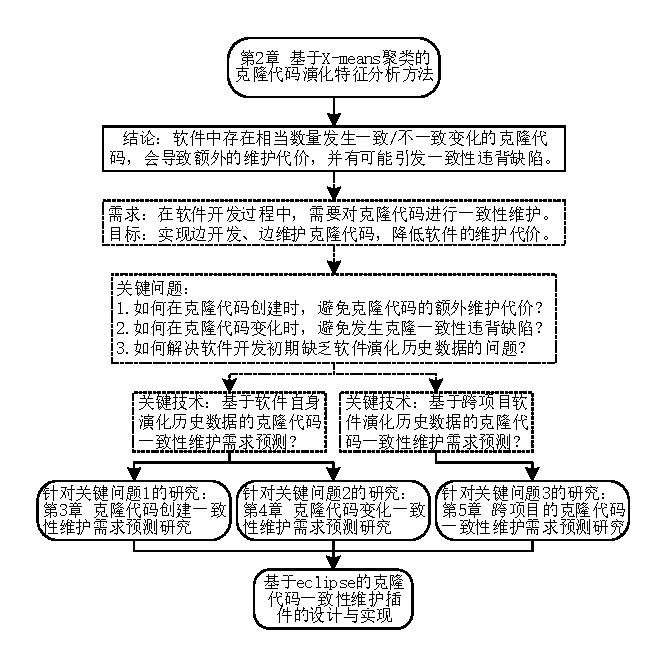
\includegraphics[width = 1.0\textwidth]{framework1.pdf}
\bicaption[framework1]{}{论文主要研究内容及其关系示意图}{Fig.$\!$}
{Main research contents and their relationship in the thesis}
%{Main Research Contents and Their Relationship in The Thesis}
\vspace{-1em}
\end{figure}

各章节研究内容安排如下:

第2章研究基于聚类的克隆代码演化特征分析方法,使用克隆演化特征帮助程序开发人员程序分析和理解克隆代码。首先,使用克隆检测工具检测系统中的克隆代码,并构建系统所有克隆代码的克隆家系用于描述克隆代码的演化过程。然后,从克隆片段、克隆组和克隆家系三个不同角度描述克隆代码及其演化过程并提取相应的度量值。最后,使用聚类分析方法聚类克隆代码并挖掘克隆代码演化特征,帮助开发人员理解克隆代码及其演化过程。

第3章研究基于贝叶斯网络的克隆代码创建时一致性维护需求预测方法,定义了克隆代码创建实例及其一致性维护需求。首先,通过检测系统的克隆代码并构建克隆家系收集系统中的克隆创建实例。然后,提取代码属性和上下文属性两组不同的度量值表示克隆创建实例的被复制和被粘贴的克隆代码。最后,使用贝叶斯网络预测克隆代码创建时一致性维护需求。

第4章研究基于贝叶斯网络的克隆代码变化时一致性维护需求预测方法,定义了克隆代码变化实例及其一致性维护需求。首先,通过检测系统的克隆代码并构建系统克隆家系收集系统中的克隆变化实例。然后,提取代码属性、上下文属性和演化属性三组不同的度量值用于表示克隆变化实例。最后,使用贝叶斯网络训练预测克隆代码变化时一致性维护需求。

第5章进行克隆代码一致性维护需求实证研究,统一了克隆代码创建和变化实例为克隆实例及其相应的克隆代码一致性维护需求。首先,检测系统的克隆代码并构建克隆家系收集所有的克隆代码实例,并使用不同的属性组表示克隆实例(与第3章和第4章相同)。然后,将克隆代码的一致性维护预测扩展到其它五种不同的机器学习方法中。最后,将克隆代码一致性维护需求预测与软件开发过程相结合,实现了一个eclipse插件可以实现边开发边预测克隆代码的一致性维护需求。

% !Mode:: "TeX:UTF-8" 

\BiChapter{图片的插入方法}{Methods of inserting figures}

\BiSection{研究生院的插图规范}{Figures inserting standard from graduate school}
图应有自明性。插图应与文字紧密配合,文图相符,内容正确。选图要力求精练,插图、照片应完整清晰。图中文字和数字等字号用宋体~5~号字。

机械工程图:采用第一角投影法,严格按照~GB4457---GB131-83《机械制图》标准规定。

数据流程图、程序流程图、系统流程图等按~GB1526-89~标准规定。

电气图:图形符号、文字符号等应符合附录~3~所列有关标准的规定。

流程图:必须采用结构化程序并正确运用流程框图。

对无规定符号的图形应采用该行业的常用画法。

坐标图的坐标线均用细实线,粗细不得超过图中曲线,有数字标注的坐标图,必须注明坐标单位。

照片图要求主题和主要显示部分的轮廓鲜明,便于制版。如用放大或缩小的复制品,必须清晰,反差适中。照片上应有表示目的物尺寸的标度。

引用文献图表必须标注出处。


\BiSubsection{图题及图中说明}{Captions and descriptions of figures}
每个图均应有图题(由图序和图名组成),图名在图序之后空一格排写。图序按章编排,如第~1~章第一个插图的图号为“图~1-1”等。
图题置于图下,硕士论文可只用中文书写,博士论文用中、英文两种文字居中书写,中文在上,要求中文用宋体~5~号字,英文用~Times New Roman 5~号字。有图注或其它说明时应置于图题之上。引用图应注明出处,在图题右上角加引用文献号。
图中若有分图时,分图题置于分图之下或图题之下,分图号用~a)、b)等表示。

图中各部分说明应采用中文(引用的外文图除外)或数字项号,各项文字说明置于图题之上(有分图题者,置于分图题之上)。

\BiSubsection{插图编排}{Layouts of illustrations}
插图之前,文中必须有关于本插图的提示,如“见图~1-1”、“如图~1-1~所示”等。插图与其图题为一个整体,不得拆开排写于两页。
插图处的该页空白不够排写该图整体时,则可将其后文字部分提前排写,将图移到次页。

\BiSection{\LaTeX~中推荐使用的图片格式}{Recommended figure format applied in \LaTeX}
在~\LaTeX~中应用最多的图片格式是~EPS(Encapsulated PostScript)格式,它是一种专用的打印机描述语言,常用于印刷或打印输出。
EPS~格式图片可通过多种方式生成,这里介绍一款功能强大的免费图片处理软件———\href{http://www.imagemagick.org/}{ImageMagick},
360~软件管家也提供此软件的下载。此软件可将其它格式图片转换为~EPS~格式图片,同时还可以锐化图片,使图片的局部清晰一些。

此软件对图片的格式转换操作都是在命令提示符(cmd.exe)中实现的,可以通过“开始$\to$运行$\to$输入~cmd$\to$回车”或
“开始$\to$程序$\to$附件$\to$命令提示符”找到它。在命令提示符下,首先采用“盘符命令”或“cd~命令”将当前目录改为待处理图片所在的目录,
在此目录下就可通过~convert~命令将图片转换为~EPS~格式,其命令的语法格式为

\noindent\verb|convert [可选参数] 原文件名.原扩展名 新文件名.eps|

\noindent 若~convert~命令中无可选参数,则将原来的图片格式直接转换为~EPS~格式,对图片不进行任何处理,这也是最常用的方法。
也可以选用可选参数,可选参数有很多选择,但最常用的有如下两个:

\verb|-sharpen radius{xsigma}|———此参数用来锐化图片,一般用在图片像素不高,需要提高图片清晰度的情况下。其中~radius~只能为整数,
它用来确定转换命令采取哪一种锐化算法,我们可以只取~radius~为~0;sigma~为所采取算法的锐化度,它的取值为~0.1--3~之间的任意一个浮点数,
数值越大,锐化程度也越大,通常取为~0.5--1~之间;x在参数中为分隔符。

\verb|-resize geometry|———此参数用来改变图片的大小,若图片的存储空间过大,可通过此命令缩小图片尺寸,但同时也将导致图片像素降低,
其具体用法请参见\href{http://www.imagemagick.org/script/command-line-options.php#resize}{-resize geometry的官方说明}。

除此之外,一些文字处理软件和科学计算软件也支持生成~EPS~格式的文件,请使用“另存为”功能查看某款软件是否能够将图片以~EPS~格式的形式保存。

\BiSection{单张图片的插入方法}{The method of inserting one single figure}
单张图片独自占一行的插入形式如图~\ref{golfer1}~所示。
\begin{figure}[htbp]
\centering
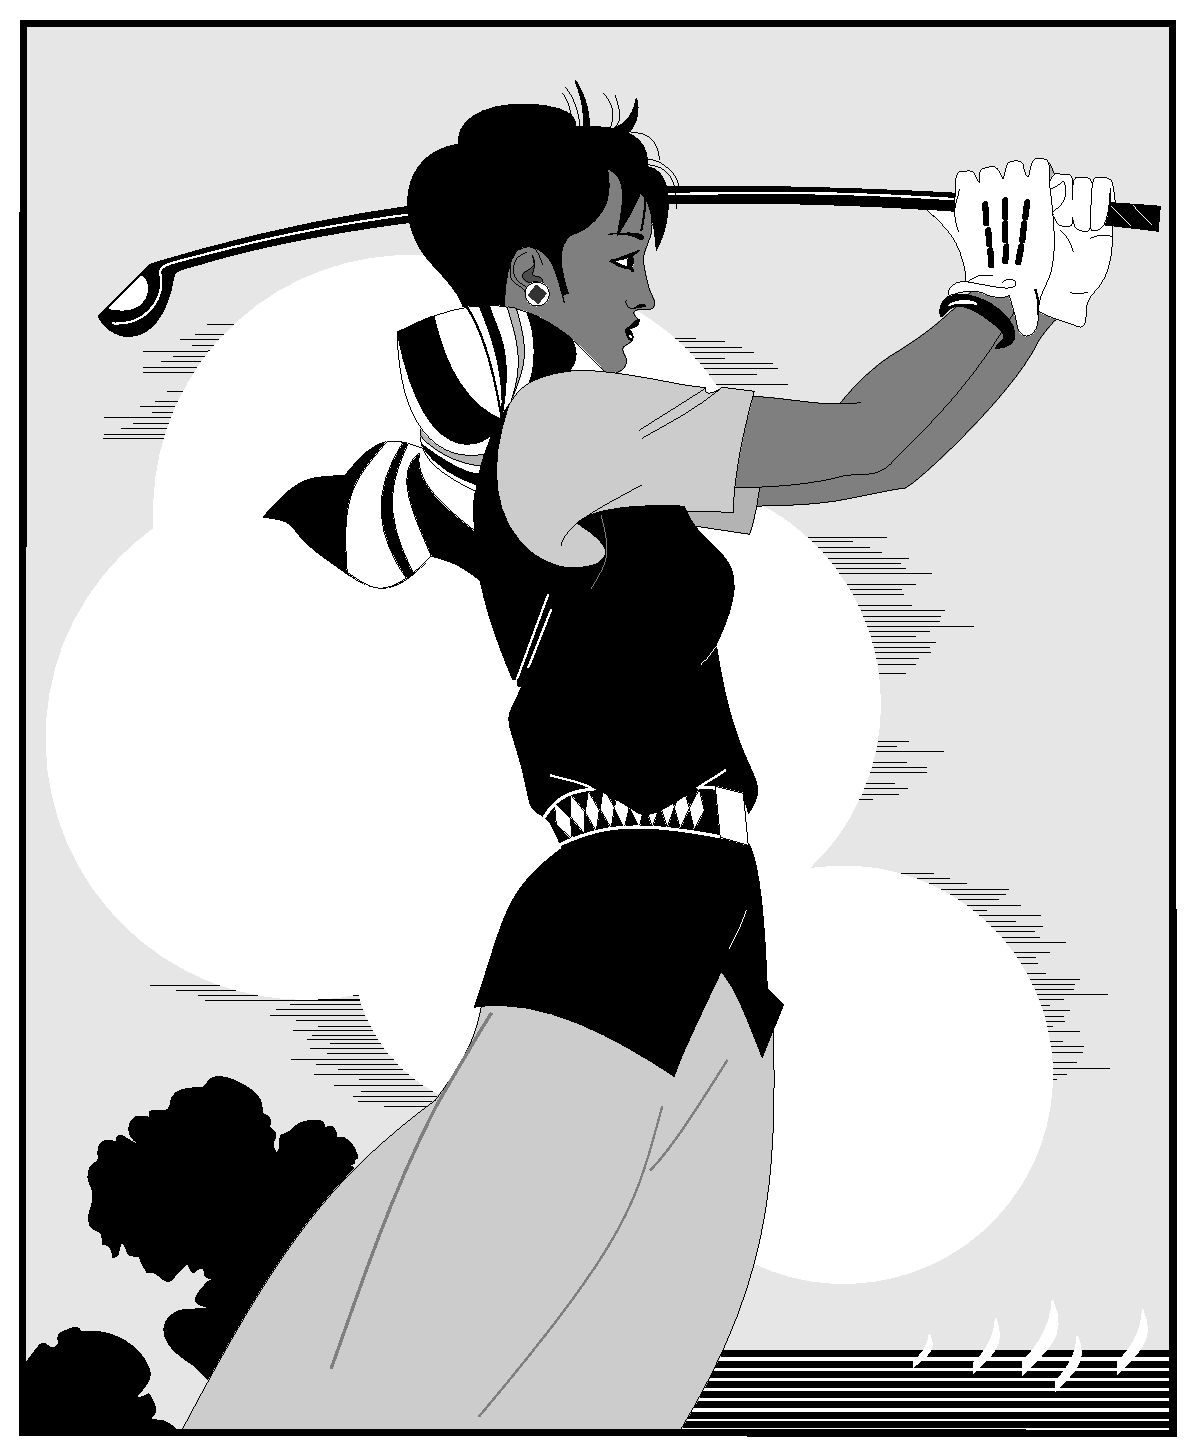
\includegraphics[width = 0.4\textwidth]{golfer}
\bicaption[golfer1]{}{打高尔夫球的人}{Fig.$\!$}{The person playing golf}\vspace{-1em}
\end{figure}

其插入图片的代码及其说明如下。
\vspace{1em}\noindent\hrule
\begin{lstlisting}
\begin{figure}[htbp]
\centering
\includegraphics[width=0.4\textwidth]{文件名(.eps)}
\bicaption[标签名(英文)]{}{中文标题}{Fig.$\!$}
          {English caption (首字母大写)}\vspace{-1em}
\end{figure}
\end{lstlisting}
\noindent\hrule
\begin{lstlisting}
figure环境的可选参数[htbp]表示浮动图形所放置的位置,h (here)表示当前位置,t (top)表示页芯顶部,b (bottom)表示页芯底部,p (page)表示单独一页。在word等软件中,图片通常插入到当前位置,如果当前页的剩余空间不够,图片将被移动到下一页,当前页就会出现很大的空白,其人工调整工作非常不便。由LaTeX提供的浮动图片功能,总是会按h->t->b->p的次序处理选项中的字母,自动调整图片的位置,大大减轻了工作量。
\centering命令将后续内容转换成每行皆居中的格式。
“\includegraphics”的可选参数用来设置图片插入文中的水平宽度,一般表示为正文宽度(\textwidth)的倍数。
\bicaption命令的使用需要调用ccaption宏包,它可以为图片或表格插入双语标题(博士学位论文要求),可选参数“标签名”为英文形式,一般不以图片或表格的数字顺序作为标签,而应包含一定的图片或表格信息,以便于文中引用(若图片、表格、公式、章节和参考文献等在文中出现的先后顺序发生了变化,其标注序号及其文中引用序号也会跟着发生变化,这一点是word等软件所不能做到的)。第4个参数中的“$\!$”表示-1/6个空铅宽度,这样可以缩小Fig.和Table与后面数字序号之间的水平距离。另外,图题或表题并不会因为分页而与图片或表格体分置于两页,章节等各级标题也不会置于某页的最底部,LaTeX系统会自动调整它们在正文中的位置,这也是word等软件所无法匹敌的。
注:硕士学位论文的图表只需要插入中文标题,因此需将\bicaption一句命令替换为如下两条命令(下同):
\caption{中文标题}
\label{标签名(英文)}
\vspace将产生一定高度的竖直空白,必选参数为负值表示将后续文字位置向上提升,参数值可自行调整。em为长度单位,相当于大写字母M的宽度。
引用方法:“见图~\ref{标签名(英文)}”、“如图~\ref{标签名(英文)}~所示”等。
\end{lstlisting}
\noindent\hrule\vspace{1em}
若需要将~2~张及以上的图片并排插入到一行中,则需要采用\verb|minipage|环境,如图~\ref{golfer2}~和图~\ref{golfer3}~所示。
\begin{figure}[htbp]
\centering
\begin{minipage}{0.4\textwidth}
\centering
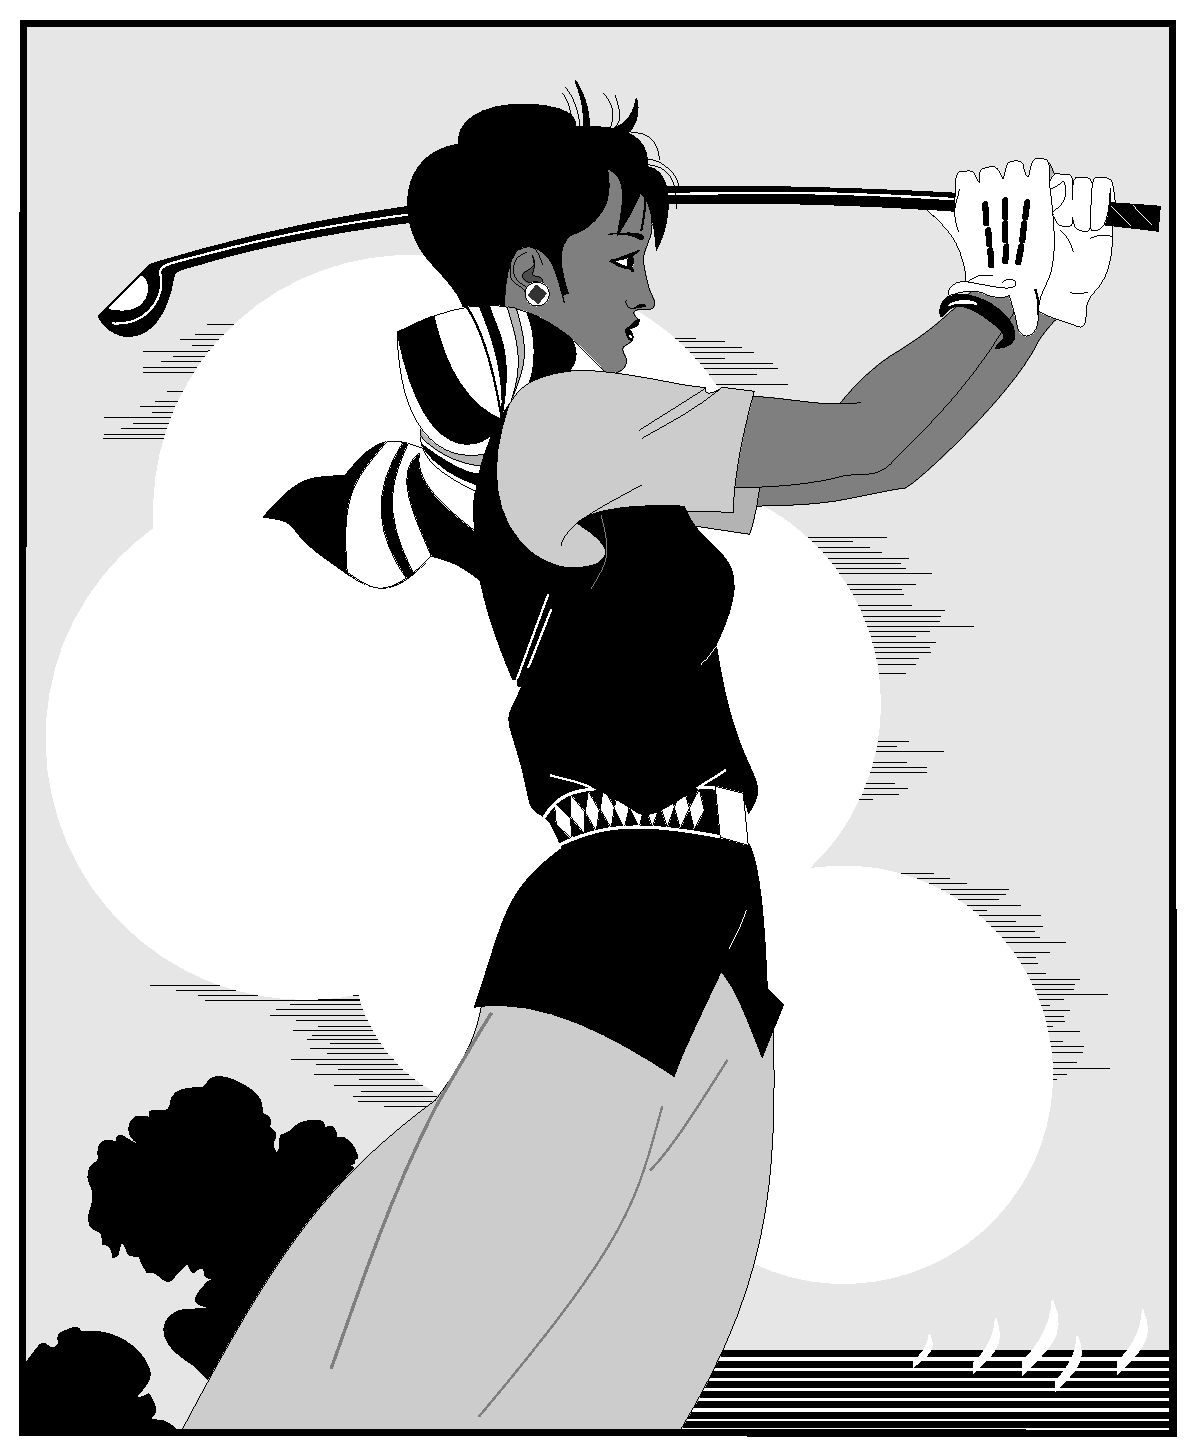
\includegraphics[width=\textwidth]{golfer}
\bicaption[golfer2]{}{打高尔夫球的人}{Fig.$\!$}{The person playing golf}
\end{minipage}
\begin{minipage}{0.4\textwidth}
\centering
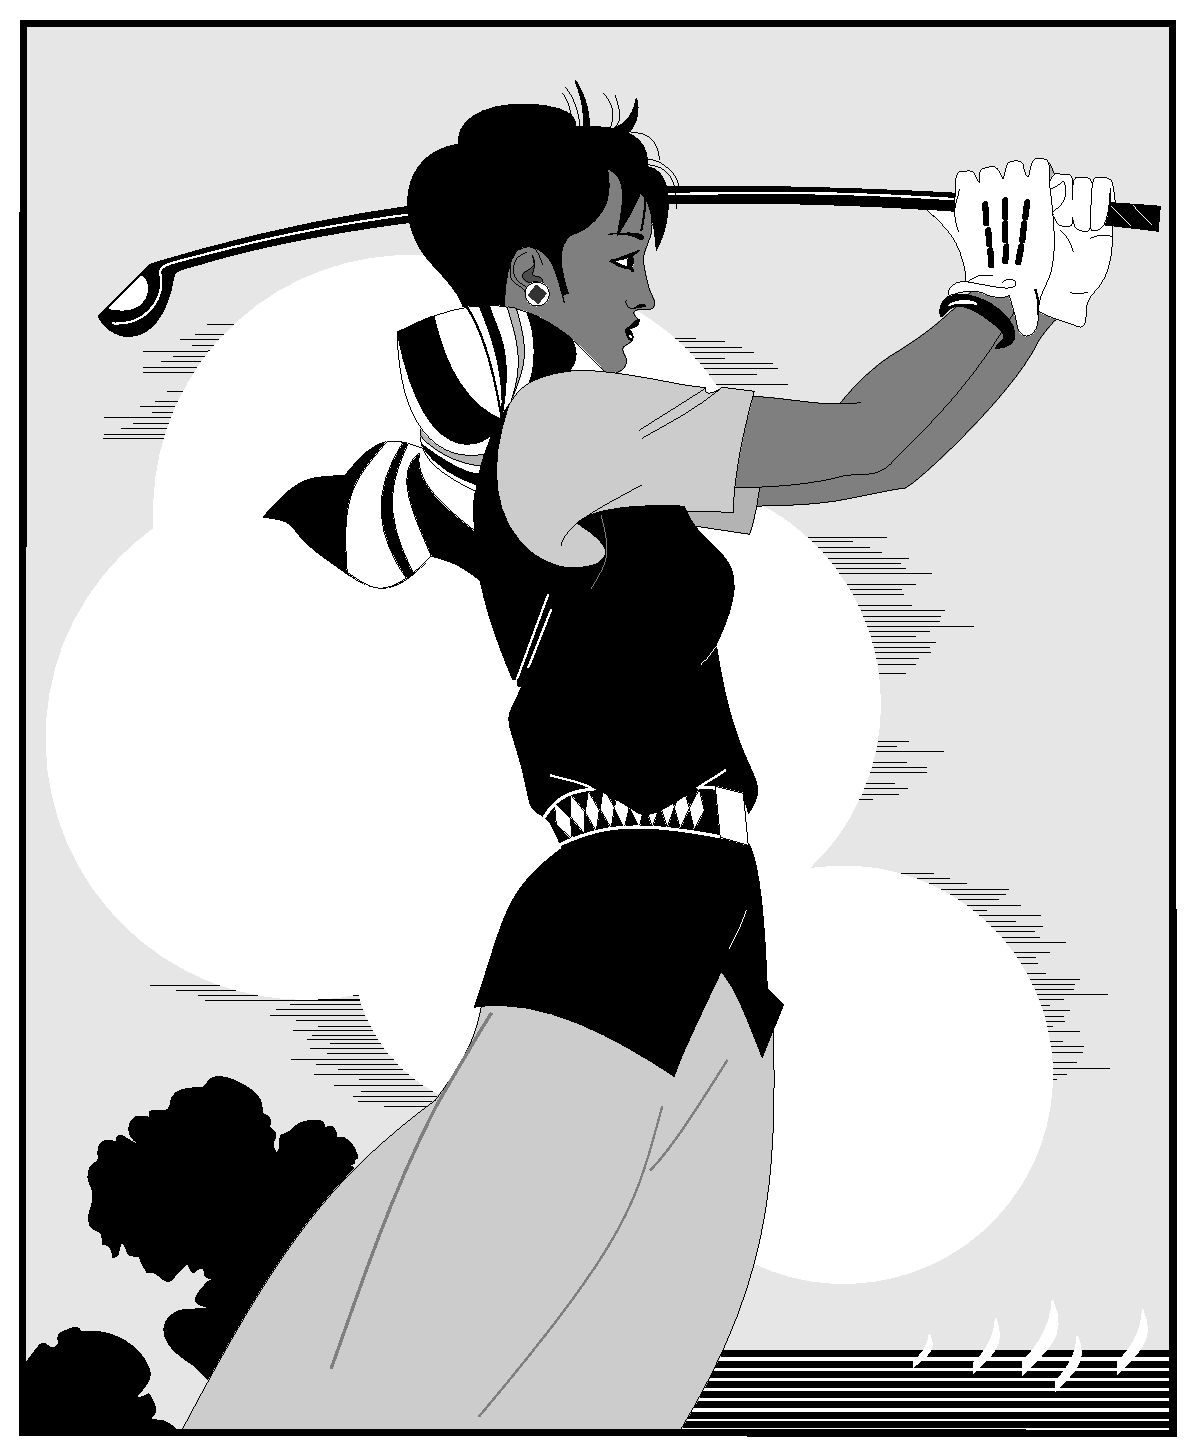
\includegraphics[width=\textwidth]{golfer}
\bicaption[golfer3]{}{打高尔夫球的人}{Fig.$\!$}{The person playing golf}
\end{minipage}\vspace{-1em}
\end{figure}

其代码如下所示。
\vspace{1em}\noindent\hrule
\begin{lstlisting}
\begin{figure}[htbp]
\centering
\begin{minipage}{0.4\textwidth}
\centering
\includegraphics[width=\textwidth]{文件名}
\bicaption[标签名]{}{中文标题}{Fig.$\!$}
          {English caption}
\end{minipage}
\begin{minipage}{0.4\textwidth}
\centering
\includegraphics[width=\textwidth]{文件名}
\bicaption[标签名]{}{中文标题}{Fig.$\!$}
          {English caption}
\end{minipage}\vspace{-1em}
\end{figure}
\end{lstlisting}
\noindent\hrule
\begin{lstlisting}
minipage环境的必选参数用来设置小页的宽度,若需要在一行中插入n个等宽图片,则每个小页的宽度应略小于(1/n)\textwidth。
\end{lstlisting}
\noindent\hrule

\BiSection{具有子图的图片插入方法}{The method of inserting figures with subfigures}

图中若含有子图时,需要调用~subfigure~宏包。博士学位论文规范要求不止总图的标题为中英文形式,其各个子图也应具有中英文形式的标题。
然而~ccaption~宏包却无法实现子图的中英文标题功能,这里采用对\verb|\subfigure|命令进行嵌套的方法来实现子图的中英文标题功能,如图~\ref{golfer4}~所示。

\begin{figure}[htbp]
\centering
\subfigure{\label{golfer41}}\addtocounter{subfigure}{-2}
\subfigure[The person playing golf]{\subfigure[打高尔夫球的人~1]{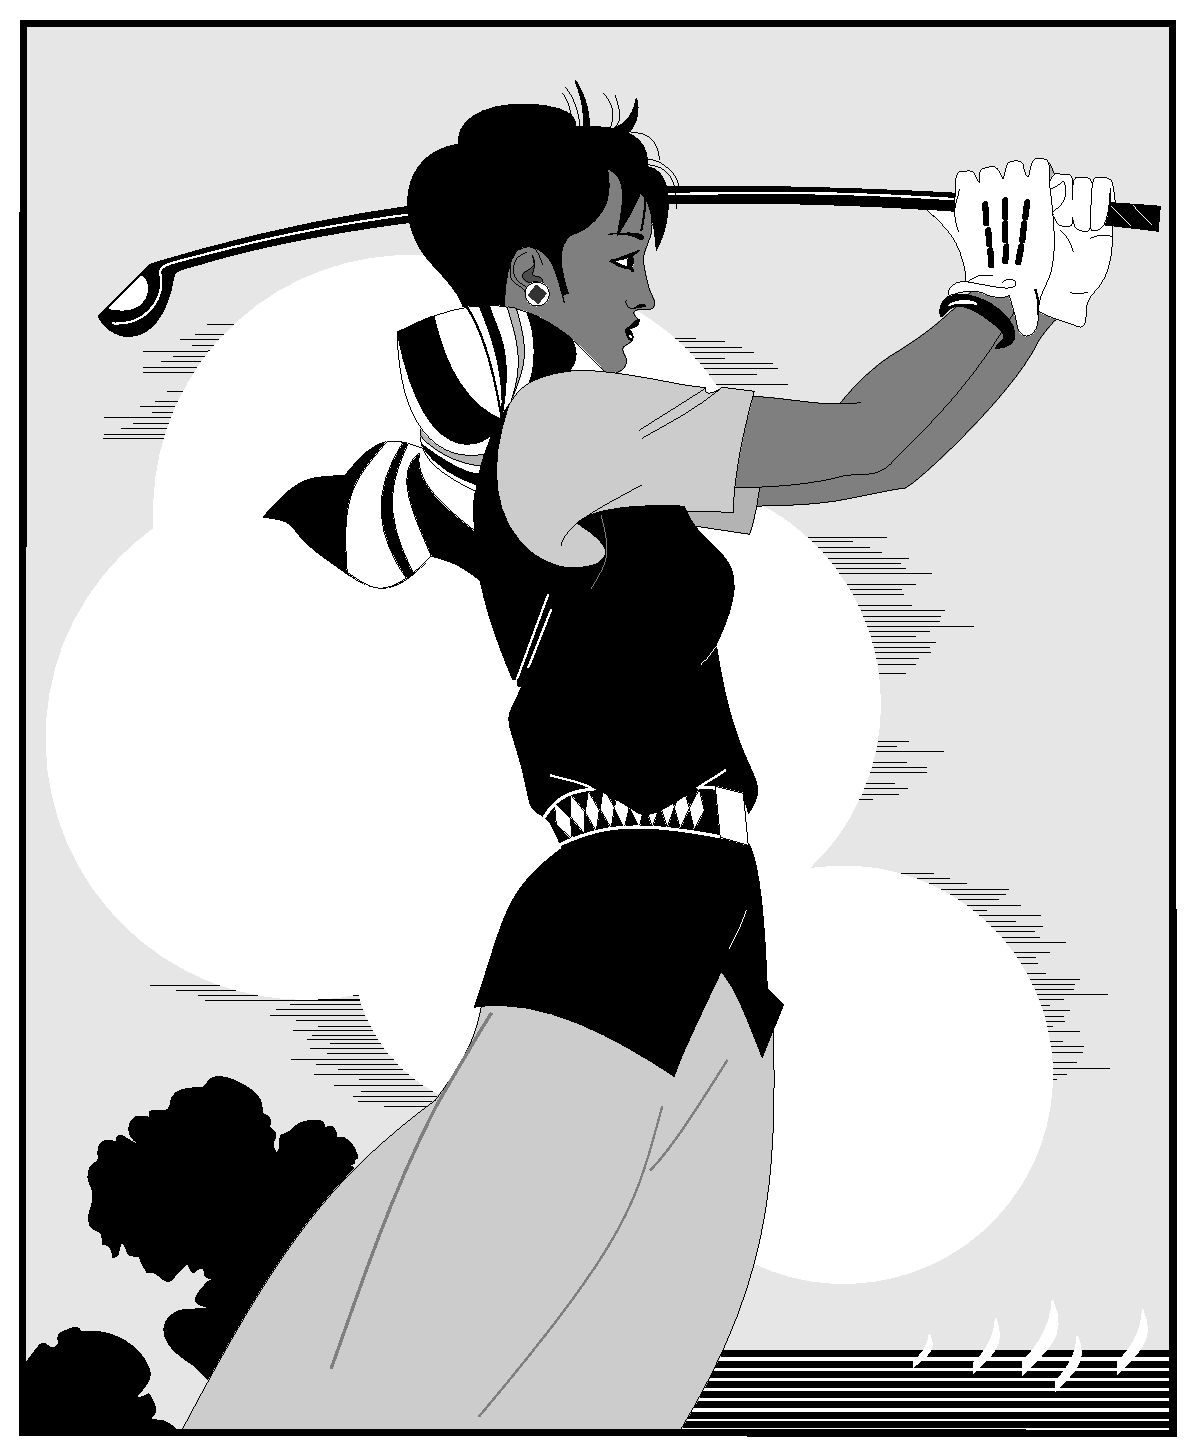
\includegraphics[width=0.4\textwidth]{golfer}}}
\subfigure{\label{golfer42}}\addtocounter{subfigure}{-2}
\subfigure[The person playing golf]{\subfigure[打高尔夫球的人~2]{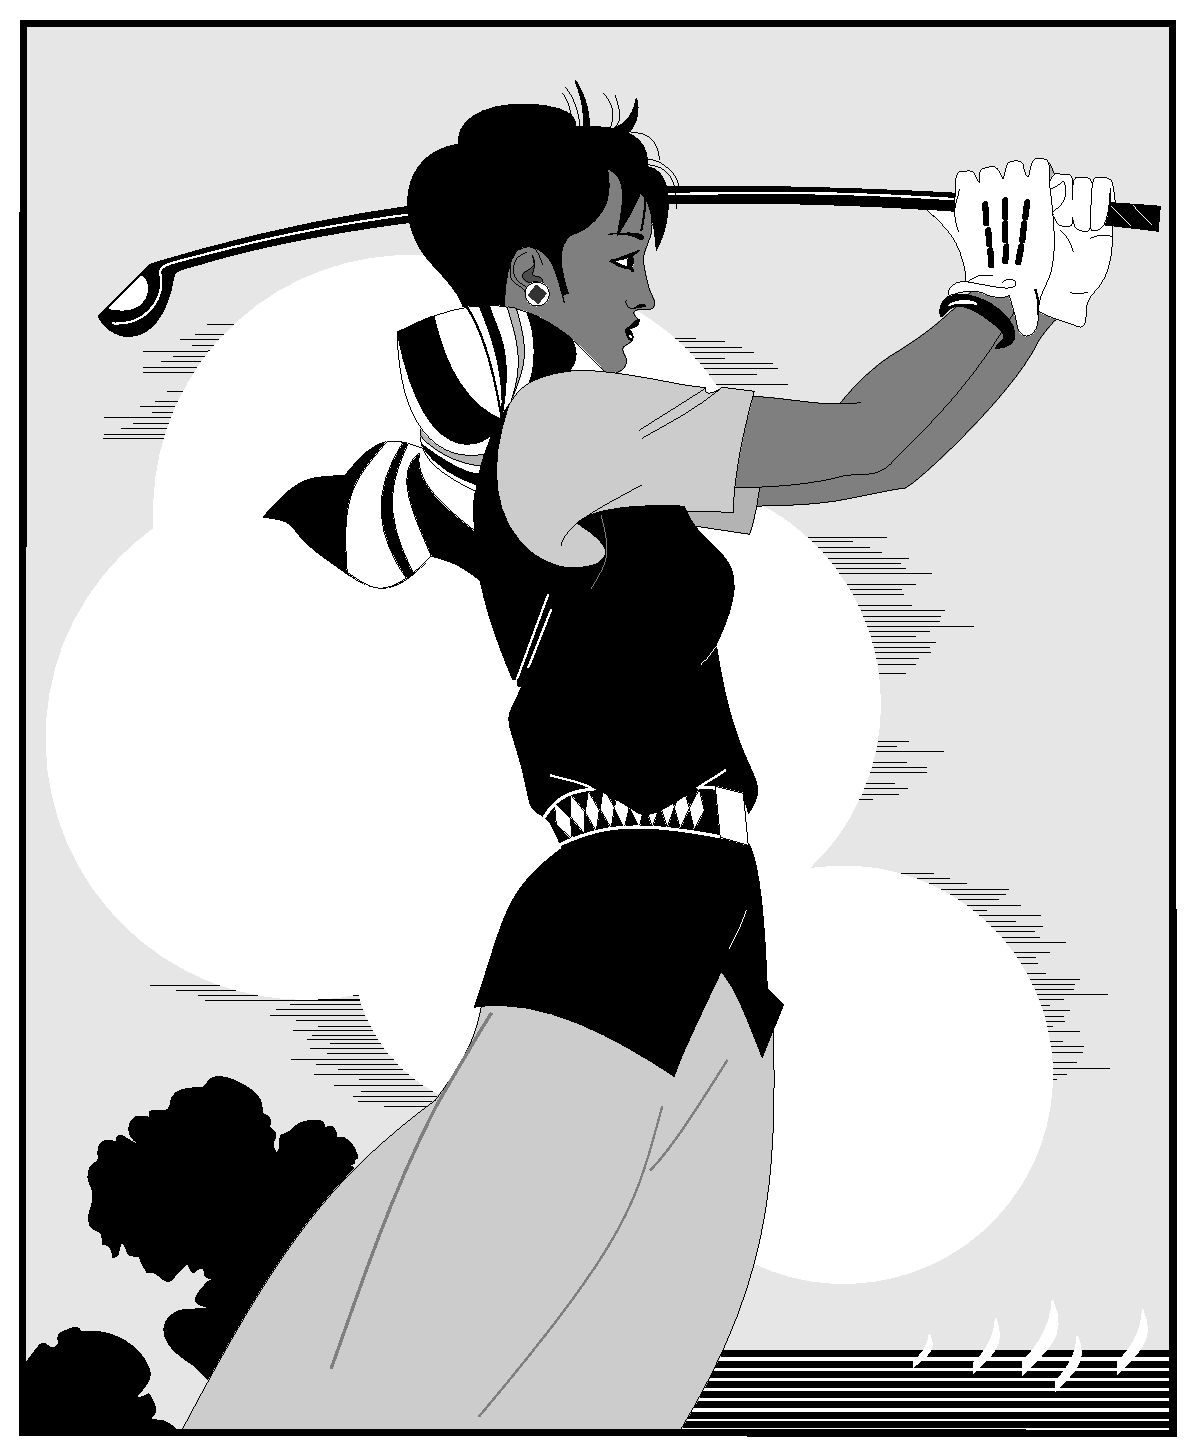
\includegraphics[width=0.4\textwidth]{golfer}}}
\bicaption[golfer4]{}{打高尔夫球的人}{Fig.$\!$}{The person playing golf}\vspace{-1em}
\end{figure}

其代码及其说明如下。
\vspace{1em}\noindent\hrule
\begin{lstlisting}
\begin{figure}[htbp]
\centering
\subfigure{\label{第1个子图标签名}}\addtocounter{subfigure}{-2}
\subfigure[The 1st subfigure caption]{\subfigure[第1个子图标题]
          {\includegraphics[width=0.4\textwidth]{文件名}}}
\subfigure{\label{第2个子图标签名}}\addtocounter{subfigure}{-2}
\subfigure[The 2nd subfigure caption]{\subfigure[第2个子图标题]
          {\includegraphics[width=0.4\textwidth]{文件名}}}
\bicaption[总标签名]{}{中文总标题}{Fig.$\!$}{The total caption}
\vspace{-1em}
\end{figure}
\end{lstlisting}
\noindent\hrule
\begin{lstlisting}
\addtocounter把指定的值加到计数器上,这里是对subfigure计数器进行减2操作。这是因为每插入1个子图,就调用3次\subfigure命令,第1次调用\subfigure命令用来生成紧随其后所插入子图的标签,而之后的双层嵌套调用\subfigure命令用来插入子图并生成该子图的中英文标题。因此,每插入1张子图,subfigure计数器的值就自动加3,为了使得子图的序号能每次加1,则需在每插入1张子图前手动把subfigure计数器的值减2。
\subfigure命令的双层嵌套使用可用来生成中英文标题,其内层\subfigure命令用来插入子图并生成中文标题,外层\subfigure命令将插入的子图和中文标题作为一个整体,生成这个整体的英文标题,因此英文标题会置于中文标题的下面。
硕士学位论文只需要中文标题,其代码如下:
\begin{figure}[htbp]
\centering
\subfigure[第1个子图标题\label{第1个子图标签名}]
          {\includegraphics[width=0.4\textwidth]{文件名}}
\subfigure[第2个子图标题\label{第2个子图标签名}]
          {\includegraphics[width=0.4\textwidth]{文件名}}
\caption{中文总标题}\label{总标签名}
\vspace{-1em}
\end{figure}
引用方法:总图的引用方法同本章第1节,子图的引用方法用\ref{第n个子图标签名}来代替。
\end{lstlisting}
\noindent\hrule\vspace{1em}

子图的引用示例:如图~\ref{golfer41}~和图~\ref{golfer42}~所示。

若想获得插图方法的更多信息,请参见网络上的~\href{ftp://ftp.tex.ac.uk/tex-archive/info/epslatex.pdf}{Using Imported Graphics in \LaTeX and pdf\LaTeX}~文档。 

% !Mode:: "TeX:UTF-8" 

\BiChapter{表格的绘制方法}{Methods of drawing tables}
\BiSection{研究生院的绘表规范}{Tables drawing standard from graduate school}

表应有自明性。表格不加左、右边线。表的编排建议采用国际通行的三线表。表中文字用宋体~5~号字。

每个表格均应有表题(由表序和表名组成)。表序一般按章编排,如第~1~章第一个插表的序号为“表~1-1”等。表序与表名之间空一格,
表名中不允许使用标点符号,表名后不加标点。表题置于表上,硕士学位论文只用中文,博士学位论文用中、英文两种文字居中排写,
中文在上,要求中文用宋体~5~号字,英文用新罗马字体~5~号字。

表头设计应简单明了,尽量不用斜线。表头中可采用化学符号或物理量符号。

全表如用同一单位,则将单位符号移至表头右上角,加圆括号。
表中数据应准确无误,书写清楚。数字空缺的格内加横线“-”(占~2~个数字宽度)。表内文字或数字上、下或左、右相同时,
采用通栏处理方式,不允许用“〃”、“同上”之类的写法。

表内文字说明,起行空一格、转行顶格、句末不加标点。

如某个表需要转页接排,在随后的各页上应重复表的编号。编号后加“(续表)”,表题可省略。续表应重复表头。

\BiSection{普通表格的绘制方法}{Methods of drawing normal tables}

表格应具有三线表格式,因此需要调用~booktabs~宏包,其标准格式如表~\ref{table1}~所示。
\begin{table}[htbp]
\bicaption[table1]{}{符合研究生院绘图规范的表格}{Table$\!$}{Table in agreement of the standard from graduate school}
\vspace{0.5em}\centering\wuhao
\begin{tabular}{ccccc}
\toprule[1.5pt]
$D$(in) & $P_u$(lbs) & $u_u$(in) & $\beta$ & $G_f$(psi.in)\\
\midrule[1pt]
 5 & 269.8 & 0.000674 & 1.79 & 0.04089\\
10 & 421.0 & 0.001035 & 3.59 & 0.04089\\
20 & 640.2 & 0.001565 & 7.18 & 0.04089\\
\bottomrule[1.5pt]
\end{tabular}
\end{table}

其绘制表格的代码及其说明如下。
\vspace{1em}\noindent\hrule
\begin{lstlisting}
\begin{table}[htbp]
\bicaption[标签名]{}{中文标题}{Table$\!$}{English caption}
\vspace{0.5em}\centering\wuhao
\begin{tabular}{cc...c}
\toprule[1.5pt]
表头第1个格   & 表头第2个格   & ... & 表头第n个格  \\
\midrule[1pt]
表中数据(1,1) & 表中数据(1,2) & ... & 表中数据(1,n)\\
表中数据(2,1) & 表中数据(2,2) & ... & 表中数据(2,n)\\
...................................................\\
表中数据(m,1) & 表中数据(m,2) & ... & 表中数据(m,n)\\
\bottomrule[1.5pt]
\end{tabular}
\end{table}
\end{lstlisting}
\noindent\hrule
\begin{lstlisting}
table环境是一个将表格嵌入文本的浮动环境。
\wuhao命令将表格的字号设置为五号字(10.5pt),在绘制表格结束退出时,不需要将字号再改回为\xiaosi,正文字号默认为小四号字(12pt)。
tabular环境的必选参数由每列对应一个格式字符所组成:c表示居中,l表示左对齐,r表示右对齐,其总个数应与表的列数相同。此外,@{文本}可以出现在任意两个上述的列格式之间,其中的文本将被插入每一行的同一位置。表格的各行以\\分隔,同一行的各列则以&分隔。
\toprule、\midrule和\bottomrule三个命令是由booktabs宏包提供的,其中\toprule和\bottomrule分别用来绘制表格的第一条(表格最顶部)和第三条(表格最底部)水平线,\midrule用来绘制第二条(表头之下)水平线,且第一条和第三条水平线的线宽为1.5pt,第二条水平线的线宽为1pt。
引用方法:“如表~\ref{标签名}~所示”。
\end{lstlisting}
\noindent\hrule

\BiSection{长表格的绘制方法}{Methods of drawing long tables}

长表格是当表格在当前页排不下而需要转页接排的情况下所采用的一种表格环境。若长表格仍按照普通表格的绘制方法来获得,
其所使用的\verb|table|浮动环境无法实现表格的换页接排功能,表格下方过长部分会排在表格第1页的页脚以下。为了能够实现长表格的转页接排功能,
需要调用~longtable~宏包,由于长表格是跨页的文本内容,因此只需要单独的\verb|longtable|环境,所绘制的长表格的格式如表~\ref{table2}~所示。

此长表格~\ref{table2}~第~2~页的标题“编号(续表)”和表头是通过代码自动添加上去的,无需人工添加,若表格在页面中的竖直位置发生了变化,长表格在第~2~页
及之后各页的标题和表头位置能够始终处于各页的最顶部,也无需人工调整,\LaTeX~系统的这一优点是~word~等软件所无法比拟的。

\wuhao\begin{longtable}{ccc}
\longbionenumcaption{}{中国省级行政单位一览\label{table2}}{Table$\!$}{}{Overview of the provincial administrative unit of China} \vspace{0.5em}\\
\toprule[1.5pt] 名称 & 简称 & 省会或首府  \\ \midrule[1pt]
\endfirsthead
\multicolumn{3}{r}{表~\thetable(续表)}\vspace{0.5em}\\
\toprule[1.5pt] 名称 & 简称 & 省会或首府  \\ \midrule[1pt]
\endhead
\bottomrule[1.5pt]
\endfoot
北京市 & 京 & 北京\\
天津市 & 津 & 天津\\
河北省 & 冀 & 石家庄市\\
山西省 & 晋 & 太原市\\
内蒙古自治区 & 蒙 & 呼和浩特市\\
辽宁省 & 辽 & 沈阳市\\
吉林省 & 吉 & 长春市\\
黑龙江省 & 黑 & 哈尔滨市\\
上海市 & 沪/申 & 上海\\
江苏省 & 苏 & 南京市\\
浙江省 & 浙 & 杭州市\\
安徽省 & 皖 & 合肥市\\
福建省 & 闽 & 福州市\\
江西省 & 赣 & 南昌市\\
山东省 & 鲁 & 济南市\\
河南省 & 豫 & 郑州市\\
湖北省 & 鄂 & 武汉市\\
湖南省 & 湘 & 长沙市\\
广东省 & 粤 & 广州市\\
广西壮族自治区 & 桂 & 南宁市\\
海南省 & 琼 & 海口市\\
重庆市 & 渝 & 重庆\\
四川省 & 川/蜀 & 成都市\\
贵州省 & 黔/贵 & 贵阳市\\
云南省 & 云/滇 & 昆明市\\
西藏自治区 & 藏 & 拉萨市\\
陕西省 & 陕/秦 & 西安市\\
甘肃省 & 甘/陇 & 兰州市\\
青海省 & 青 & 西宁市\\
宁夏回族自治区 & 宁 & 银川市\\
新疆维吾尔自治区 & 新 & 乌鲁木齐市\\
香港特别行政区 & 港 & 香港\\
澳门特别行政区 & 澳 & 澳门\\
台湾省 & 台 & 台北市\\
\end{longtable}\xiaosi

绘制长表格的代码及其说明如下。
\vspace{1em}\noindent\hrule
\begin{lstlisting}

\wuhao\begin{longtable}{cc...c}
\longbionenumcaption{}{中文标题\label{标签名}}{Table$\!$}
                    {}{English caption}\vspace{0.5em}\\
\toprule[1.5pt] 表头第1个格 & 表头第2个格 & ... & 表头第n个格\\ \midrule[1pt]
\endfirsthead
\multicolumn{n}{r}{表~\thetable(续表)}\vspace{0.5em}\\
\toprule[1.5pt] 表头第1个格 & 表头第2个格 & ... & 表头第n个格\\ \midrule[1pt]
\endhead
\bottomrule[1.5pt]
\endfoot
表中数据(1,1) & 表中数据(1,2) & ... & 表中数据(1,n)\\
表中数据(2,1) & 表中数据(2,2) & ... & 表中数据(2,n)\\
...................................................\\
表中数据(m,1) & 表中数据(m,2) & ... & 表中数据(m,n)\\
\end{longtable}\xiaosi
\end{lstlisting}
\noindent\hrule
\begin{lstlisting}
在绘制长表格的前面留出一个空白行,并在第2行的一开始全局定义长表格的字号为五号字,这样能够保证长表格之前段落的行距保持不变。在绘制长表格结束后,需要\xiaosi命令重新将字号改为小四号字。
长表格的中英文标题是通过ccaption宏包的\longbionenumcaption命令得到的。
\endhead之前的文字描述的是第2页及其之后各页的标题或表头;\endfirsthead之前的文字描述的是第1页的标题和表头,若无此命令,则第1页的表头和标题由\endhead命令确定;同理,\endfoot之前的文字描述的是除最后一页之外每页的表格底部内容;\endlastfoot之前的文字描述的是最后一页的表格底部内容,若无此命令,则最后一页的表格底部内容由\endfoot命令确定;由于规范中长表格每页底部内容均相同(水平粗线),因此模板中没有用到\endlastfoot命令。
注:硕士学位论文的长表格只需要插入中文标题,因此需将\longbionenumcaption一句命令替换为如下两条命令 :
\caption{中文标题}
\label{标签名}
\end{lstlisting}
\noindent\hrule

\BiSection{列宽可调表格的绘制方法}{Methods of drawing tables with adjustable-width columns}
论文中能用到列宽可调表格的情况共有两种,一种是当插入的表格某一单元格内容过长以至于一行放不下的情况,
另一种是当对公式中首次出现的物理量符号进行注释的情况,这两种情况都需要调用~tabularx~宏包。下面将分别对这两种情况下可调表格的绘制方法进行阐述。
\BiSubsection{表格内某单元格内容过长的情况}{The condition when the contents in some cells of tables are too long}
首先给出这种情况下的一个例子如表~\ref{table3}~所示。
\begin{table}[htbp]
  \centering
\bicaption[table3]{}{最小的三个正整数的英文表示法}{Table$\!$}{The English construction of the smallest three positive integral numbers}\vspace{0.5em}\wuhao
\begin{tabularx}{0.7\textwidth}{llX}
\toprule[1.5pt]
Value & Name & Alternate names, and names for sets of the given size\\\midrule[1pt]
1 & One & ace, single, singleton, unary, unit, unity\\
2 & Two & binary, brace, couple, couplet, distich, deuce, double, doubleton, duad, duality, duet, duo, dyad, pair, snake eyes, span, twain, twosome, yoke\\
3 & Three & deuce-ace, leash, set, tercet, ternary, ternion, terzetto, threesome, tierce, trey, triad, trine, trinity, trio, triplet, troika, hat-trick\\\bottomrule[1.5pt]
\end{tabularx}
\end{table}

绘制这种表格的代码及其说明如下。
\vspace{1em}\noindent\hrule
\begin{lstlisting}
\begin{table}[htbp]
\bicaption[标签名]{}{中文标题}{Table$\!$}{English caption}
\vspace{0.5em}\wuhao
\begin{tabularx}{\textwidth}{l...X...l}
\toprule[1.5pt]
表头第1个格   & ... & 表头第X个格   & ... & 表头第n个格  \\
\midrule[1pt]
表中数据(1,1) & ... & 表中数据(1,X) & ... & 表中数据(1,n)\\
表中数据(2,1) & ... & 表中数据(2,X) & ... & 表中数据(2,n)\\
.........................................................\\
表中数据(m,1) & ... & 表中数据(m,X) & ... & 表中数据(m,n)\\
\bottomrule[1.5pt]
\end{tabularx}
\end{table}
\end{lstlisting}
\noindent\hrule

\begin{lstlisting}

tabularx环境共有两个必选参数:第1个参数用来确定表格的总宽度,这里取为排版表格能达到的最大宽度——正文宽度\textwidth;第2个参数用来确定每列格式,其中标为X的项表示该列的宽度可调,其宽度值由表格总宽度确定。
标为X的列一般选为单元格内容过长而无法置于一行的列,这样使得该列内容能够根据表格总宽度自动分行。若列格式中存在不止一个X项,则这些标为X的列的列宽相同,因此,一般不将内容较短的列设为X。
标为X的列均为左对齐,因此其余列一般选为l(左对齐),这样可使得表格美观,但也可以选为c或r。

\end{lstlisting}

\noindent\hrule

\BiSubsection{对物理量符号进行注释的情况}{The condition when physical symbols need to be annotated}

为使得对公式中物理量符号注释的转行与破折号“———”后第一个字对齐,此处最好采用表格环境。此表格无任何线条,左对齐,
且在破折号处对齐,一共有“式中”二字、物理量符号和注释三列,表格的总宽度可选为文本宽度,因此应该采用\verb|tabularx|环境。
由\verb|tabularx|环境生成的对公式中物理量符号进行注释的公式如式(\ref{eq:1})所示。

\begin{equation}\label{eq:1}
\ddot{\boldsymbol{\rho}}-\frac{\mu}{R_{t}^{3}}\left(3\mathbf{R_{t}}\frac{\mathbf{R_{t}\rho}}{R_{t}^{2}}-\boldsymbol{\rho}\right)=\mathbf{a}
\end{equation}
\begin{tabularx}{\textwidth}{@{}l@{\quad}r@{———}X@{}}
式中& $\boldsymbol{\rho}$ &追踪飞行器与目标飞行器之间的相对位置矢量;\\
&  $\boldsymbol{\ddot{\rho}}$&追踪飞行器与目标飞行器之间的相对加速度;\\
&  $\mathbf{a}$   &推力所产生的加速度;\\
&  $\mathbf{R_t}$ & 目标飞行器在惯性坐标系中的位置矢量;\\
&  $\omega_{t}$ & 目标飞行器的轨道角速度;\\
&  $\mathbf{g}$ & 重力加速度,$=\frac{\mu}{R_{t}^{3}}\left(
3\mathbf{R_{t}}\frac{\mathbf{R_{t}\rho}}{R_{t}^{2}}-\boldsymbol{\rho}\right)=\omega_{t}^{2}\frac{R_{t}}{p}\left(
3\mathbf{R_{t}}\frac{\mathbf{R_{t}\rho}}{R_{t}^{2}}-\boldsymbol{\rho}\right)$,这里~$p$~是目标飞行器的轨道半通径。
\end{tabularx}\vspace{\wordsep}

其中生成注释部分的代码及其说明如下。
\vspace{1em}\noindent\hrule
\begin{lstlisting}
\begin{tabularx}{\textwidth}{@{}l@{\quad}r@{— — —}X@{}}
式中 & symbol-1 & symbol-1的注释内容;\\
     & symbol-2 & symbol-2的注释内容;\\
     .............................;\\
     & symbol-m & symbol-m的注释内容。
\end{tabularx}\vspace{\wordsep}
\end{lstlisting}
\noindent\hrule
\begin{lstlisting}
tabularx环境的第1个参数选为正文宽度,第2个参数里面各个符号的意义为:
    第1个@{}表示在“式中”二字左侧不插入任何文本,“式中”二字能够在正文中左对齐,若无此项,则“式中”二字左侧会留出一定的空白;
    @{\quad}表示在“式中”和物理量符号间插入一个空铅宽度的空白;
    @{— — —}实现插入破折号的功能,它由三个1/2的中文破折号构成;
    第2个@{}表示在注释内容靠近正文右边界的地方能够实现右对齐。
\end{lstlisting}
\noindent\hrule\vspace{1em}
由此方法生成的注释内容应紧邻待注释公式并置于其下方,因此不能将代码放入\verb|table|浮动环境中。但此方法不能实现自动转页接排,
可能会在当前页剩余空间不够时,全部移动到下一页而导致当前页出现很大空白。因此在需要转页处理时,还请您手动将需要转页的代码放入一个
新的\verb|tabularx|环境中,将原来的一个\verb|tabularx|环境拆分为两个\verb|tabularx|环境。

若想获得绘制表格的更多信息,请参见网络上的~\href{http://www.tug.org/pracjourn/2007-1/mori/}{Tables in \LaTeXe: Packages and Methods}~文档。 

% !Mode:: "TeX:UTF-8" 

\BiChapter{数学公式的输入方法}{Input methods of equations}
\BiSection{研究生院的公式规范}{Equations typesetting standard from graduate school}
论文中的公式应另起行,原则上应居中书写,与周围文字留有足够的空间区分开。
若公式前有文字(如“解”、“假定”等),文字空两格写,公式仍居中写。公式末不加标点。

公式应标注序号,并将序号置于括号内。 公式序号按章编排,如第~1~章第一个公式序号为“(1-1)”。公式的序号右端对齐。

公式较长时最好在等号“=”处转行,如难实现,则可在~$+$、$-$、$\times$、$\div$~运算符号处转行,转行时运算符号仅书写于转行式前,不重复书写。

文中引用公式时,一般用“见式~(1-1)”或“由公式~(1-1)”。

公式中用斜线表示“除”的关系时应采用括号,以免含糊不清,如~$a/(b\cos x)$。通常“乘”的关系在前,如~$a\cos x/b$而不写成~$(a/b)\cos x$。

不能用文字形式表示等式,如:$\textnormal{刚度}=\frac{{\textnormal{受力}}}{{\textnormal{受力方向的位移}}}$。

\textbf{对于数学公式的输入方法,网络上有一个比较全面权威的文档~\href{http://tug.ctan.org/cgi-bin/ctanPackageInformation.py?id=voss-mathmode}{Math mode}~请大家事先大概浏览一下。下面将对学位论文中主要用到的数学公式排版形式进行阐述。}

\BiSection{生成~\LaTeX~数学公式的两种方法}{Two methods of generating \LaTeX equations}
对于先前没有接触过~\LaTeX~的人来说,编写~\LaTeX~数学公式是一件很繁琐的事,尤其是对复杂的数学公式来说,更可以说是一件难以完成的任务。
实际上,生成~\LaTeX~数学公式有两种较为简便的方法,一种是基于~MathType~数学公式编辑器的方法,另一种是基于~MATLAB~商业数学软件的方法,
下面将分别对这两种数学公式的生成方法作一下简单介绍。
\BiSubsection{基于~MathType~软件的数学公式生成方法}{Generating method of equations based on MathType}
MathType~是一款功能强大的数学公式编辑器软件,能够用来在文本环境中插入~Windows OLE~图形格式的复杂数学公式,所以应用比较普遍。但此软件只有~30~天的试用期,之后若再继续使用则需要付费购买才行。网络上有很多破解版的~MathType~软件可供下载免费使用,
笔者推荐下载安装版本号在~6.5~之上的中文破解版。

在安装好~MathType~之后,若在输入窗口中编写数学公式,复制到剪贴板上的仍然是图形格式的对象。
若希望得到可插入到~\LaTeX~编辑器中的文本格式对象,则需要对~MathType~软件做一下简单的设置:在~MathType~最上排的按钮中依次选择“参数选项
$\to$转换”,在弹出的对话窗中选中“转换到其它语言(文字):”,在转换下拉框中选择“Tex~--~--~LaTeX 2.09 and later”,并将对话框最下方的两个复选框全部勾掉,点击确定,这样,再从输入窗口中复制出来的对象就是文本格式的了,就可以直接将其粘贴到~\LaTeX~
编辑器中了。按照这种方法生成的数学公式两端分别有标记\verb|\[|和标记\verb|\]|,在这两个标记之间才是真正的数学公式代码。

若希望从~MathType~输入窗口中复制出来的对象为图形格式,则只需再选中“公示对象(Windows OLE~图形)”即可。

\BiSubsection{基于~MATLAB~软件的数学公式生成方法}{Generating method of equations based on Matlab}
MATLAB~是矩阵实验室(Matrix Laboratory)的简称,是美国~MathWorks~公司出品的商业数学软件。它是当今科研领域最常用的应用软件之一,
具有强大的矩阵计算、符号运算和数据可视化功能,是一种简单易用、可扩展的系统开发环境和平台。

MATLAB~中提供了一个~latex~函数,它可将符号表达式转化为~\LaTeX~数学公式的形式。其语法形式为~latex(s),其中,~s~为符号表达式,
之后再将~latex~函数的运算结果直接粘贴到~\LaTeX~编辑器中。从~\LaTeX~数学公式中可以发现,其中可能包含如下符号组合:
\begin{lstlisting}
\qquad=两个空铅(quad)宽度
\quad=一个空铅宽度
\;=5/18空铅宽度
\:=4/18空铅宽度
\,=3/18空铅宽度
\!=-3/18空铅宽度
\ =一个空格
\end{lstlisting}
所以最好将上述符号组合从数学公式中删除,从而使数学公式显得匀称美观。

对于~word~等软件的使用者来说,在我们通过~MATLAB~运算得到符号表达式形式的运算结果时,在~word~中插入运算结果需要借助于~MathType~软件,
通过在~MathType~中输入和~MATLAB~运算结果相对应的数学表达形式,之后再将~MathType~数学表达式转换为图形格式粘贴到~word~中。实际上,
也可以将~MATLAB~中采用~latex~函数运行的结果直接粘贴到~MathType~中,再继续上述步骤,这样可以大大节省输入公式所需要的时间。
此方法在~MathType~6.5c~上验证通过,若您粘入到~MathType~中的仍然为从~MATLAB~中导入的代码,请您更新~MathType~软件。

\BiSection{数学字体}{Math fonts}
在数学模式下,常用的数学字体命令有如下几种:
\begin{lstlisting}
\mathnormal或无命令 用数学字体打印文本;
\mathit             用斜体(\itshape)打印文本;
\mathbf             用粗体(\bfseries)打印文本;
\mathrm             用罗马体(\rmfamily)打印文本;
\mathsf             用无衬线字体(\sffamily)打印文本;
\mathtt             用打印机字体(\ttfamily)打印文本;
\mathcal            用书写体打印文本。
\end{lstlisting}
在学位论文撰写中,只需要用到上面提到的~\verb|\mathit|、\verb|\mathbf|~和~\verb|\mathrm|~命令。若要得到~Times New Roman~的数学字体,则需要调用~txfonts~宏包(此宏包实际上采用的是~Nimbus Roman No9 L~字体,
它是开源系统中使用的免费字体,其字符字体与~Times New Roman~字体几乎完全相同)。表~\ref{table:fonts}~中分别列出了得到阿拉伯数字、拉丁字母和希腊字母
各种数学字体的命令。
\begin{table}[htbp]
\bicaption[table:fonts]{}{常用数学字体命令一览}{Table$\!$}{Summary of common commands for setting math fonts}
\vspace{0.5em}\centering\wuhao

\begin{tabular}{llll}
\toprule
 & 阿拉伯数字\&大写希腊字母 & 大小写拉丁字母 & 小写希腊字母  \\
\midrule
斜体 & \verb|\mathit{}| & \verb|无命令| & \verb|无命令|\\
粗斜体 & \verb|\boldsymbol{\mathit{}}| & \verb|\boldsymbol{}| & \verb|\boldsymbol{}|\\
直立体 & \verb|无命令| & \verb|\mathrm{}| & \verb|字母后加up|\\
粗体 & \verb|\mathbf{}或\boldsymbol{}| & \verb|\mathbf{}| & \verb|\boldsymbol{字母后加up}|\\
\bottomrule
\end{tabular}
\end{table}

\noindent 下面列出了一些应采用直立数学字体的数学常数和数学符号。

\vspace{-0.5em}\begin{center}\begin{tabularx}{0.7\textwidth}{XX}
$\mathrm{d}$、 $\mathrm{D}$、 $\mathrm{p}$~———微分算子 & $\mathrm{e}$~———自然对数之底数\\
$\mathrm{i}$、 $\mathrm{j}$~———虚数单位 & $\pi$———圆周率\\
\end{tabularx}\end{center}

\BiSection{行内公式}{Inline mode equations}
出现在正文一行之内的公式称为行内公式,例如~$f(x)=\int_{a}^{b}\frac{\sin{x}}{x}\mathrm{d}x$。对于非矩阵和非多行形式的行内公式,一般不会使得行距发生变化,而~word~等软件却会根据行内公式的竖直距离而自动调节行距,如图~\ref{hangju}~所示。
\begin{figure}[htbp]
\centering
\subfigure{\label{latex}}\addtocounter{subfigure}{-2}
\subfigure[Inline mode equation derived from \LaTeX system]{\subfigure[由~\LaTeX~系统生成的行内公式]
          {\fbox{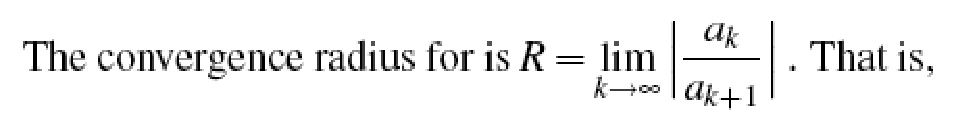
\includegraphics[width=0.55\textwidth]{latex}}}}
\subfigure{\label{word}}\addtocounter{subfigure}{-2}
\subfigure[Inline mode equation displayed as .doc format file derived from word software]{\subfigure[由~word软件生成的~.doc~格式行内公式]
          {\fbox{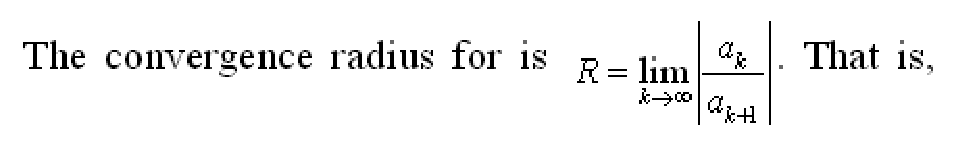
\includegraphics[width=0.55\textwidth]{word}}}}
\subfigure{\label{pdf}}\addtocounter{subfigure}{-2}
\subfigure[Inline mode equation displayed as .pdf format file derived from word software]{\subfigure[由~word软件生成的~.pdf~格式行内公式]
          {\fbox{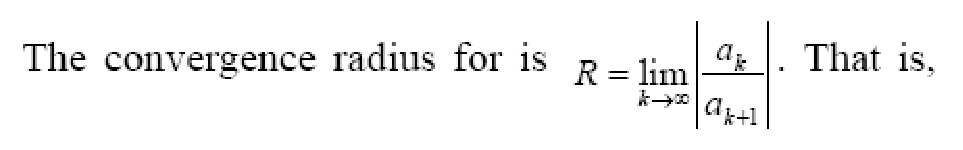
\includegraphics[width=0.55\textwidth]{pdf}}}}
\bicaption[hangju]{}{由~\LaTeX~和~word~生成的~3~种行内公式屏显效果}{Fig.$\!$}{Three kinds of inline mode equation displayed effects derived from \LaTeX and word}
\vspace{-1em}
\end{figure}
这三幅图分别为~\LaTeX~和~word~生成的行内公式屏显效果,从图中可看出,在~\LaTeX~文本含有公式的行内,在正文与公式之间对接工整,行距不变;而在~word~文本含有公式的行内,在正文与公式之间对接不齐,行距变大。因此从这一点来说,
\LaTeX~系统在数学公式的排版上具有很大优势。

\LaTeX~提供的行内公式最简单、最有效的方法是采用~\TeX~本来的标记———开始和结束标记都写作~\$,例如本节开始的例子可由下面的输入得到。
\verb|$f(x)=\int_{a}^{b}\frac{\sin{x}}{x}\mathrm{d}x$|

\BiSection{行间公式}{Displaymath mode equations}
位于两行之间的公式称为行间公式,每个公式都是一个单独的段落,例如
\[\int_a^b{f\left(x\right)\mathrm{d}x}=\lim_{\left\|\Delta{x_i}\right\|\to 0}\sum_i{f\left(\xi_i\right)\Delta{x_i}}\]
除人工编号外,\LaTeX~各种类型行间公式的标记见表~\ref{eqtag}。
\begin{table}[htbp]
\bicaption[eqtag]{}{各种类型行间公式的标记}{Table$\!$}{Tags for several kinds of displaymath mode equations}
\vspace{0.5em}\centering\wuhao
\begin{tabularx}{0.9\textwidth}{cXX}
\toprule
& 无编号 & 自动编号\\\midrule
单行公式 & \textbackslash begin\{displaymath\}...... \textbackslash end\{displaymath\}~或~\textbackslash [...\textbackslash ] & \textbackslash begin\{equation\} ...... \textbackslash end\{equation\}\\
多行公式 & \textbackslash begin\{eqnarray*\} ...... \textbackslash end\{eqnarray*\} & \textbackslash begin\{eqnarray\} ...... \textbackslash end\{eqnarray\}\\
\bottomrule
\end{tabularx}
\end{table}
另外,在自动编号的某行公式行尾添加标签~\verb|\nonumber|,可将该行转换为无编号形式。

行间多行公式需采用~\verb|eqnarray|~或~\verb|eqnarray*|~环境,它默认是一个列格式为~\verb|rcl|~的~3~列矩阵,并且中间列的字号要小一些,因此通常只将需要对齐的运算符号(通常为等号“=”)置于中间列。

\BiSection{可自动调整大小的定界符}{Delimiters with automatic adjustable sizes}
若在左右两个定界符之前分别添加命令~\verb|\left|~和~\verb|\right|,则定界符可根据所包围公式大小自动调整其尺寸,这可从式(\ref{nodelimiter})和式(\ref{delimiter})中看出。
\begin{equation}\label{nodelimiter}
(\sum_{k=\frac12}^{N^2})
\end{equation}
\begin{equation}\label{delimiter}
\left(\sum_{k=\frac12}^{N^2}\right)
\end{equation}
式(\ref{nodelimiter})和式(\ref{delimiter})是在~\LaTeX~中分别输入如下代码得到的。
\begin{lstlisting}
(\sum_{k=\frac12}^{N^2})
\left(\sum_{k=\frac12}^{N^2}\right)
\end{lstlisting}
\verb|\left|~和~\verb|\right|~总是成对出现的,若只需在公式一侧有可自动调整大小的定界符,则只要用“.”代替另一侧那个无需打印出来的定界符即可。

若想获得关于此部分内容的更多信息,可参见~\href{http://tug.ctan.org/cgi-bin/ctanPackageInformation.py?id=voss-mathmode}{Math mode}~文档的第~8~章“Brackets, braces and parentheses”。

\BiSection{数学重音符号}{Accents in math mode}
数学重音符号通常用来区分同一字母表示的不同变量,输入方法如下(需要调用~\verb|amsmath|~宏包):

\vspace{0.5em}\noindent\wuhao\begin{tabularx}{\textwidth}{Xc|Xc|Xc}
 \verb|\acute| & $\acute{a}$ & \verb|\mathring| & $\mathring{a}$ & \verb|\underbrace| & $\underbrace{a}$ \\
 \verb|\bar| & $\bar{a}$ & \verb|\overbrace| & $\overbrace{a}$ & \verb|\underleftarrow| & $\underleftarrow{a}$ \\
 \verb|\breve| & $\breve{a}$ & \verb|\overleftarrow| & $\overleftarrow{a}$ & \verb|\underleftrightarrow| & $\underleftrightarrow{a}$ \\
 \verb|\check| & $\check{a}$ & \verb|\overleftrightarrow| & $\overleftrightarrow{a}$ & \verb|\underline| & $\underline{a}$ \\
 \verb|\dddot| & $\dddot{a}$ & \verb|\overline| & $\overline{a}$ & \verb|\underrightarrow| & $\underrightarrow{a}$ \\
 \verb|\ddot| & $\ddot{a}$ & \verb|\overrightarrow| & $\overrightarrow{a}$ & \verb|\vec| & $\vec{a}$ \\
 \verb|\dot| & $\dot{a}$ & \verb|\tilde| & $\tilde{a}$ & \verb|\widehat| & $\widehat{a}$ \\
 \verb|\grave| & $\grave{a}$ & \verb|\underbar| & $\underbar{a}$ & \verb|\widetilde| & $\widetilde{a}$ \\
 \verb|\hat| & $\hat{a}$ 
\end{tabularx}\vspace{0.5em}
\xiaosi 当需要在字母~$i$~和~$j$~的上方添加重音符号时,为了去掉这两个字母顶上的小点,这两个字母应该分别改用~\verb|\imath|~和~\verb|\jmath|。

如果遇到某些符号不知道该采用什么命令能输出它时,则可通过~\href{http://detexify.kirelabs.org/classify.html}{Detexify$^2$~网站}来获取符号命令。若用鼠标左键在此网页的方框区域内画出你所要找的符号形状,则会在网页右方列出和你所画符号形状相近的~5~个符号及其相对应的~\LaTeX~输入命令。若所列出的符号中不包括你所要找的符号,还可通过点击“Select from the complete list!”的链接以得分从低到高的顺序列出所有符号及其相对应的~\LaTeX~输入命令。

最后,笔者建议大家还是要以~\href{http://tug.ctan.org/cgi-bin/ctanPackageInformation.py?id=voss-mathmode}{Math mode}~这篇~pdf~文档作为主要参考。若要获得最为标准、美观的数学公式排版形式,可以查查文档中是否有和你所要的排版形式相同或相近的代码段,通过修改代码段以获得你所要的数学公式排版形式。










% !Mode:: "TeX:UTF-8" 

\BiChapter{模板的其它说明}{Other explanation about the template}

\BiSection{中英文封面的相关信息}{Related information in Chinese and English covers}
国内图书分类号(Classif\/ied Index)的查询网址:

\centerline{\href{http://www.ztflh.com/}{http://www.ztflh.com/}——中国图书馆分类法}
国际图书分类法(U.D.C)的查询网址:

\centerline{\href{http://www.udcc.org/udcsummary/php/index.php}{http://www.udcc.org/udcsummary/php/index.php}——UDC Summary}
学校代码查询网址:

\centerline{\href{http://www.marry360.com.cn/Tools/UniversityCodeList.aspx}{http://www.marry360.com.cn/Tools/UniversityCodeList.aspx}——高校代码查询}
\noindent 哈尔滨工业大学的学校代码为~10213。

英文封面下方的学位论文相关信息可以采用~\verb|tabular|~和~\verb|tabularx|~两种表格环境,具体使用哪一种环境和具体的相关信息有关。若信息内容不太长,不会引起信息内容分行时,则应该采用~\verb|tabular|~环境;若信息内容过长,会引起信息内容分行时,则应该采用~\verb|tabularx|~环境。具体用法请见~format.tex~文件的相应代码。

\BiSection{\textsc{Bib}\kern-.08em\TeX~文献文件的写法}{How to write the \textsc{Bib}\kern-.08em\TeX~bibliographic file}
用在~\LaTeX~中的~\textsc{Bib}\kern-.08em\TeX~文献文件的扩展名为~bib,此模板中,该文件即为~reference.bib。bibtex.exe 命令根据~GBT7714-2005NLang-HIT.bst 文件定义的文献格式,将~reference.bib 中的文献数据转换为输出文档中的文献列表。GBT7714-2005NLang-HIT.bst 文件是在~\href{http://bbs.ctex.org/attachment.php?aid=MjA3MDh8ZDcyMjc2MTN8MTMyNTYzNjY4OHxhZTg4bkNCUVJiRzA0WmU3TmlMbVdTUVExa0xtV2puWWc0dkdqbVJhbTVMdy9mVQ\%3D\%3D}{GBT7714-2005NLang-UTF8.bst} 文件的基础上修改得到的,所做的唯一一处改动是将姓氏字母全部大写的英文作者名改为只首字母大写,以保证和\href{http://219.217.226.141/xuewei/guifan.doc}{《研究生学位论文撰写规范》}及其\href{http://219.217.226.141/xuewei/fanli.doc}{《研究生学位论文书写范例》}相一致。

bib 文件的编写方法可参考模板中已给出的例子,也可参考~\href{http://bbs.ctex.org/attachment.php?aid=MTk3OTd8NjY1ODc5OGV8MTMyNTY0MTEyMnxhZGZkYWpsa0I2RGZwNDR5Z1lyeStjb1dKRS8rTnJub3lvT2FkNDNJbHl1UWVkVQ\%3D\%3D}{GBT7714-2005.bst说明文档20060919
} 中所给出的例子。

中文文献需要添加一个额外的~language 域,并使得域值非空,这样~bst 文件就能够判断此文献为中文文献,进而能正确地生成参考文献格式。

GBT7714-2005.bst 对于国标~GB/T 7714-2005 的文献分类如表~\ref{tab:entrytypes} 所示。对于每种文献类型的缺省类型,已经设置好相应的文献标识码,因此不需要输入相应的文献
标识码。扩展类型的文献则应再添加一个~TypeofLit 域,并需要将其域值改为相应的文献标识码。
\begin{table}[htbp]
\bicaption[tab:entrytypes]{}{GBT7714-2005.bst 的分类方式}{Table$\!$}{Classification method of GBT7714-2005.bst}
\vspace{0.5em}\centering\wuhao
\begin{tabular}{llll}
\toprule[1.5pt]
文献类型 & 缺省类型 & 扩展类型(需要手 & 主要特征\\
 &  & 工加入文献标识码) & \\
\midrule[1pt]
article & 文章[J] & 报纸中的析出文献[N] & 年,卷(期):页码\\
 &  & 在线文章[J/OL] & \\
book & 书[M] & 论文集、会议录[C] & \\
 &  & 在线书[M/OL] & \\
 &  & 汇编[G] & \\
inbook & 书的某几页[M] &  & \\
incollection & 书中析出的文章[M]// & 汇编的析出文献[G]// & 析出文献[文献标识码]//\\
 &  & 标准的析出文献[S]// & \\
proceedings &  &  & \\
inproceedings & 论文集、会议录中的 & 在线论文集、 & 析出文献[文献标识码]//\\
/conference & 析出文献[C]// & 会议录[C/OL]// & \\
mastersthesis & 毕业论文[D] &  & 类似book类\\
phdthesis & 毕业论文[D] &  & 类似book类\\
techreport & 科技报告[R] &  & 类似book类\\
misc &  & 杂项[],例如:专利[P] & 此类一般是网上文件,\\
 &  & 网上专利[P/OL] & 按照国标规定顺序\\
 &  & 网上电子公告[EB/OL] & 编码制时不输出年份\\
 &  & 磁盘[CP/DK] & \\
\bottomrule[1.5pt]
\end{tabular}
\end{table}

《研究生学位论文撰写规范》及《研究生学位论文书写范例》中所列英文参考文献例子中的文章名的每个实词首字母都大写,因此需要将英文参考文献的~title 域手动修改为每个实词首字母大写。

英文参考文献在~author 域中的作者名需要将姓置前,名置后。

\BiSection{参考文献的引用}{Citation of references}
需要将~main.tex 文件中的语句~\verb|\nocite{*}| 屏蔽掉,这样,文中未引用的参考文献就不会出现在文后的参考文献列表中。文中参考文献的引用方法:

\begin{itemize}
\item 行文引用请使用命令~\verb|\cite{引用词}|,引用效果为“\cite{lin1992}”;
\item 上标引用请使用命令~\verb|\citeup{引用词}|,引用效果为“\citeup{lin1992}”。
\end{itemize}
其中,上标引用命令~\verb|\citeup{}| 为本模板自定义的命令,其定义为
\begin{verbatim}
\newcommand{\citeup}[1]{\textsuperscript{\cite{#1}}}
\end{verbatim}

\BiSection{单层罗列环境}{Monolayer list environment}
哈工大学位论文一般可采用两种罗列环境:一种是并列条目有同样标签的~\verb|itemize|~罗列环境,另一种是具有自动排序编号符号的~\verb|enumerate|~罗列环境。这两种罗列环境的样式参数可参考图~\ref{list}。
\begin{figure}[htbp]
\centering
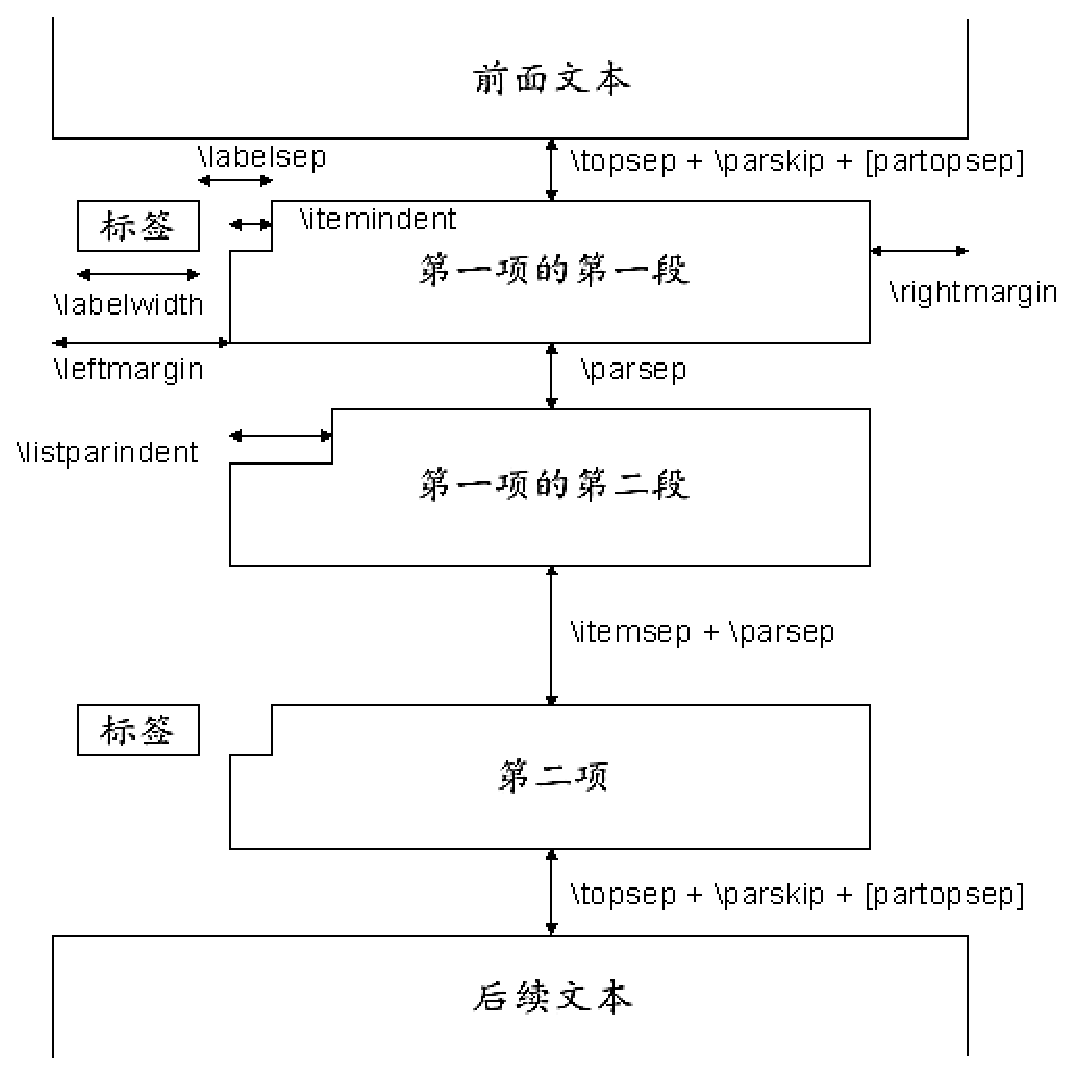
\includegraphics[width = 0.6\textwidth]{list}
\bicaption[list]{}{罗列环境参数示意图}{Fig.$\!$}{Schematic diagram of list environments}\vspace{-1em}
\end{figure}
通过调用~enumitem~宏包可以很方便地控制罗列环境的布局,其~format.tex~文件中的~\verb|\setitemize|~和~\verb|\setenumerate|~命令分别用来设置~\verb|itemize|~和~\verb|enumerate|~环境的样式参数。采用~\verb|itemize|~单层罗列环境的排版形式如下:
\begin{itemize}
\item 第一个条目文本内容
\item 第二个条目文本内容
\item 第三个条目文本内容
\end{itemize}
其代码如下
\begin{verbatim}
\begin{itemize}
  \item 第一个条目文本内容
  \item 第二个条目文本内容
  ...
  \item 第三个条目文本内容
\end{itemize}
\end{verbatim}
采用~\verb|enumerate|~单层罗列环境的排版形式如下:
\begin{enumerate}
\item 第一个条目文本内容
\item 第二个条目文本内容
\item 第三个条目文本内容
\end{enumerate}
其代码如下
\begin{verbatim}
\begin{enumerate}
  \item 第一个条目文本内容
  \item 第二个条目文本内容
  ...
  \item 第三个条目文本内容
\end{enumerate}
\end{verbatim}

\BiSection{算法}{Algorithm}

这是一个算法的例子,来自~worldguy@lilacbbs。建议将算法放在~minipage~环境中,避免算法出现在页面版心之外。

\begin{algorithm}
\KwIn{training samples, {$(d_i, d_j)_q$; $\mathbf{q}_i, \mathbf{q}_j \in C$,
$q\in \mathbf{Q}$} }
\KwOut{parameter setting $\lambda^T$}%

\For{$t$=1 to $T$}
{   
    $\lambda^{t+1}_n = \lambda^t_n + \eta (f_n(q, c, d_i) - f_n(q, c, d_j))$
 }
\end{algorithm}

%\KwIn{training samples, {$(d_i, d_j)_q$; $\mathbf{q}_i, \mathbf{q}_j \in C$,
%$q\in \mathbf{Q}$} }
%\KwOut{parameter setting $\lambda^T$}%
%
%\For{$t$=1 to $T$}
%{   
%    $\lambda^{t+1}_n = \lambda^t_n + \eta (f_n(q, c, d_i) - f_n(q, c, d_j))$
% }
%\end{algorithm}

算法环境中右侧空白比较多,若想把右侧的空白框减小,可以采用~minipage~环境实现。把~algorithm~环境放到~minipage~环境里面,并且加上选项[H]禁止算法浮动,下面给出一个例子。需要说明的是,一般不需要进行这种处理。算法标题可有可无,若有中英文标题,请使用~\verb|\AlgoBiCaption{中文标题}{英文标题}|。下面给出两个有标题的例子。需要说明的是,算法的标题是自动换行,没有必要手动换行。

\begin{minipage}{0.8\textwidth}\centering
\begin{algorithm}[H]
 \AlgoBiCaption{这是一个简短的算法中文图题}{This is the English caption of the algorithm}
  \KwIn{training samples, {$(d_i, d_j)_q$; $\mathbf{q}_i, \mathbf{q}_j
      \in C$, $q\in \mathbf{Q}$} }
 \KwOut{parameter setting
    $\lambda^T$}
 \For{$t$=1 to $T$} { $\lambda^{t+1}_n = \lambda^t_n +
    \eta (f_n(q, c, d_i) - f_n(q, c, d_j))$ }
\end{algorithm}
\end{minipage}


\begin{minipage}{0.9\textwidth}\centering
\begin{algorithm}[H]
 \AlgoBiCaption{这是一个算法的比较长的中文图题,需要换行,这里采用自动换行,如果手动换行会造成算法目录中同样出现断行}{This is a long English caption of the algorithm, a new line  required, and this a new line}
  \KwIn{training samples, {$(d_i, d_j)_q$; $\mathbf{q}_i, \mathbf{q}_j
      \in C$, $q\in \mathbf{Q}$} }
 \KwOut{parameter setting
    $\lambda^T$}
 \For{$t$=1 to $T$} { $\lambda^{t+1}_n = \lambda^t_n +
    \eta (f_n(q, c, d_i) - f_n(q, c, d_j))$ }
\end{algorithm}
\end{minipage}

\BiSection{定理定义}{Theorem and definition}

若需要书写定理定义等内容,而且带有顺序编号,需要采用如下环境。除了~\verb|proof|~环境之外,其余~9~个环境都可以有一个可选参数作为附加标题。

\begin{center}\vspace{0.5em}\noindent\wuhao\begin{tabularx}{0.7\textwidth}{lX|lX}
定理 & \verb|theorem|~环境 & 定义 & \verb|definition|~环境 \\
例 & \verb|example|~环境 & 算法 & \verb|algo|~环境 \\
公理 & \verb|axiom|~环境 & 命题 & \verb|proposition|~环境 \\
引理 & \verb|lemma|~环境 & 推论 & \verb|corollary|~环境 \\
注解 & \verb|remark|~环境 & 证明 & \verb|proof|~环境 \\
\end{tabularx}\end{center}
% !Mode:: "TeX:UTF-8" 

\BiAppendixChapter{结\quad 论}{Conclusions}

%学位论文的结论作为论文正文的最后一章单独排写,但不加章标题序号。

%结论应是作者在学位论文研究过程中所取得的创新性成果的概要总结,不能与摘要混为一谈。博士学位论文结论应包括论文的主要结果、创新点、展望三部分,在结论中应概括论文的核心观点,明确、客观地指出本研究内容的创新性成果(含新见解、新观点、方法创新、技术创新、理论创新),并指出今后进一步在本研究方向进行研究工作的展望与设想。对所取得的创新性成果应注意从定性和定量两方面给出科学、准确的评价,分(1)、(2)、(3)…条列出,宜用“提出了”、“建立了”等词叙述。

软件中克隆代码随着系统演化,克隆代码的存在以及在演化过程中会发生变化,导致软件难以理解和维护,已经成为了影响软件质量的一个重要因素。现有的研究方法中既不能客观全面的理解克隆代码,也不能有效地解决克隆代码一致性变化问题。针对以上问题,本文提出了基于软件演化的克隆代码分析与一致性维护方法,重点研究了克隆代码演化特征分析、克隆代码创建时和变化时的一致性需求预测和跨项目的克隆代码一致性预测,取得了如下创新性成果:

(1) 针对现有的克隆分析方法不能全面客观地理解克隆代码及其演化过程,提出了一个基于聚类的克隆代码演化特征分析方法。方法通过检测软件版本中的克隆代码,并构建系统克隆家系描述克隆代码的演化过程。为表示克隆代码及其演化情况,从克隆片段、克隆组和克隆家系三个不同的角度提取相应的属性值。在此基础上使用X-means聚类分析和挖掘克隆代码的演化特征。实验表明软件中存在的大部分克隆代码在其演化过程中是较为稳定的,并不会发生频繁的变化。同时,也存在一定规模的发生变化的克隆代码,其中发生一致性变化的克隆要多于不一致变化的克隆代码。

(2)针对新创建的克隆代码在其演化过程可能会引发一致性变化,从而导致额外的维护代价问题,提出了克隆代码创建时一致性维护需求预测方法。提供了一个克隆代码创建时的一致性维护需求定义,将问题转化为一个可以使用机器学习解决的分类问题。通过构建系统克隆家系并识别克隆演化模式,从系统中收集克隆创建实例用于训练机器学习模型,并提取代码属性和上下文属性表示创建的克隆代码。在四个实验系统上使用五种不同机器学习方法进行了评估,实验表明该方法以较高的准确率和召回率高效地预测克隆代码创建时的一致性维护需求。

(3)针对演化过程中的克隆代码的一致性变化可能引发的一致性缺陷问题,提出了克隆代码变化时一致性维护需求预测方法。提供了克隆代码变化时的一致性维护需求定义,将问题装化为可以应用机器学习方法解决的分类问题。通过构建系统的克隆家系和识别其演化模式,从系统中收集克隆变化实例用于训练机器学习模型。从克隆组的角度提取了代码属性、上下文属性,并同时从克隆演化的角度提取了一组演化属性共同表示克隆变化实例。在四个实验系统上使用五种不同机器学习方法进行了评估,实验表明该方法以合理的准确率和召回率有效地预测克隆代码变化使得一致性维护需求。

(4)针对软件开发初期系统缺少训练数据的情况,提出了跨项目的克隆代码一致性维护需求预测方法。统一克隆创建和变化时的一致性维护需求,为克隆一致性维护需求定义。使用训练系统训练机器学习模型,并在测试系统上进行跨项目一致性预测。同时,还结合软件开发过程,基于eclipse设计并实现了一个克隆代码一致性维护需求预测插件,可以在实际开发中帮助程序开发人员预测克隆代码的一致性维护需求。在四个实验系统上使用五种不同机器学习方法进行了实证研究,结果表明跨项目预测可以在软件开发初期进行克隆一致性预测,并给出了一些建议帮助提高跨项目的预测能力。该方法可以在软件开发过程中帮助程序开发人员边开发、边预测克隆代码的一致性维护需求。

在本文工作的基础上,还有以下工作有待于进一步研究:

(1) 在克隆变化时一致性维护需求预测中,仍然有一定的改进空间。在未来研究中,拟通过改进现有的属性表示克隆代码的真实变化,从而以更高的准确率和召回率高效的预测克隆代码的一致性维护需求。

(2)在预测跨项目的克隆一致性维护需求时,方法的预测能力尚未达到令人满意的效果。在未来的研究中,拟通过添加与项目自身相关的属性、选择更为合适的实例提高跨项目的预测能力,从而帮助缺乏训练数据的新系统进行一致性维护需求预测。

(3)在软件开发过程中,本文方法仅可以警告程序开发人员克隆代码的一致性维护需求,并没有对克隆代码进行一致性维护。在未来的研究中,拟结合程序分析技术,在需要时对克隆代码自动地进行一致性维护,从而保证克隆代码的一致性。同时,结合克隆一致性预测方法,帮助识别并修复系统中已存在的一致性缺陷,从而提高软件质量。   % 结论

%\BiChapter{图片的插入方法}{Methods of inserting figures}

\BiSection{单张图片的插入方法}{The method of inserting one single figure}

\BiSubsection{条标题}{The caption of subsection}

单张图片独自占一行的插入形式如图~\ref{golfer1}~所示。
\begin{figure}[htbp]
\centering
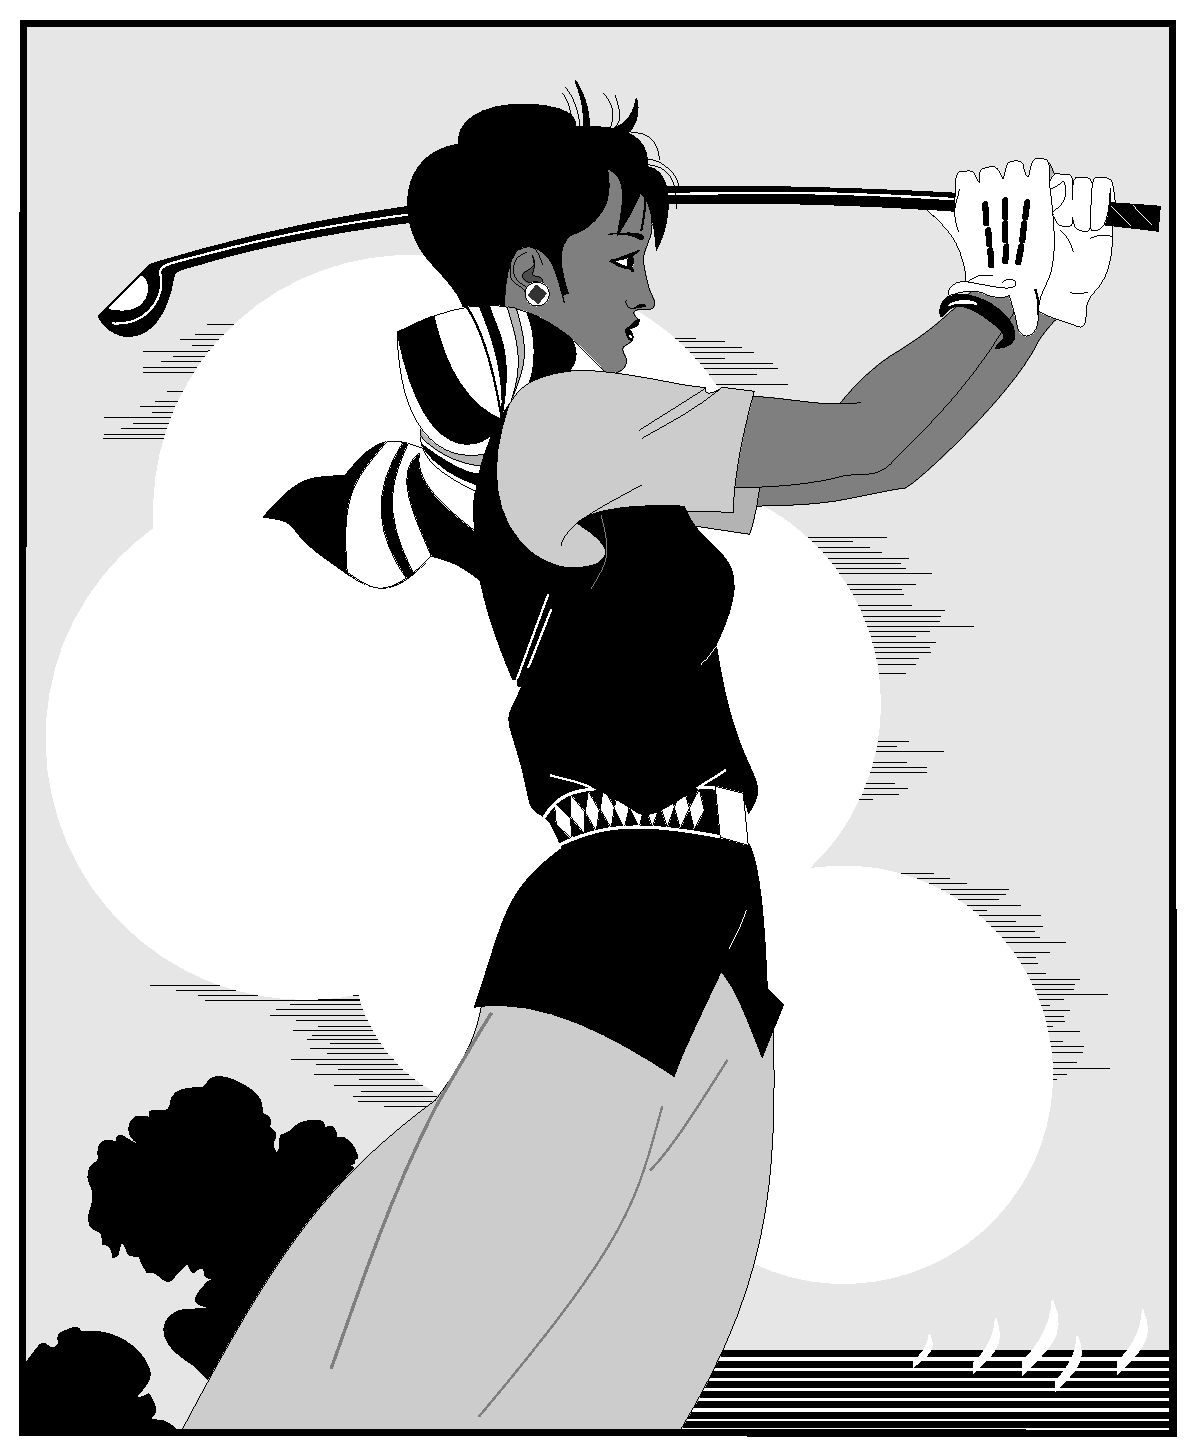
\includegraphics[width = 0.4\textwidth]{golfer}
\bicaption[golfer1]{}{打高尔夫球的人}{Fig.$\!$}{The person playing golf}\vspace{-1em}
\end{figure}

其插入图片的代码及其说明如下。
\begin{verbatim}
\begin{figure}[htbp]
\centering
\includegraphics[width=0.4\textwidth]{文件名(.eps)}
\bicaption[标签名(英文)]{}{中文标题}{Fig.$\!$}
          {English caption (首字母大写)}\vspace{-1em}
\end{figure}
\end{verbatim}
%\BiChapter{表格的绘制方法}{Methods of drawing tables}

\BiSection{普通表格的绘制方法}{Methods of drawing normal tables}


表格应具有三线表格式,因此需要调用~booktabs~宏包,其标准格式如表~\ref{table1}~所示。
\begin{table}[htbp]
\bicaption[table1]{}{符合研究生院绘图规范的表格}{Table$\!$}{Table in agreement of the standard from graduate school}
\vspace{0.5em}\centering\wuhao
\begin{tabular}{ccccc}
\toprule[1.5pt]
$D$(in) & $P_u$(lbs) & $u_u$(in) & $\beta$ & $G_f$(psi.in)\\
\midrule[1pt]
 5 & 269.8 & 0.000674 & 1.79 & 0.04089\\
10 & 421.0 & 0.001035 & 3.59 & 0.04089\\
20 & 640.2 & 0.001565 & 7.18 & 0.04089\\
\bottomrule[1.5pt]
\end{tabular}
\end{table}

其绘制表格的代码及其说明如下。
\begin{verbatim}
\begin{table}[htbp]
\bicaption[标签名]{}{中文标题}{Table$\!$}{English caption}
\vspace{0.5em}\centering\wuhao
\begin{tabular}{cc...c}
\toprule[1.5pt]
表头第1个格   & 表头第2个格   & ... & 表头第n个格  \\
\midrule[1pt]
表中数据(1,1) & 表中数据(1,2) & ... & 表中数据(1,n)\\
表中数据(2,1) & 表中数据(2,2) & ... & 表中数据(2,n)\\
...................................................\\
表中数据(m,1) & 表中数据(m,2) & ... & 表中数据(m,n)\\
\bottomrule[1.5pt]
\end{tabular}
\end{table}
\end{verbatim}
%\BiChapter{数学公式的输入方法}{Input methods of equations}

\BiSection{行内公式}{Inline mode equations}

出现在正文一行之内的公式称为行内公式,例如~$f(x)=\int_{a}^{b}\frac{\sin{x}}{x}\mathrm{d}x$。对于非矩阵和非多行形式的行内公式,一般不会使得行距发生变化。

\BiSection{行间公式}{Displaymath mode equations}

位于两行之间的公式称为行间公式,每个公式都是一个单独的段落,下边的例子是一个无编号的行间单行公式

\[
\int_a^b{f\left(x\right)\mathrm{d}x}=\lim_{\left\|\Delta{x_i}\right\|\to 0}\sum_i{f\left(\xi_i\right)\Delta{x_i}}
\]

下边的例子是一个无编号的行间多行公式(\ref{lizi})
\begin{eqnarray*}\label{lizi}
\sin 2x&=&2\sin x\cos x\\
\cos 2x&=&2\cos x^2-1=1-2\sin x^2=\cos x^2-\sin x^2
\end{eqnarray*}
%参考文献\cite{OOSTRUM01}和参考文献\citeup{wwwlixing}


%参考文献
\defaultfont
\bibliographystyle{GBT7714-2005NLang-HIT}
\addcontentsline{toc}{chapter}{参考文献}      % 参考文献加入到中文目录
\addcontentsline{toe}{chapter}{\bfseries  References} % 参考文献加入到英文目录
\addtolength{\bibsep}{-0.8em}
%\nocite{*}  %若将此命令屏蔽掉,则未引用的文献不会出现在文后的参考文献列表中。
\bibliography{reference}
% -*-coding: utf-8 -*-

\defaultfont
\appendix

%%%%%%%%%%%%%%%%%%%%%%%%%%%%%%%%%%%%%%%%%%%%%%%%%%%%%%%%%
\BiAppChapter{带章节的附录}{Full Appendix}%
完整的附录内容,包含章节,公式,图表等

%%%%%%%%%%%%%%%%%%%%%%%%%%%%%%%%%%%%%%%%%%%%%%%%%%%%%%%%%
\BiSection{附录节的内容}{Section in Appendix}
这是附录的节的内容

附录中图的示例:
\begin{figure}[htbp]
\centering
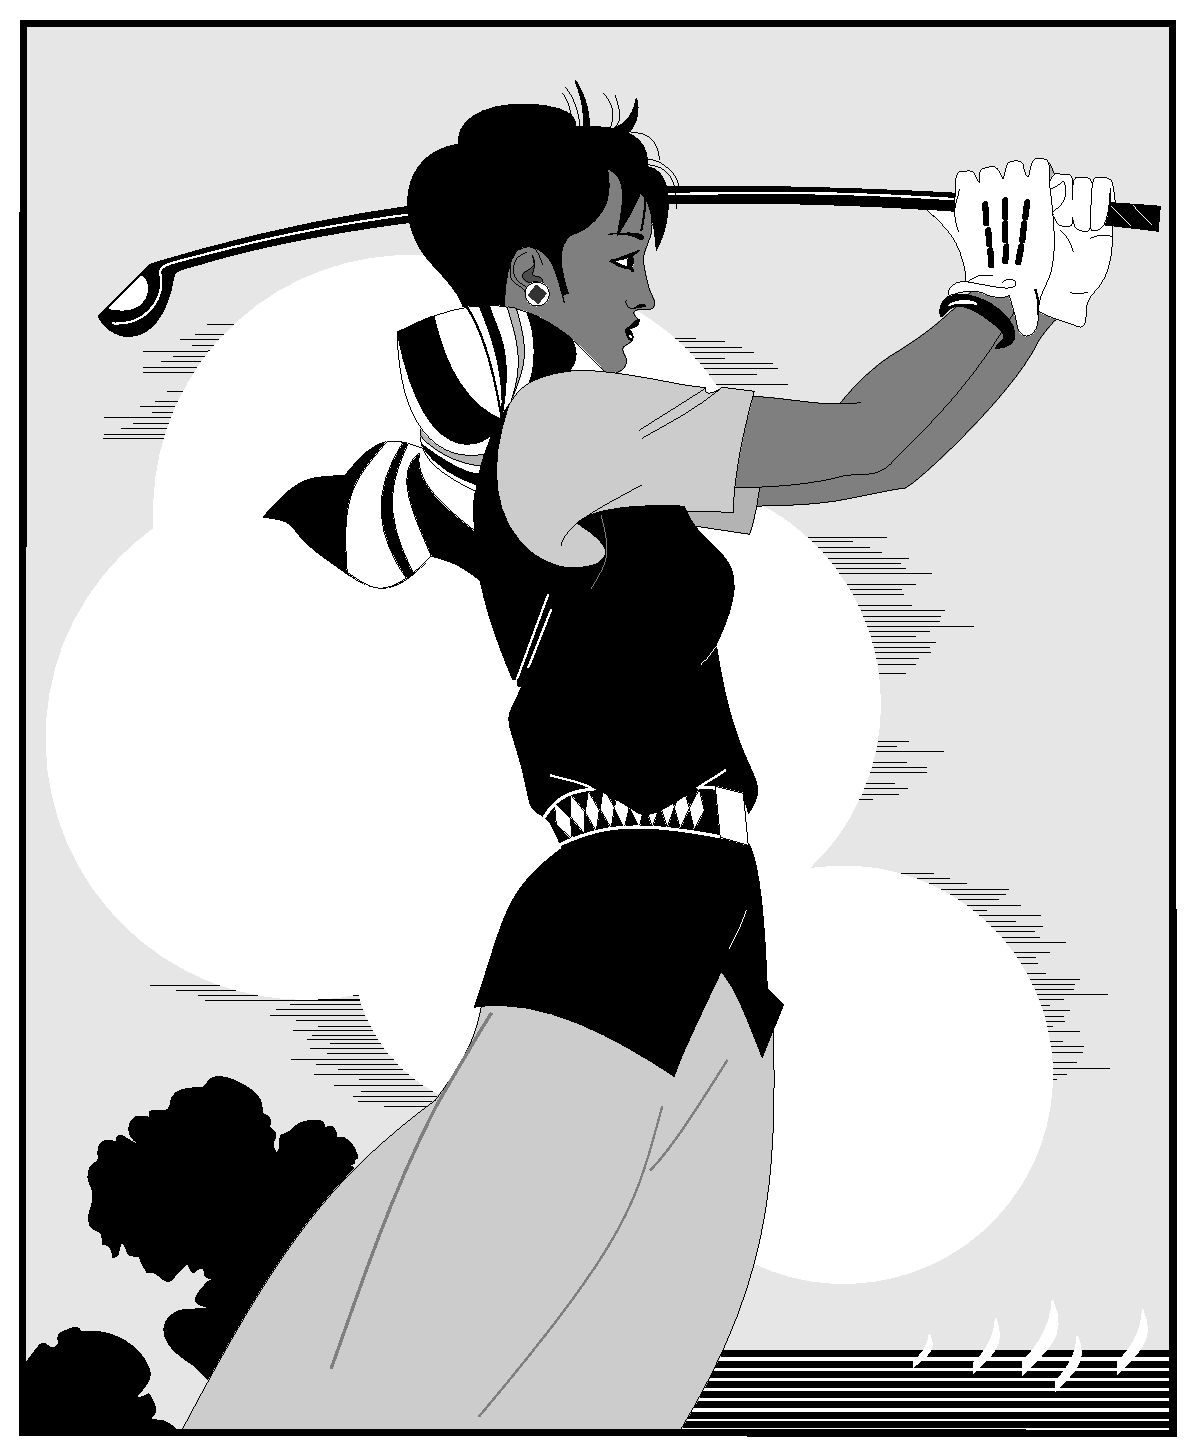
\includegraphics[width = 0.4\textwidth]{golfer}
\bicaption[golfer5]{}{打高尔夫球的人}{Fig.$\!$}{The person playing golf}\vspace{-1em}
\end{figure}

附录中公式的示例:
\begin{align}
a & = b \times c \\
E & = m c^2
\end{align}

\BiAppChapter{这个星球上最好的免费Windows软件列表}{List of the Best Free Windows Software in our Planet}
\section*{杀毒软件}
\href{http://www.avast.com/zh-cn/free-antivirus-download}{avast! 免费杀毒软件}——推荐

\href{http://www.avg.com/cn-zh/china-avg-antivirus-free}{AVG 杀毒永久免费版}——推荐

\href{http://www.avira.com/en/avira-free-antivirus}{Avira Free Antivirus (小红伞)}









%\BiAppChapter{附录三}{appendix 3}    % 附录
% !Mode:: "TeX:UTF-8" 

\BiAppendixChapter{攻读\cxuewei 学位期间发表的论文及其他成果} {Papers
published in the period of PH.D. education}
\noindent\textbf{(一)已发表的学术论文}
%\noindent\textbf{(一)已发表的(含录用)学术论文}
\begin{publist}

\item
\underline{Zhang Fanlong}, Khoo Siau-Cheng, Su Xiaohong{$^*$}. Predicting Change Consistency in A Clone Group[J]. Journal of Systems and Software. 134(2017), 105-119.
(已发表, DOI:10.1016/j.jss.2017.08.045, SCI收录,  5-Year IF=2.619, CCF推荐B类期刊, 中科院SCI期刊分区3区, 对应第4章, 第一作者)
%2016年IF=2.444, 

\item
\underline{Zhang Fanlong}, Khoo Siau-Cheng, Su Xiaohong{$^*$}. Predicting Consistent Clone Change[C]. Proceeding of the 27th International Symposium on Software Reliability Engineering (ISSRE), Ottawa, Canada, 2016: 353-364.
(已发表, DOI:10.1109/ISSRE.2016.11, EI:20170803379101, CCF推荐B类会议, 对应第4章, 第一作者)

\item
\underline{Zhang Fanlong}, Khoo Siau-cheng, Su Xiaohong{$^*$}. Machine-Learning Aided Analysis of Clone Evolution[J/OL]. Chinese Journal of Electronics(2017-09-28). http://kns.cnki.net/kcms/detail/10.1284.TN.20170928.1353.002.html.
(已发表, DOI:10.1049/cje.2017.08.012, SCI收录, 2016年IF=0.513, 中科院分区4区, 对应第2章, 第一作者)

%%%\item
%%%\underline{Zhang Fanlong}, Khoo Siau-cheng, Su Xiaohong{$^*$}. Machine-Learning Aided Analysis of Clone Evolution[J]. Chinese Journal of Electronics.  26(2017).
%%%(已发表, DOI:10.1049/cje.2017.08.012, SCI收录, 2016年IF=0.513, 中科院分区4区, 对应第2章, 第一作者)

\item
苏小红, \underline{张凡龙}{$^*$}. 面向管理的克隆代码研究综述[J/OL]. 计算机学报2017(2017-08-24). On Publishing: No.120, Vol.40. http://kns.cnki.net/kcms/detail/11.1826.TP.20170728.1305.046.html.
(已发表, EI收录, 一级学报, 对应第1章, 第二作者, 导师为第一作者)

%%%\item
%%%苏小红, \underline{张凡龙}{$^*$}. 面向管理的克隆代码研究综述[J/OL]. 计算机学报2017(2017-07-28) [2017-08-24]. http://kns.cnki.net/kcms/detail/11.1826.TP.20170728.1305.046.html.
%%%(网络优先发表, EI收录, 一级学报, 对应第1章, 第二作者, 导师为第一作者)

\item
\underline{Zhang Fanlong }, Su Xiaohong{$^*$},  Zhao Wen,  Ma Peijun. An Empirical Study of Code Clone Clustering Based on Clone Evolution[J]. Journal of Harbin Institute of Technology(New Series).2017, 24(2):10-18.
(已发表, DOI:10.11916/j.issn.1005-9113.15316, 哈工大学报英文版, 对应第2章, 第一作者)

\item
\underline{张凡龙}, 苏小红{$^*$},  李智超,  马培军. 基于支持向量机的克隆代码有害性评价方法[J]. 智能计算机与应用, 2016, 6(4): 112-115. 
(已发表, 对应第3章, 第一作者)

\item
Su Xiaohong{$^*$}, \underline{Zhang Fanlong},  Xia Li, et al. Functionally Equivalent C Code Clone Refactoring by Combining Static Analysis with Dynamic Testing[C]. Proceeding of the International Conference on Soft Computing Techniques and Engineering Application. 2014: 247-256.
(已发表, DOI: 10.1007/978-81-322-1695-7\_28, EI:20151600752325, 第二作者, 导师为第一作者)
\end{publist}

\noindent\textbf{(二)审稿中的学术论文}
\begin{publist}

\item
\underline{Zhang Fanlong},  Khoo Siau-Cheng, Su Xiaohong{$^*$}. An Empirical Study on Clone Consistency-Requirement Prediction Based on Machine Learning[J]. Journal of Computer Science and Technology.
(大修, SCI收录, 2016年IF=0.956, CCF推荐B类期刊, 中科院SCI期刊分区4区, 对应第5章, 第一作者)

\item
\underline{Zhang Fanlong}, Khoo Siau-cheng, Su Xiaohong{$^*$}. Improving Maintenance-Consistency Prediction During Code Clone Creation[J]. Software Quality Journal. 
(在审, SCI收录, 2916年IF=1.816, CCF推荐C类期刊, 中科院SCI期刊分区4区, 对应第3章, 第一作者)

\item
\underline{Zhang Fanlong }, Su Xiaohong{$^*$}. Cross-Project Clone Consistency Prediction[J]. Journal of Systems and Software.
(在审, SCI收录, 5-Year IF=2.619, 2016年IF=2.444, CCF推荐B类期刊, 中科院SCI期刊分区3区, 对应第5章, 第一作者)
%Cluster Computing. (在审, SCI收录, 2016年IF=2.040, 中科院SCI期刊分区3区, 对应第5章, 第一作者)

%\item 放弃
%\underline{Zhang Fanlong }, Su Xiaohong.  CCP: An Plug-in for Clone Consistency Prediction[C] 
%(在投, 对应第5章, 第一作者)

%\item 放弃
%\underline{张凡龙 }, 何蔷, 苏小红{$^*$}. 克隆代码可视化方法研究[J].哈尔滨工业大学学报.
% (在投, EI收录, 第一作者)

\end{publist}

\noindent\textbf{(三)与他人合作的学术论文}
\begin{publist}
\item
Yuan Yue, \underline{Zhang Fanlong},  Su Xiaohong{$^*$}. CloneAyz: An Approach for Clone Representation and Analysis[C]. Proceeding of the 3rd International Conference on Information Science and Control Engineering (ICISCE), 2016: 252-256.(已发表, EI:20165003106894, DOI:10.1109/ICISCE.2016.63, 第二作者)
\end{publist}

%%\noindent\textbf{(二)申请及已获得的专利(无专利时此项不必列出)}
%%\begin{publist}
%%\item XXX,XXX. 一种温热外敷药制备方案:中国,88105607.3[P]. 1989-07-26.
%%\end{publist}
\noindent\textbf{(四)参与的科研项目}
\begin{publist}

\item
苏小红等. 建筑全性能联合仿真平台内核开发. “十三五”国家重点研发计划课题. 课题编号:2017YFC0702204.
\item	
苏小红等. 基于启发式选择变异和软件行为特征挖掘的软件错误定位方法. 国家自然科学基金项目. 课题编号:61672191.
\item	
苏小红等. 无定型克隆代码的检测及重构方法. 国家自然科学基金项目. 课题编号:61173021.
\item
苏小红等. 数据挖掘和静态分析相结合的克隆代码缺陷检测及重构方法. 国家自然科学基金项目. 课题编号:61073052.
\item
苏小红等. 面向理解的软件错误定位方法. 国家自然科学基金项目. 课题编号:61202092.

\item
苏小红等. 基于程序转换和语义分析的编程自动评分方法研究. 国家自然科学基金项目. 课题编号:60673035.

\end{publist}
\vfill
\hangafter=1\hangindent=2em\noindent

\setlength{\parindent}{2em}
    % 所发文章
% !Mode:: "TeX:UTF-8" 

\BiAppendixChapter{哈尔滨工业大学学位论文原创性声明和使用权限}{Statement of copyright and Letter of authorization}
\vspace{\baselineskip}
\begin{center}\hei\xiaosan{学位论文原创性声明}\end{center}
\vspace{1em}

本人郑重声明:此处所提交的学位论文《\chinesethesistitle》,是本人在导师指导下,在哈尔滨工业大学攻读学位期间独立进行研究工作所取得的成果,且学位论文中除已标注引用文献的部分外不包含他人完成或已发表的研究成果。对本学位论文的研究工作做出重要贡献的个人和集体,均已在文中以明确方式注明。

\vspace{\baselineskip}
\hspace{6em}作者签名:\hfill 日期:\hspace{2.5em}年\hspace{1.5em}月\hspace{1.5em}日

\vspace{2\baselineskip}
\begin{center}\hei\xiaosan{学位论文使用权限}\end{center}
\vspace{1em}

学位论文是研究生在哈尔滨工业大学攻读学位期间完成的成果,知识产权归属哈尔滨工业大学。学位论文的使用权限如下:

(1)学校可以采用影印、缩印或其他复制手段保存研究生上交的学位论文,并向国家图书馆报送学位论文;(2)学校可以将学位论文部分或全部内容编入有关数据库进行检索和提供相应阅览服务;(3)研究生毕业后发表与此学位论文研究成果相关的学术论文和其他成果时,应征得导师同意,且第一署名单位为哈尔滨工业大学。

保密论文在保密期内遵守有关保密规定,解密后适用于此使用权限规定。

本人知悉学位论文的使用权限,并将遵守有关规定。


\vspace{2\baselineskip}
\hspace{6em}作者签名:\hfill 日期:\hspace{2.5em}年\hspace{1.5em}月\hspace{1.5em}日

\vspace{2\baselineskip}
\hspace{6em}导师签名:\hfill 日期:\hspace{2.5em}年\hspace{1.5em}月\hspace{1.5em}日   % 承诺
% !Mode:: "TeX:UTF-8" 

\BiAppendixChapter{致\quad 谢}{Acknowledgements}

在此论文完成之际,谨向给予我无私帮助和关怀的人们致以最诚挚的谢意!

衷心感谢我的导师苏小红教授!本文是在苏老师的悉心指导下完成的,几年来苏老师对我的科研工作给予了大力支持,也在日常生活等等方面给予了无微不至的关怀。在攻读博士期间,论文的选题、开题、中期以及博士论文撰写的各个阶段,苏老师给予了细致且精心的指导,在此向她表达最衷心的感谢,她的言传身教将使我终生受益。苏老师渊博的知识、远见的学术洞察力、严谨的治学态度和执着的敬业精神使我受益匪浅。没有苏老师的悉心指导和热情鼓励,我的博士论文工作不可能如此顺利的完成。在此,谨向恩师致以由衷的敬意和衷心的感谢!

衷心感谢新加坡国立大学的Khoo Siau-Cheng教授!在新加坡国立大学访学期间,Prof. Khoo悉心地指导我进行学术研究,细致地与我讨论学术问题,认真的帮我修改学术论文。Prof. Khoo严谨的治学态度、卓越的学术能力将是我终生学习的方向!

衷心感谢所有对本文提出宝贵意见的专家们,尤其是责任专家、外审专家以及答辩专家!在所有专家的帮助、批评和指正下,使得本文更加完善。

衷心感谢实验室全体老师和同窗们的热情帮助和支持!感谢王甜甜老师、张彦航老师、赵玲玲老师!感谢实验室的师兄师姐师弟师妹们!

衷心感谢我的父母!感谢他们将我抚养成人,尽力的创造最好的条件和资源让我接受最好的教育,是他们对我一直以来的支持、关心、理解和厚望,鼓励和激励着我全身心的投入学习,让我有了最坚实的后盾,在遇到困难时从而能有继续前行的决心、勇气和动力。

衷心感谢我的女朋友王子萍!感谢她在我博士最后阶段的陪伴,在我沮丧、失落时一次次地鼓励和安慰我!

博士只是人生不断学习的一个阶段,我将继续开启新的人生。以一句话勉励自身:“天行健,君子以自强不息;地势坤,君子以厚德载物!”
% 致谢

\ifxueweidoctor
% !Mode:: "TeX:UTF-8" 

\defaultfont

\BiAppendixChapter{个人简历}{Resume}

张凡龙,男,生于1987~年~11~月~06~日,山东省兖州市人。

2006~年~09~月------2010~年~07~月,就读于~东北林业大学~信息与工程学院~计算机科学与技术专业~,并获得~工~学学士学位。

2010~年~09~月------2012~年~07~月,就读于~哈尔滨工业大学~计算机科学与技术学院~计算机科学与技术学科~,并获得~工~学硕士学位。

2015~年~08~月------2016~年~08~月,于~新加坡国立大学~计算学院~计算机科学系~访问,Visiting Student。

2012~年~09~月------至今,就读于~哈尔滨工业大学~计算机科学与技术学院~计算机科学与技术学科~,攻读博士学位。

%获奖情况:如获三好学生、优秀团干部、X~奖学金等(不含科研学术获奖)。

%工作经历:

%研究兴趣与领域
主要研究领域为软件工程、程序分析、克隆代码、软件仓库挖掘等。

在攻读学位博士期间,发表(含在审)论文11篇,其中SCI期刊5篇,国内一级学报2篇,国际会议3篇,国内期刊2篇。%,至今SCI收录2篇,EI收录4篇。

\vspace{3em}\noindent
%\textbf{( 除全日制硕士生以外,其余学生均应增列此项。个人简历一般应包含教育经历和工作经历。)}          % 博士学位论文有个人简介
\fi

\clearpage

\end{document} 
